% Options for packages loaded elsewhere
\PassOptionsToPackage{unicode}{hyperref}
\PassOptionsToPackage{hyphens}{url}
\PassOptionsToPackage{dvipsnames,svgnames*,x11names*}{xcolor}
%
\documentclass[
]{article}
\usepackage{amsmath,amssymb}
\usepackage{lmodern}
\usepackage{ifxetex,ifluatex}
\ifnum 0\ifxetex 1\fi\ifluatex 1\fi=0 % if pdftex
  \usepackage[T1]{fontenc}
  \usepackage[utf8]{inputenc}
  \usepackage{textcomp} % provide euro and other symbols
\else % if luatex or xetex
  \usepackage{unicode-math}
  \defaultfontfeatures{Scale=MatchLowercase}
  \defaultfontfeatures[\rmfamily]{Ligatures=TeX,Scale=1}
\fi
% Use upquote if available, for straight quotes in verbatim environments
\IfFileExists{upquote.sty}{\usepackage{upquote}}{}
\IfFileExists{microtype.sty}{% use microtype if available
  \usepackage[]{microtype}
  \UseMicrotypeSet[protrusion]{basicmath} % disable protrusion for tt fonts
}{}
\makeatletter
\@ifundefined{KOMAClassName}{% if non-KOMA class
  \IfFileExists{parskip.sty}{%
    \usepackage{parskip}
  }{% else
    \setlength{\parindent}{0pt}
    \setlength{\parskip}{6pt plus 2pt minus 1pt}}
}{% if KOMA class
  \KOMAoptions{parskip=half}}
\makeatother
\usepackage{xcolor}
\IfFileExists{xurl.sty}{\usepackage{xurl}}{} % add URL line breaks if available
\IfFileExists{bookmark.sty}{\usepackage{bookmark}}{\usepackage{hyperref}}
\hypersetup{
  pdftitle={BDA - Project},
  pdfauthor={Anonymous},
  colorlinks=true,
  linkcolor=Maroon,
  filecolor=Maroon,
  citecolor=Blue,
  urlcolor=blue,
  pdfcreator={LaTeX via pandoc}}
\urlstyle{same} % disable monospaced font for URLs
\usepackage[margin=1in]{geometry}
\usepackage{color}
\usepackage{fancyvrb}
\newcommand{\VerbBar}{|}
\newcommand{\VERB}{\Verb[commandchars=\\\{\}]}
\DefineVerbatimEnvironment{Highlighting}{Verbatim}{commandchars=\\\{\}}
% Add ',fontsize=\small' for more characters per line
\usepackage{framed}
\definecolor{shadecolor}{RGB}{248,248,248}
\newenvironment{Shaded}{\begin{snugshade}}{\end{snugshade}}
\newcommand{\AlertTok}[1]{\textcolor[rgb]{0.94,0.16,0.16}{#1}}
\newcommand{\AnnotationTok}[1]{\textcolor[rgb]{0.56,0.35,0.01}{\textbf{\textit{#1}}}}
\newcommand{\AttributeTok}[1]{\textcolor[rgb]{0.77,0.63,0.00}{#1}}
\newcommand{\BaseNTok}[1]{\textcolor[rgb]{0.00,0.00,0.81}{#1}}
\newcommand{\BuiltInTok}[1]{#1}
\newcommand{\CharTok}[1]{\textcolor[rgb]{0.31,0.60,0.02}{#1}}
\newcommand{\CommentTok}[1]{\textcolor[rgb]{0.56,0.35,0.01}{\textit{#1}}}
\newcommand{\CommentVarTok}[1]{\textcolor[rgb]{0.56,0.35,0.01}{\textbf{\textit{#1}}}}
\newcommand{\ConstantTok}[1]{\textcolor[rgb]{0.00,0.00,0.00}{#1}}
\newcommand{\ControlFlowTok}[1]{\textcolor[rgb]{0.13,0.29,0.53}{\textbf{#1}}}
\newcommand{\DataTypeTok}[1]{\textcolor[rgb]{0.13,0.29,0.53}{#1}}
\newcommand{\DecValTok}[1]{\textcolor[rgb]{0.00,0.00,0.81}{#1}}
\newcommand{\DocumentationTok}[1]{\textcolor[rgb]{0.56,0.35,0.01}{\textbf{\textit{#1}}}}
\newcommand{\ErrorTok}[1]{\textcolor[rgb]{0.64,0.00,0.00}{\textbf{#1}}}
\newcommand{\ExtensionTok}[1]{#1}
\newcommand{\FloatTok}[1]{\textcolor[rgb]{0.00,0.00,0.81}{#1}}
\newcommand{\FunctionTok}[1]{\textcolor[rgb]{0.00,0.00,0.00}{#1}}
\newcommand{\ImportTok}[1]{#1}
\newcommand{\InformationTok}[1]{\textcolor[rgb]{0.56,0.35,0.01}{\textbf{\textit{#1}}}}
\newcommand{\KeywordTok}[1]{\textcolor[rgb]{0.13,0.29,0.53}{\textbf{#1}}}
\newcommand{\NormalTok}[1]{#1}
\newcommand{\OperatorTok}[1]{\textcolor[rgb]{0.81,0.36,0.00}{\textbf{#1}}}
\newcommand{\OtherTok}[1]{\textcolor[rgb]{0.56,0.35,0.01}{#1}}
\newcommand{\PreprocessorTok}[1]{\textcolor[rgb]{0.56,0.35,0.01}{\textit{#1}}}
\newcommand{\RegionMarkerTok}[1]{#1}
\newcommand{\SpecialCharTok}[1]{\textcolor[rgb]{0.00,0.00,0.00}{#1}}
\newcommand{\SpecialStringTok}[1]{\textcolor[rgb]{0.31,0.60,0.02}{#1}}
\newcommand{\StringTok}[1]{\textcolor[rgb]{0.31,0.60,0.02}{#1}}
\newcommand{\VariableTok}[1]{\textcolor[rgb]{0.00,0.00,0.00}{#1}}
\newcommand{\VerbatimStringTok}[1]{\textcolor[rgb]{0.31,0.60,0.02}{#1}}
\newcommand{\WarningTok}[1]{\textcolor[rgb]{0.56,0.35,0.01}{\textbf{\textit{#1}}}}
\usepackage{graphicx}
\makeatletter
\def\maxwidth{\ifdim\Gin@nat@width>\linewidth\linewidth\else\Gin@nat@width\fi}
\def\maxheight{\ifdim\Gin@nat@height>\textheight\textheight\else\Gin@nat@height\fi}
\makeatother
% Scale images if necessary, so that they will not overflow the page
% margins by default, and it is still possible to overwrite the defaults
% using explicit options in \includegraphics[width, height, ...]{}
\setkeys{Gin}{width=\maxwidth,height=\maxheight,keepaspectratio}
% Set default figure placement to htbp
\makeatletter
\def\fps@figure{htbp}
\makeatother
\setlength{\emergencystretch}{3em} % prevent overfull lines
\providecommand{\tightlist}{%
  \setlength{\itemsep}{0pt}\setlength{\parskip}{0pt}}
\setcounter{secnumdepth}{-\maxdimen} % remove section numbering
\usepackage{float} \usepackage{bm} \usepackage{amsmath} \usepackage{listings} \floatstyle{plaintop} \restylefloat{table} \usepackage{caption} \captionsetup[table]{skip=10pt}
\ifluatex
  \usepackage{selnolig}  % disable illegal ligatures
\fi

\title{BDA - Project}
\author{Anonymous}
\date{}

\begin{document}
\maketitle

{
\hypersetup{linkcolor=}
\setcounter{tocdepth}{1}
\tableofcontents
}
\newpage

\hypertarget{introduction}{%
\section{1. Introduction}\label{introduction}}

It's been almost 2 years since the covid-19 started in December 2019,
and it's been 1 year since world vaccination has been started December
2020. Even though most of the countries rushing into vaccination and
some countries are picking over 80\% rate in vaccination, the pandemic
seems unstoppable. One of the popular idea to stop the pandemic is that
to achieve a 'herd-immunity threshold, which occurs when a large portion
of a community (the herd) becomes immune to a disease, making the spread
of disease from person to person unlikely. Immune individuals are
unlikely to contribute to disease transmission, disrupting chains of
infection, which stops or slows the spread of disease @wiki. It is known
that the herd-immunity threshold is achievable only with high
vaccination rates, and many scientists had thought that once people
started being immunized en masse, herd immunity would permit society to
return to normal. Most estimates had placed the threshold at 60--70\% of
the population gaining immunity, either through vaccinations or past
exposure to the virus @nature. Down below shows the graph of population
fully vaccinated by countries.

\begin{Shaded}
\begin{Highlighting}[]
\NormalTok{knitr}\SpecialCharTok{::}\FunctionTok{include\_graphics}\NormalTok{(}\StringTok{"./image/share{-}people{-}fully{-}vaccinated{-}covid\_world.png"}\NormalTok{)}
\end{Highlighting}
\end{Shaded}

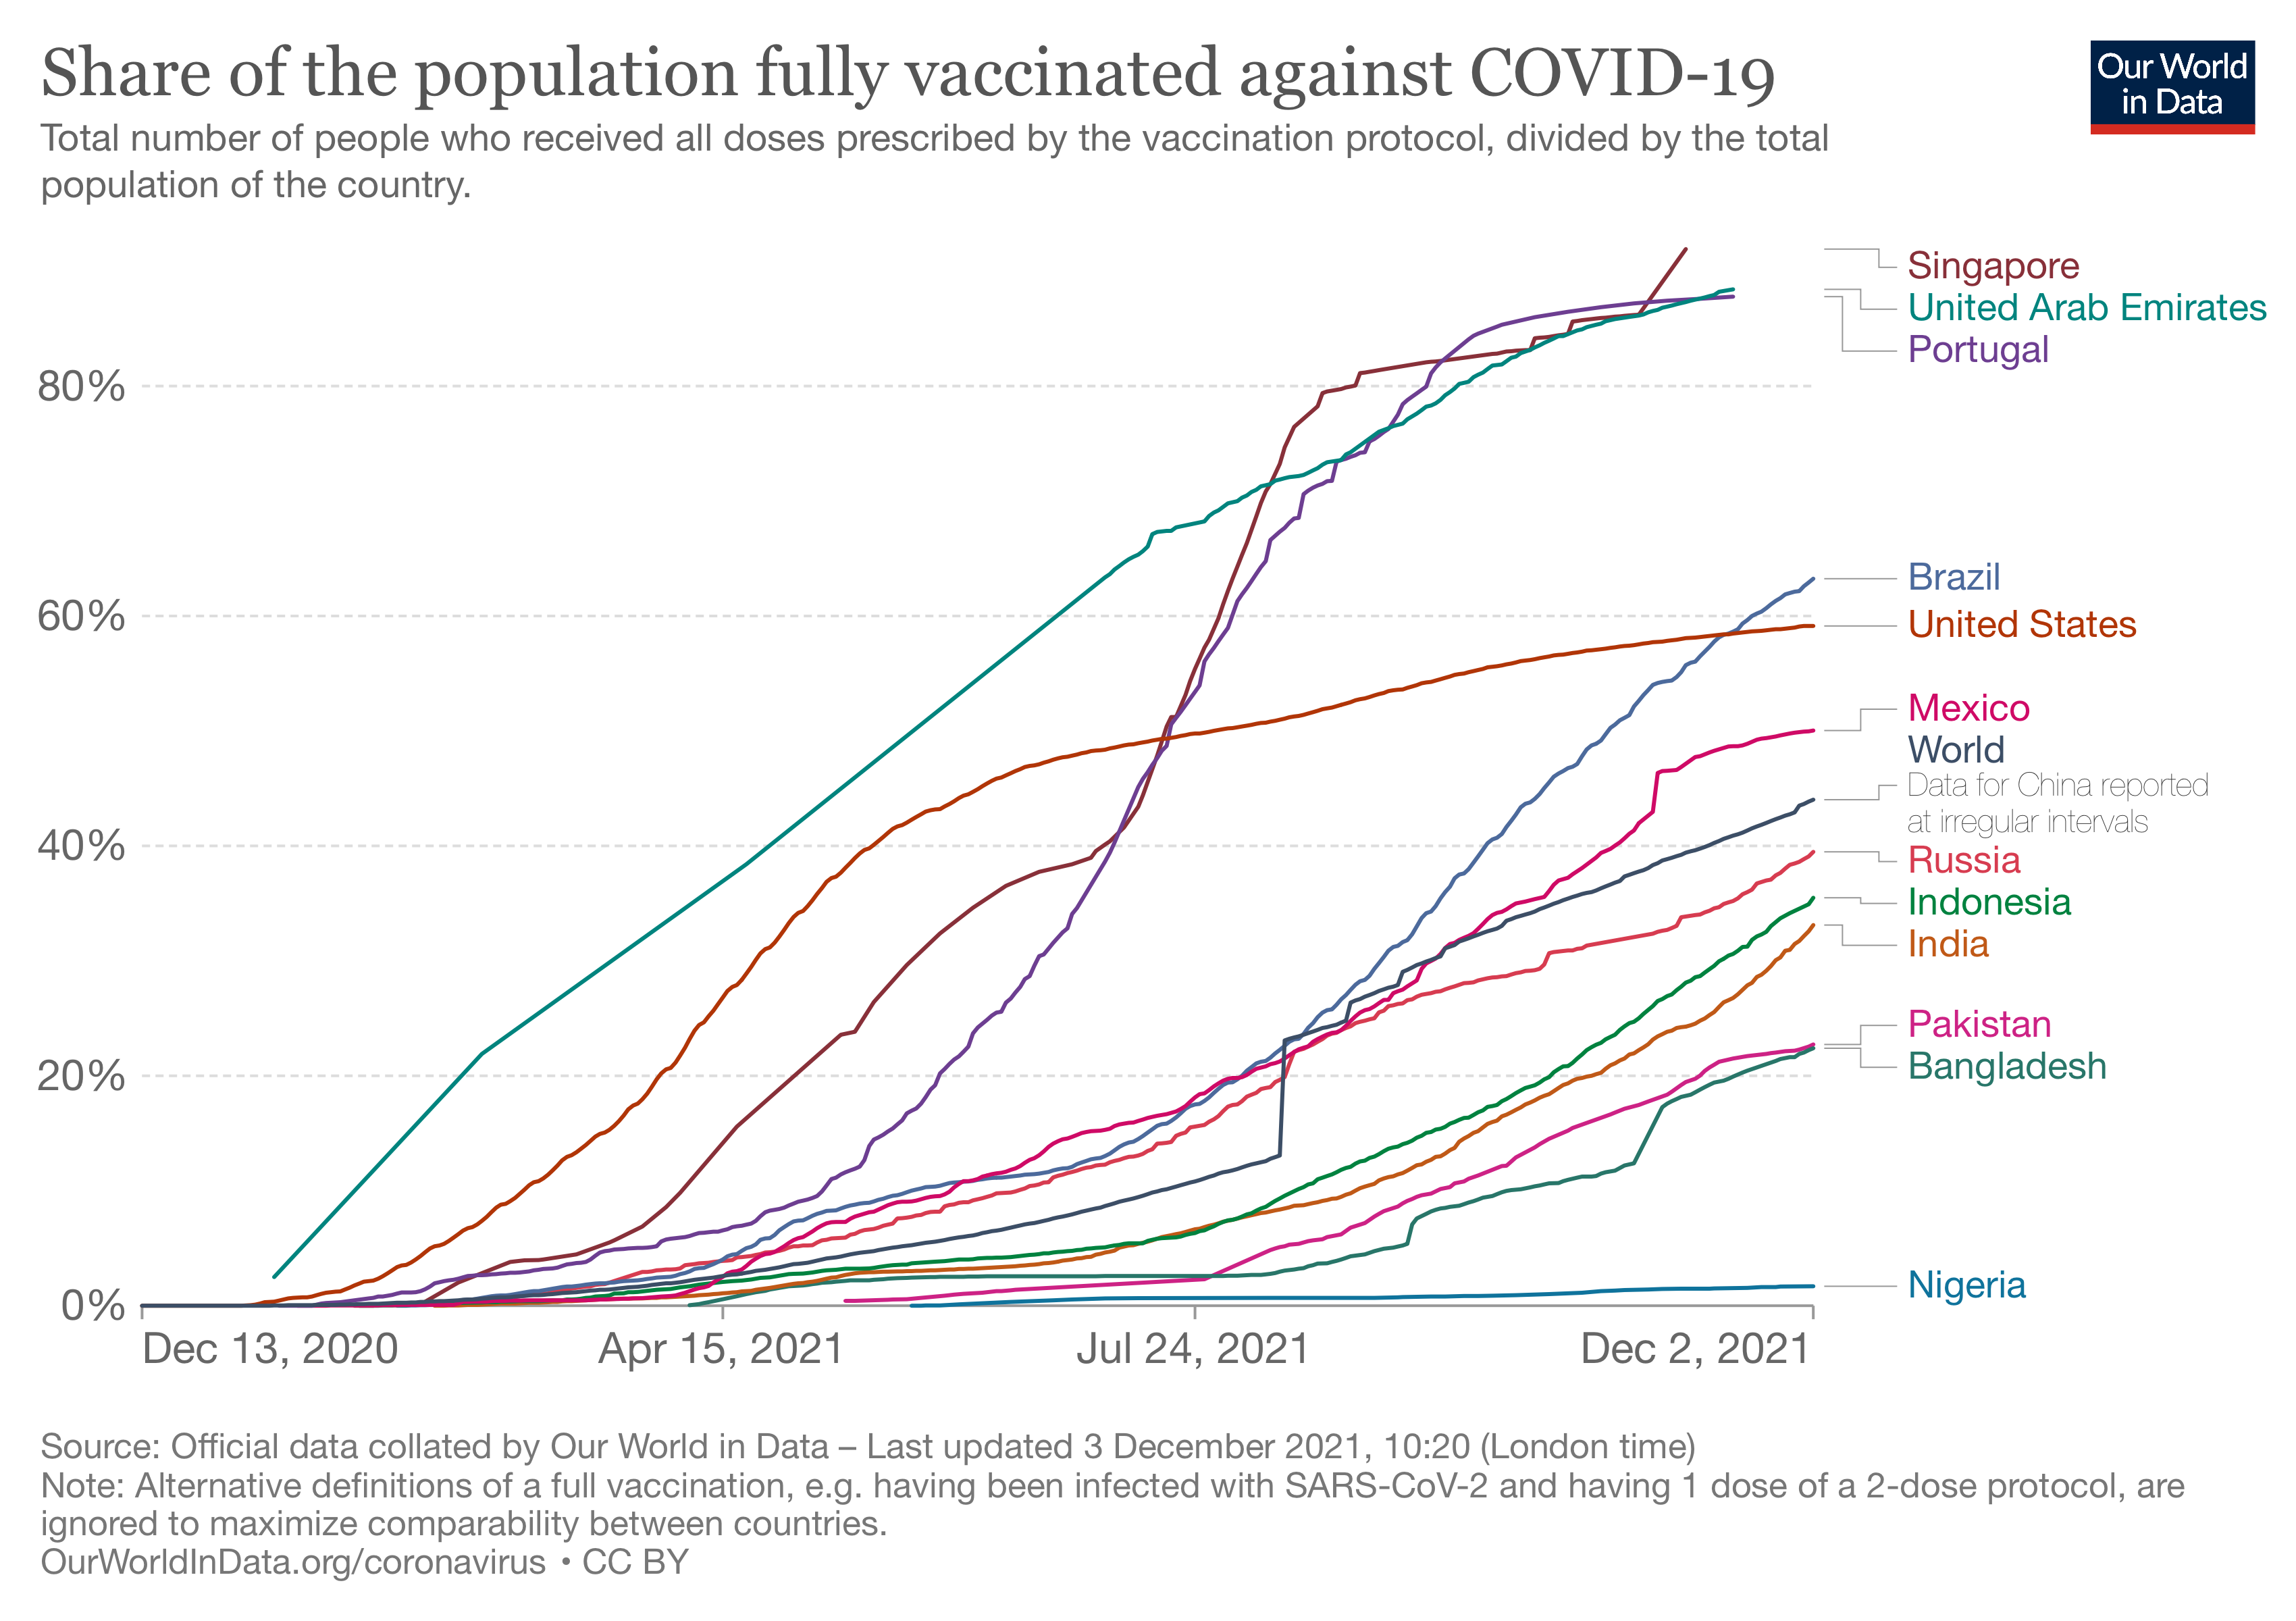
\includegraphics{./image/share-people-fully-vaccinated-covid_world.png}

As the high vaccination rate is a big part of ending pandemic by
achieving herd-immunity, our group was interested in predicting how much
high vaccination rate that countries will achieve in future. As we
expect the cumulative vaccination rate graph will follow logit function,
we set our model as a logit function. We picked 5 countries,which are
Finland, Portugal, Japan, Germany,and Hongkong for our data. The
cumulative vaccination graphs in these countries roughly follow the
logit function and our main modeling idea is to see find which model the
data fits well (seperate model or hierarchical model) and to predict the
future vaccination rate.

Down below shows the barplot of population rate who received at least
one dose of covid19 vaccine by countries in our interest.

\begin{Shaded}
\begin{Highlighting}[]
\NormalTok{knitr}\SpecialCharTok{::}\FunctionTok{include\_graphics}\NormalTok{(}\StringTok{"./image/share{-}people{-}vaccinated{-}covid.png"}\NormalTok{)}
\end{Highlighting}
\end{Shaded}

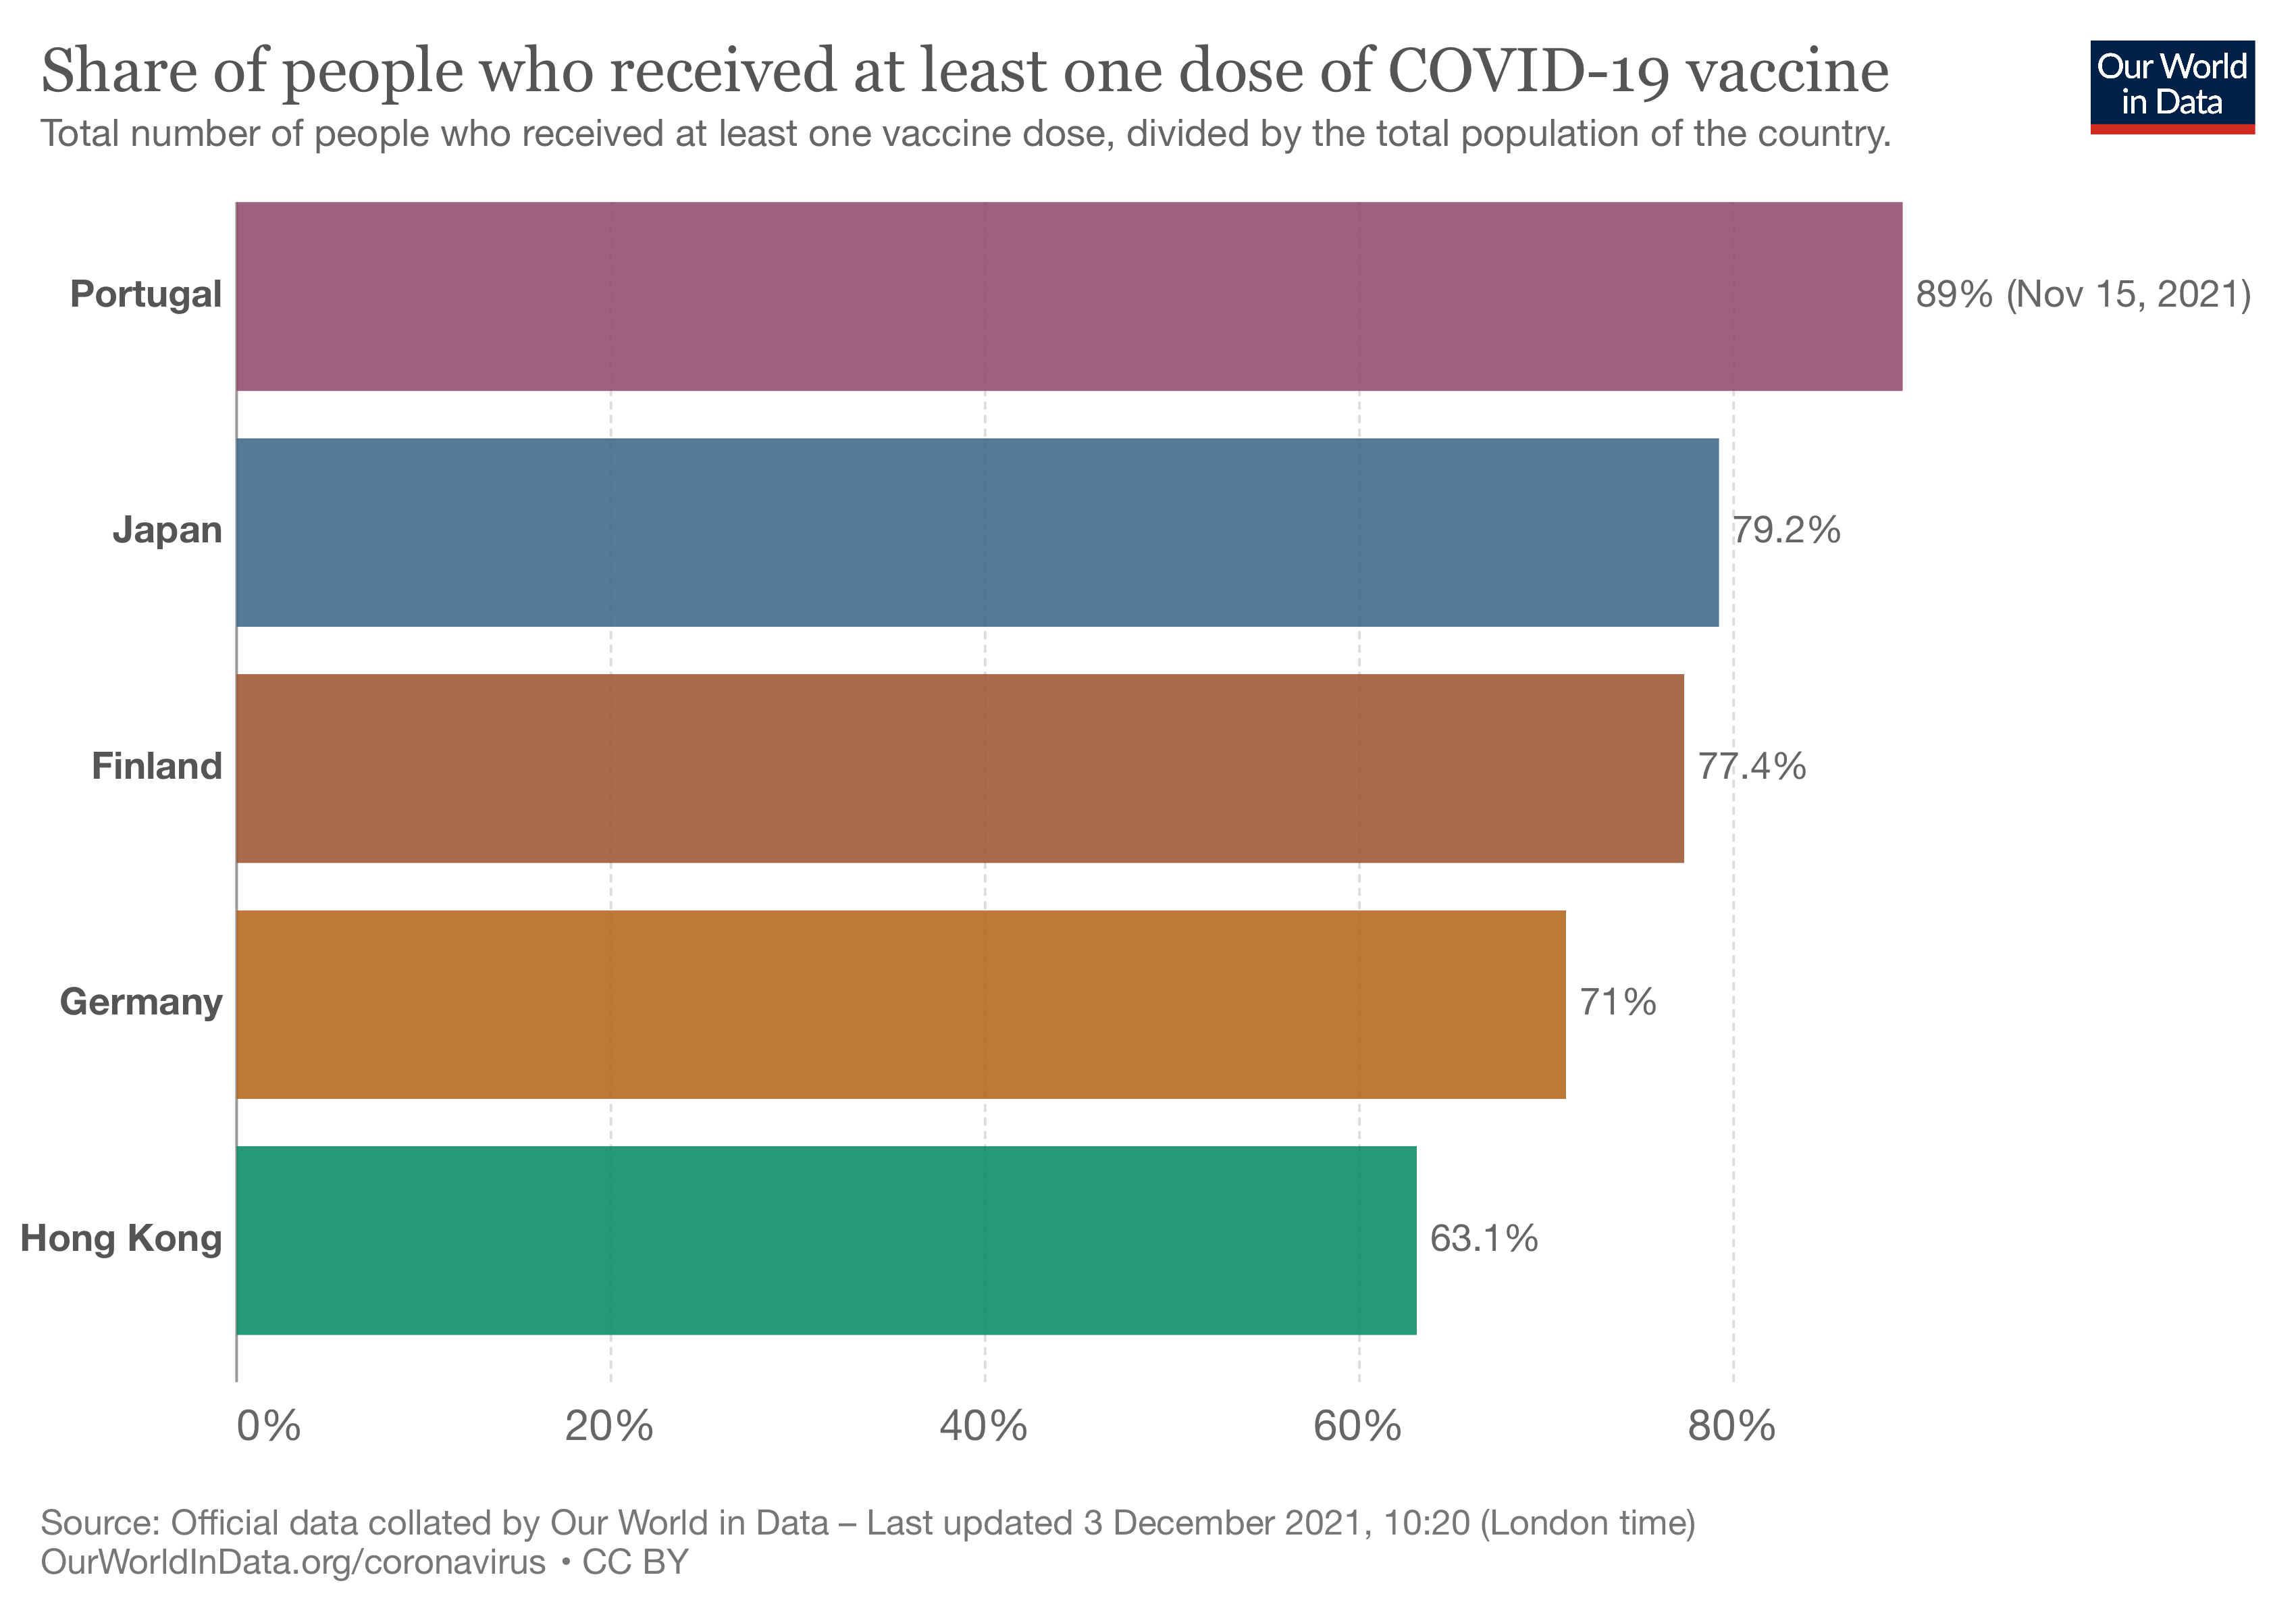
\includegraphics{./image/share-people-vaccinated-covid.png}

Down below shows the barplot of population rate of fully vaccinated
against covid19 by countries in our interest.

\begin{Shaded}
\begin{Highlighting}[]
\NormalTok{knitr}\SpecialCharTok{::}\FunctionTok{include\_graphics}\NormalTok{(}\StringTok{"./image/share{-}people{-}fully{-}vaccinated{-}covid\_bar.png"}\NormalTok{)}
\end{Highlighting}
\end{Shaded}

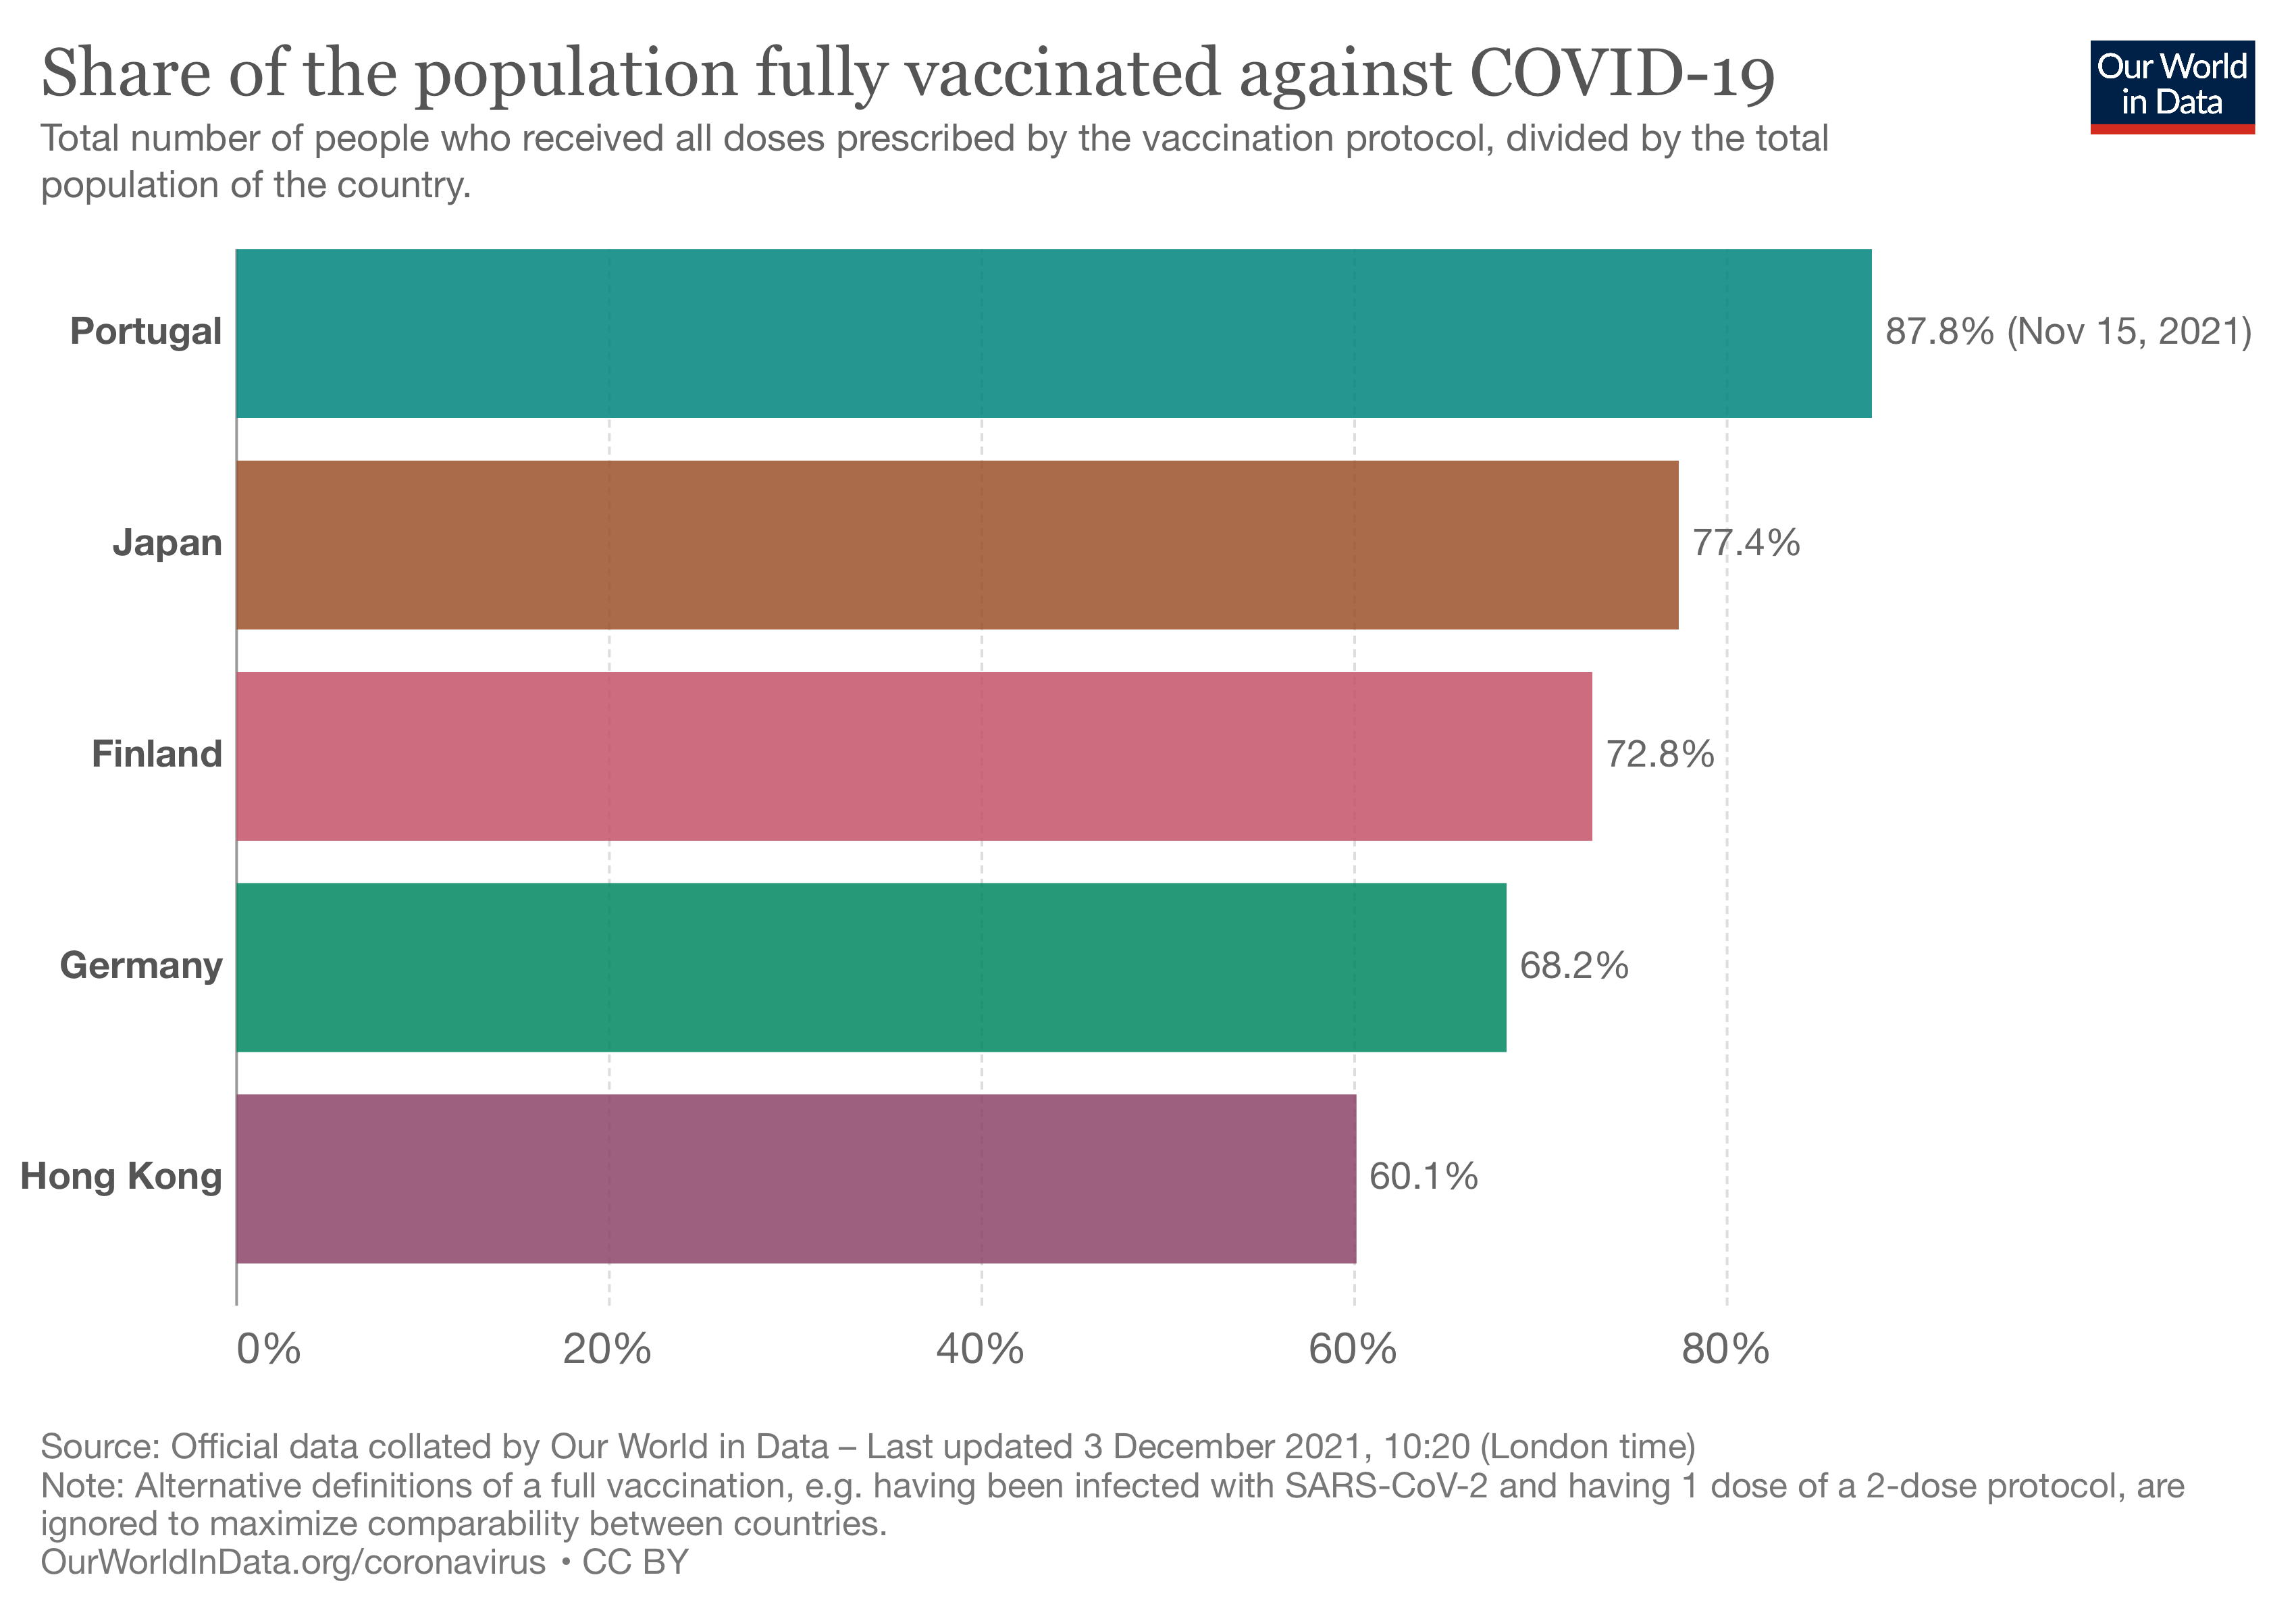
\includegraphics{./image/share-people-fully-vaccinated-covid_bar.png}

Down below shows the barplot of fully vaccinated population rate by
countries in our interest.

\begin{Shaded}
\begin{Highlighting}[]
\NormalTok{knitr}\SpecialCharTok{::}\FunctionTok{include\_graphics}\NormalTok{(}\StringTok{"./image/share{-}people{-}fully{-}vaccinated{-}covid\_plot.png"}\NormalTok{)}
\end{Highlighting}
\end{Shaded}

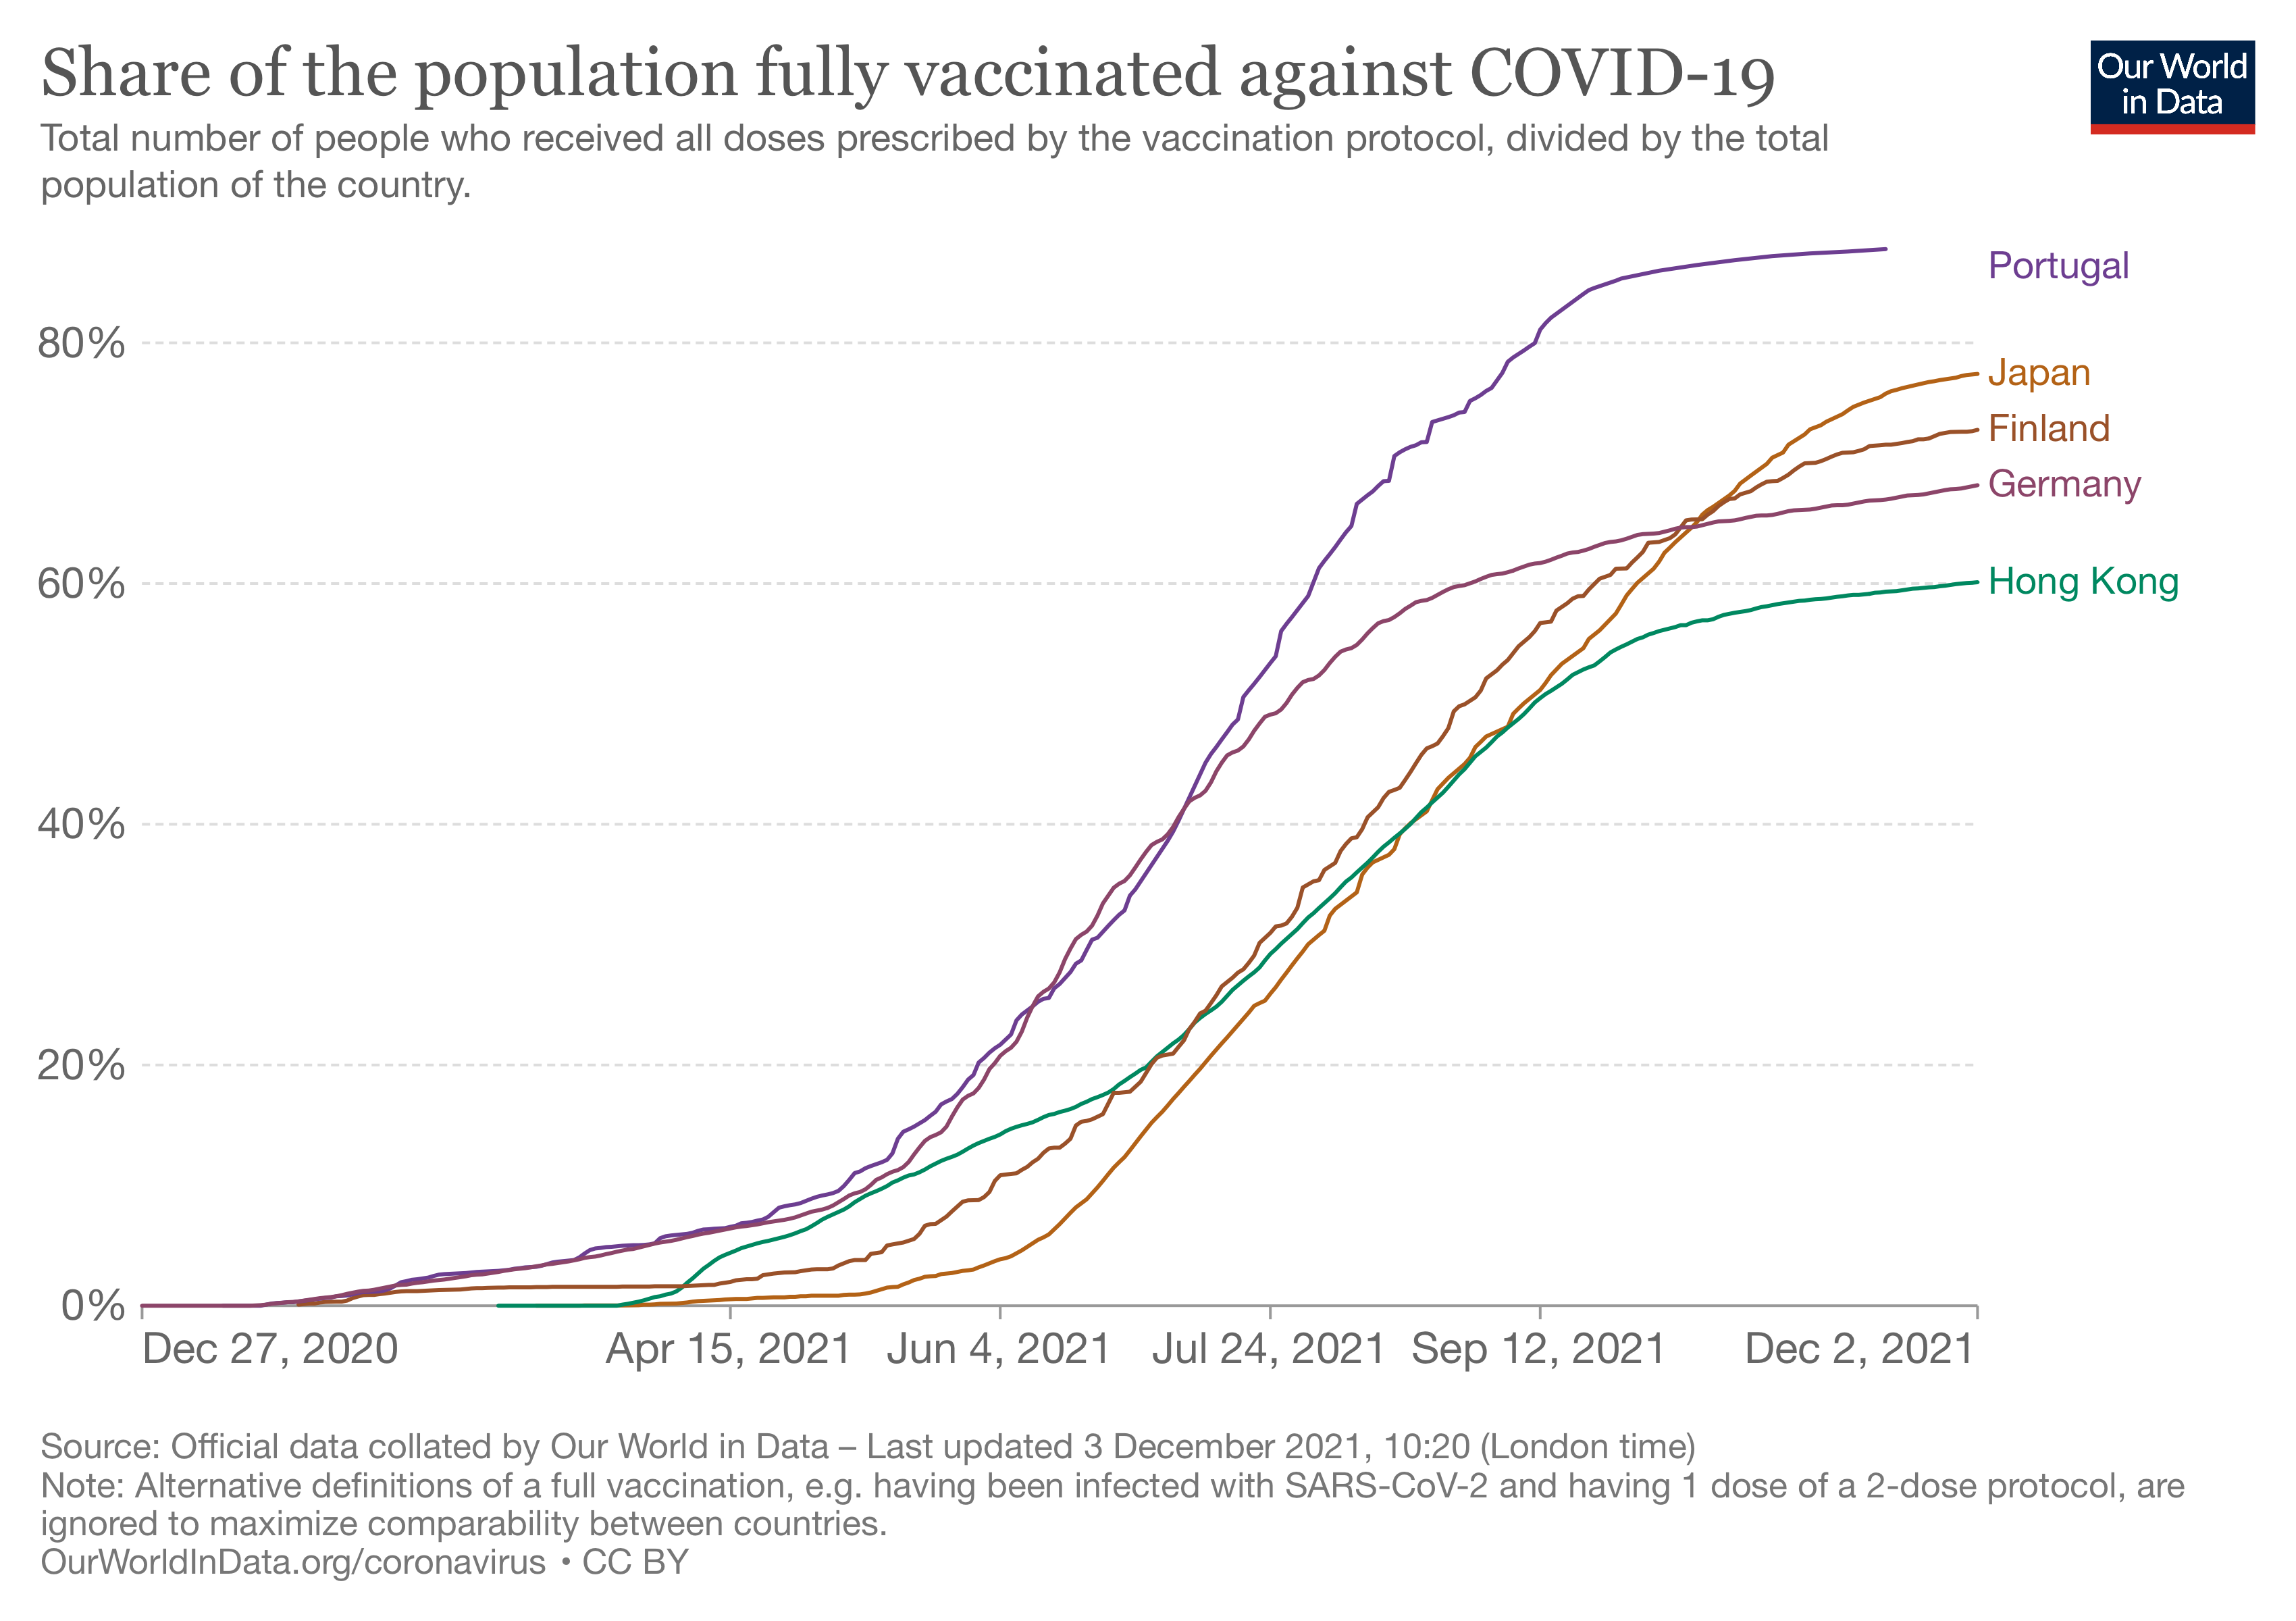
\includegraphics{./image/share-people-fully-vaccinated-covid_plot.png}

\newpage

\hypertarget{dataset}{%
\section{2. Dataset}\label{dataset}}

Datasets down below show cumulative covid vaccinations rate by
countries( collected from
\href{https://ourworldindata.org/covid-vaccinations}{linked
phrase}).Country column shows the country of this data. X column is
originally from the date when the country started vaccination to the
recent date of vaccination. We normalized the date column by giving
index 0 to number of date and deviding it with the number of date. As
the time length of the vaccination differs by country, we uniformly
picked the 222 datapoints from the datasets before normalize the X
column. Y column shows the covid vaccination rate in the country. With
the cumulative covid vaccination number, we devide it by 2 times
population because most of the vaccines require 2 doses to be fully
vaccinated. Therefore, dimension of all datasets are (222,3).

\begin{Shaded}
\begin{Highlighting}[]
\NormalTok{finland }\OtherTok{\textless{}{-}} \FunctionTok{read.csv}\NormalTok{(}\StringTok{"data/Finland\_output.csv"}\NormalTok{)}
\NormalTok{germany }\OtherTok{\textless{}{-}} \FunctionTok{read.csv}\NormalTok{(}\StringTok{"data/Germany\_output.csv"}\NormalTok{)}
\NormalTok{hongkong }\OtherTok{\textless{}{-}} \FunctionTok{read.csv}\NormalTok{(}\StringTok{\textquotesingle{}data/Hong Kong\_output.csv\textquotesingle{}}\NormalTok{)}
\NormalTok{portugal }\OtherTok{\textless{}{-}} \FunctionTok{read.csv}\NormalTok{(}\StringTok{\textquotesingle{}data/Portugal\_output.csv\textquotesingle{}}\NormalTok{)}
\NormalTok{japan }\OtherTok{\textless{}{-}} \FunctionTok{read.csv}\NormalTok{(}\StringTok{\textquotesingle{}data/Japan\_output.csv\textquotesingle{}}\NormalTok{)}
\end{Highlighting}
\end{Shaded}

\begin{Shaded}
\begin{Highlighting}[]
\FunctionTok{cat}\NormalTok{(}\StringTok{\textquotesingle{}dimenstion of Finland dataset: \textquotesingle{}}\NormalTok{,}\FunctionTok{dim}\NormalTok{(finland),}\StringTok{\textquotesingle{}}\SpecialCharTok{\textbackslash{}n}\StringTok{\textquotesingle{}}\NormalTok{)}
\end{Highlighting}
\end{Shaded}

\begin{verbatim}
## dimenstion of Finland dataset:  222 3
\end{verbatim}

\begin{Shaded}
\begin{Highlighting}[]
\FunctionTok{cat}\NormalTok{(}\StringTok{\textquotesingle{}dimenstion of Germany dataset: \textquotesingle{}}\NormalTok{,}\FunctionTok{dim}\NormalTok{(germany),}\StringTok{\textquotesingle{}}\SpecialCharTok{\textbackslash{}n}\StringTok{\textquotesingle{}}\NormalTok{)}
\end{Highlighting}
\end{Shaded}

\begin{verbatim}
## dimenstion of Germany dataset:  222 3
\end{verbatim}

\begin{Shaded}
\begin{Highlighting}[]
\FunctionTok{cat}\NormalTok{(}\StringTok{\textquotesingle{}dimenstion of HongKong dataset: \textquotesingle{}}\NormalTok{,}\FunctionTok{dim}\NormalTok{(hongkong),}\StringTok{\textquotesingle{}}\SpecialCharTok{\textbackslash{}n}\StringTok{\textquotesingle{}}\NormalTok{)}
\end{Highlighting}
\end{Shaded}

\begin{verbatim}
## dimenstion of HongKong dataset:  222 3
\end{verbatim}

\begin{Shaded}
\begin{Highlighting}[]
\FunctionTok{cat}\NormalTok{(}\StringTok{\textquotesingle{}dimenstion of Portugal dataset: \textquotesingle{}}\NormalTok{,}\FunctionTok{dim}\NormalTok{(portugal),}\StringTok{\textquotesingle{}}\SpecialCharTok{\textbackslash{}n}\StringTok{\textquotesingle{}}\NormalTok{)}
\end{Highlighting}
\end{Shaded}

\begin{verbatim}
## dimenstion of Portugal dataset:  222 3
\end{verbatim}

\begin{Shaded}
\begin{Highlighting}[]
\FunctionTok{cat}\NormalTok{(}\StringTok{\textquotesingle{}dimenstion of Japan dataset: \textquotesingle{}}\NormalTok{,}\FunctionTok{dim}\NormalTok{(japan),}\StringTok{\textquotesingle{}}\SpecialCharTok{\textbackslash{}n}\StringTok{\textquotesingle{}}\NormalTok{)}
\end{Highlighting}
\end{Shaded}

\begin{verbatim}
## dimenstion of Japan dataset:  222 3
\end{verbatim}

\begin{Shaded}
\begin{Highlighting}[]
\NormalTok{total}\OtherTok{=} \FunctionTok{rbind}\NormalTok{(finland,germany,hongkong,portugal,japan)}
\FunctionTok{ggplot}\NormalTok{(}\AttributeTok{data =}\NormalTok{ total, }\FunctionTok{aes}\NormalTok{(}\AttributeTok{x =}\NormalTok{ X, }\AttributeTok{y =}\NormalTok{ Y, }\AttributeTok{color =}\NormalTok{ Country)) }\SpecialCharTok{+}
    \FunctionTok{geom\_line}\NormalTok{() }\SpecialCharTok{+}
    \FunctionTok{ggtitle}\NormalTok{(}\StringTok{"Cumulative covid19 vaccination rate"}\NormalTok{) }\SpecialCharTok{+}
    \FunctionTok{xlab}\NormalTok{(}\StringTok{"time"}\NormalTok{) }\SpecialCharTok{+} \FunctionTok{ylab}\NormalTok{(}\StringTok{"vaccination rate"}\NormalTok{)}
\end{Highlighting}
\end{Shaded}

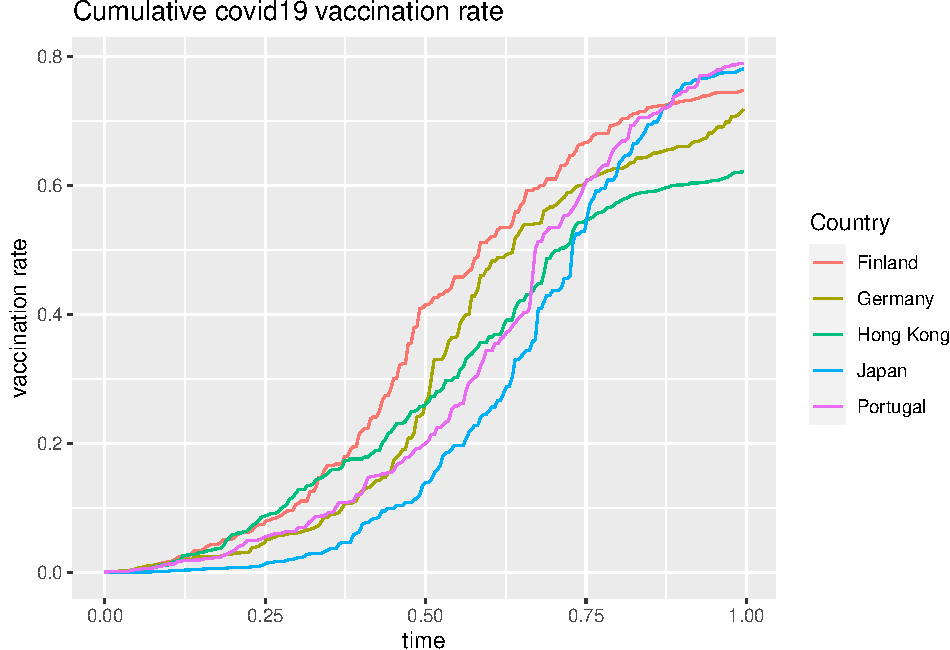
\includegraphics{bda_project_files/figure-latex/unnamed-chunk-7-1.pdf}

\newpage

\hypertarget{mathematical-models-and-stan-code}{%
\section{3. Mathematical Models and Stan
code}\label{mathematical-models-and-stan-code}}

\hypertarget{seperated-model}{%
\subsection{Seperated Model}\label{seperated-model}}

\[
\begin{aligned}
y_{i j} \mid \mu_i, \sigma &\sim \operatorname{Normal}\left(\mu_i, \sigma\right) \\
\mu_i &\sim \operatorname{logit}(\alpha_i, \beta_i)\\
\sigma &\sim \text{inv}\chi^2(1)\\
\\
\alpha_i &\sim \text{inv}\chi^2(1) \\
\beta_i &\sim N(0.5,1) \\
\end{aligned}
\]

We will first try to build the seperated model in stan

\begin{Shaded}
\begin{Highlighting}[]
\NormalTok{seperated\_model }\OtherTok{\textless{}{-}} \StringTok{"}
\StringTok{functions \{}
\StringTok{  real[] logit\_transform(real[] x, real k, real x0) \{}
\StringTok{    int N = size(x);}
\StringTok{    real xtemp[N];}
\StringTok{    for (i in 1:N)\{}
\StringTok{      xtemp[i] = 1 / (1 + exp({-}k * (x[i] {-} x0)));}
\StringTok{    \}}
\StringTok{     return xtemp;}
\StringTok{  \}}
\StringTok{\}}

\StringTok{data \{}
\StringTok{    int\textless{}lower=1\textgreater{} J;}
\StringTok{    int\textless{}lower=1\textgreater{} M;}
\StringTok{    int\textless{}lower=0\textgreater{} N; // number of data points}
\StringTok{    real x[M,N]; // observation year}
\StringTok{    real y[M,N]; // observation number of drowned}
\StringTok{    real xpred[J];  // prediction year}
\StringTok{\}}

\StringTok{parameters \{}
\StringTok{  real alpha[M];}
\StringTok{  real beta[M];}
\StringTok{  real\textless{}lower = 0\textgreater{} sigma;}
\StringTok{\}}

\StringTok{transformed parameters \{}
\StringTok{  real mu[M,N];}
\StringTok{  for (i in 1:M)\{}
\StringTok{    mu[i,] = logit\_transform(x[i,],alpha[i], beta[i]);}
\StringTok{  \}}
\StringTok{\}}

\StringTok{model \{}
\StringTok{  for (i in 1:M)\{}
\StringTok{    // as prior we will change it to the same values}
\StringTok{    alpha[i] \textasciitilde{} inv\_chi\_square(1);}
\StringTok{    beta[i] \textasciitilde{} normal(0.5,1);}
\StringTok{  \}}

\StringTok{  sigma \textasciitilde{} inv\_chi\_square(1);}

\StringTok{  //likelihood}
\StringTok{  for (i in 1:M)\{}
\StringTok{    y[i,] \textasciitilde{} normal(mu[i,], sigma);}
\StringTok{  \}}
\StringTok{\}}

\StringTok{generated quantities \{}
\StringTok{  vector[N] log\_lik[M];}
\StringTok{  real ypred[M,J];}
\StringTok{  for (i in 1:M)\{}
\StringTok{    ypred[i,] = normal\_rng(logit\_transform(xpred,alpha[i], beta[i]), sigma);}
\StringTok{  \}}

\StringTok{  //log{-}likelihood}
\StringTok{  for (i in 1:M) \{}
\StringTok{    for (j in 1:N) \{}
\StringTok{    log\_lik[i,j] = normal\_lpdf(y[i,j] | mu[i,j], sigma);}
\StringTok{    \}}
\StringTok{  \}}

\StringTok{\}}

\StringTok{"}
\end{Highlighting}
\end{Shaded}

\hypertarget{hirachical-model}{%
\subsection{Hirachical Model}\label{hirachical-model}}

\[
\begin{aligned}
y_{i j} \mid \mu_i, \sigma &\sim \operatorname{Normal}\left(\mu_i, \sigma\right) \\
\mu_i &\sim \operatorname{logit}(\alpha_i, \beta_i)\\
\sigma & \sim \operatorname{Inv}-\chi^{2}(1) \\
\\
\beta_{j}\mid \mu_{\beta}, \sigma_{\beta} &\sim \operatorname{Normal}(\mu_{\beta}, \sigma_{\beta})\\
\alpha_{j} \mid \sigma_{\alpha} & \sim \operatorname{Inv}-\chi^{2}\left(\sigma_{\alpha}\right) \\
\\
\mu_{\beta} & \sim \operatorname{Normal}(0,1)\\
\sigma_{\beta} & \sim \operatorname{Inv}-\chi^{2}(1) \\
\sigma_{\alpha} & \sim \operatorname{Inv}-\chi^{2}(1) \\
\end{aligned}
\]

Now we will build the hierarchical model in stan:

\begin{Shaded}
\begin{Highlighting}[]
\NormalTok{hierarchical\_model }\OtherTok{\textless{}{-}} \StringTok{"}
\StringTok{functions \{}
\StringTok{  real[] logit\_transform(real[] x, real k, real x0) \{}
\StringTok{    int N = size(x);}
\StringTok{    real xtemp[N];}
\StringTok{    for (i in 1:N)\{}
\StringTok{      xtemp[i] = 1 / (1 + exp({-}k * (x[i] {-} x0)));}
\StringTok{    \}}
\StringTok{     return xtemp;}
\StringTok{  \}}
\StringTok{\}}

\StringTok{data \{}
\StringTok{    int\textless{}lower = 1\textgreater{} J; //number of predictions}
\StringTok{    int\textless{}lower=1\textgreater{} M; //number of country}
\StringTok{    int\textless{}lower=0\textgreater{} N; // number of data points}
\StringTok{    real x[M,N]; //}
\StringTok{    real y[M,N]; //}
\StringTok{    real xpred[J];  // prediction year}
\StringTok{\}}

\StringTok{parameters \{}
\StringTok{  real alpha[M];}
\StringTok{  real beta[M];}
\StringTok{  real\textless{}lower = 0\textgreater{} sigma;}
\StringTok{  real\textless{}lower = 0\textgreater{} hyper\_sigma;}
\StringTok{  real hyper\_mu;}
\StringTok{  real\textless{}lower = 0\textgreater{} hyper\_alpha;}
\StringTok{\}}

\StringTok{transformed parameters \{}
\StringTok{  real mu[M,N];}
\StringTok{  for (i in 1:M)\{}
\StringTok{    mu[i,] = logit\_transform(x[i,],alpha[i], beta[i]);}
\StringTok{  \}}
\StringTok{\}}

\StringTok{model \{}
\StringTok{    hyper\_mu \textasciitilde{} normal(0, 1);}
\StringTok{    hyper\_sigma \textasciitilde{} inv\_chi\_square(10);}
\StringTok{    hyper\_alpha \textasciitilde{} inv\_chi\_square(10);}

\StringTok{  for (i in 1:M)\{}
\StringTok{    // as prior we will change it to the same values}
\StringTok{    alpha[i] \textasciitilde{} inv\_chi\_square(hyper\_alpha);}
\StringTok{    beta[i] \textasciitilde{} normal(hyper\_mu,hyper\_sigma);}
\StringTok{  \}}

\StringTok{  sigma \textasciitilde{} inv\_chi\_square(1);}

\StringTok{  //likelihood}
\StringTok{  for (i in 1:M)\{}
\StringTok{    y[i,] \textasciitilde{} normal(mu[i,], sigma);}
\StringTok{  \}}
\StringTok{\}}

\StringTok{generated quantities \{}
\StringTok{  vector[N] log\_lik[M];}
\StringTok{  real ypred[M,J];}
\StringTok{  for (i in 1:M)\{}
\StringTok{    ypred[i,] = normal\_rng(logit\_transform(xpred,alpha[i], beta[i]), sigma);}
\StringTok{  \}}

\StringTok{  //log{-}likelihood}
\StringTok{  for (i in 1:M) \{}
\StringTok{    for (j in 1:N) \{}
\StringTok{    log\_lik[i,j] = normal\_lpdf(y[i,j] | mu[i,j], sigma);}
\StringTok{    \}}
\StringTok{  \}}

\StringTok{\}}

\StringTok{"}
\end{Highlighting}
\end{Shaded}

\newpage

\hypertarget{prior-selection}{%
\section{4. Prior selection}\label{prior-selection}}

For both models we choose to use weakly informative priors. We will
first present all prior distribuions in plots, to visualize better their
properties.

\begin{Shaded}
\begin{Highlighting}[]
\NormalTok{x }\OtherTok{\textless{}{-}} \FunctionTok{seq}\NormalTok{(}\AttributeTok{from=}\FloatTok{0.1}\NormalTok{, }\AttributeTok{to=}\DecValTok{5}\NormalTok{, }\AttributeTok{by=}\FloatTok{0.01}\NormalTok{)}
\FunctionTok{plot}\NormalTok{(x, }\FunctionTok{dinvchisq}\NormalTok{(x,}\DecValTok{1}\NormalTok{,}\DecValTok{1}\NormalTok{), }\AttributeTok{ylim=}\FunctionTok{c}\NormalTok{(}\DecValTok{0}\NormalTok{,}\DecValTok{1}\NormalTok{), }\AttributeTok{type=}\StringTok{"l"}\NormalTok{, }\AttributeTok{main=}\StringTok{"inv{-}chi{-}square(1) PDF"}\NormalTok{,}
     \AttributeTok{ylab=}\StringTok{"density"}\NormalTok{, }\AttributeTok{col=}\StringTok{"red"}\NormalTok{)}
\end{Highlighting}
\end{Shaded}

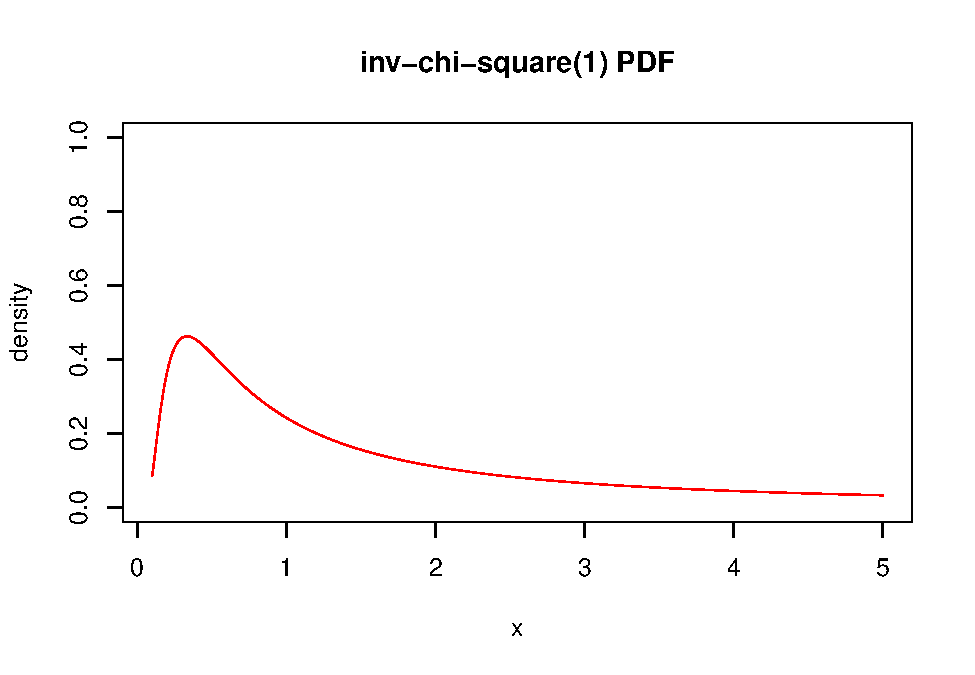
\includegraphics{bda_project_files/figure-latex/unnamed-chunk-10-1.pdf}

\begin{Shaded}
\begin{Highlighting}[]
\NormalTok{x }\OtherTok{\textless{}{-}} \FunctionTok{seq}\NormalTok{(}\AttributeTok{from=}\SpecialCharTok{{-}}\DecValTok{5}\NormalTok{, }\AttributeTok{to=}\DecValTok{5}\NormalTok{, }\AttributeTok{by=}\FloatTok{0.01}\NormalTok{)}
\FunctionTok{plot}\NormalTok{(x, }\FunctionTok{dnorm}\NormalTok{(x, }\FloatTok{0.5}\NormalTok{, }\DecValTok{1}\NormalTok{), }\AttributeTok{ylim=}\FunctionTok{c}\NormalTok{(}\DecValTok{0}\NormalTok{,}\DecValTok{1}\NormalTok{), }\AttributeTok{type=}\StringTok{"l"}\NormalTok{, }\AttributeTok{main=}\StringTok{"Normal(0.5,1) PDF"}\NormalTok{,}
     \AttributeTok{ylab=}\StringTok{"density"}\NormalTok{, }\AttributeTok{col=}\StringTok{"red"}\NormalTok{)}
\end{Highlighting}
\end{Shaded}

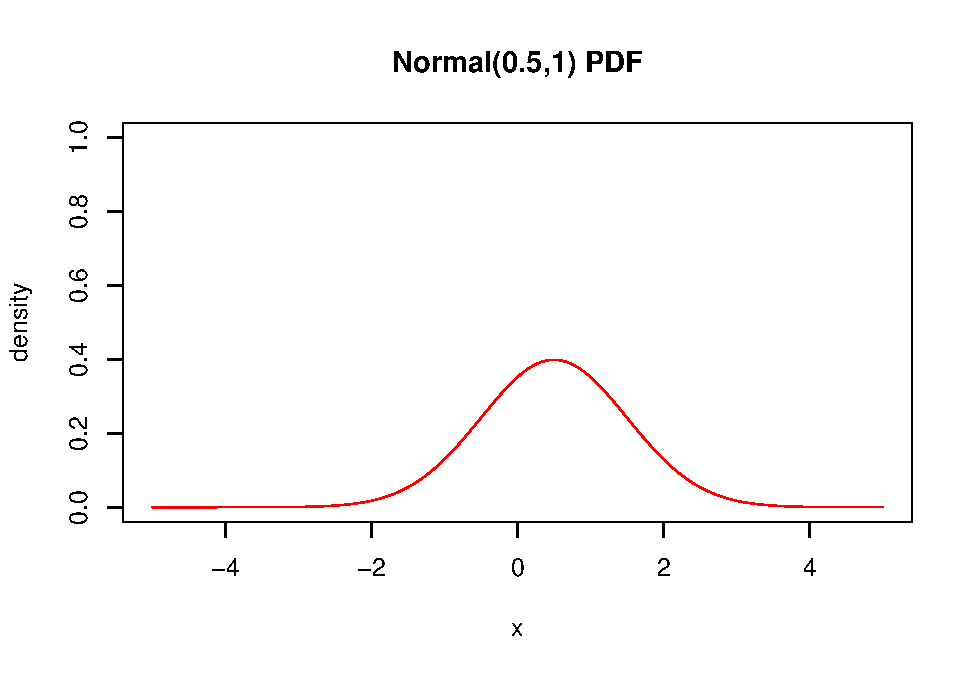
\includegraphics{bda_project_files/figure-latex/unnamed-chunk-11-1.pdf}

\begin{Shaded}
\begin{Highlighting}[]
\NormalTok{x }\OtherTok{\textless{}{-}} \FunctionTok{seq}\NormalTok{(}\AttributeTok{from=}\SpecialCharTok{{-}}\DecValTok{5}\NormalTok{, }\AttributeTok{to=}\DecValTok{5}\NormalTok{, }\AttributeTok{by=}\FloatTok{0.01}\NormalTok{)}
\FunctionTok{plot}\NormalTok{(x, }\FunctionTok{dnorm}\NormalTok{(x, }\DecValTok{0}\NormalTok{, }\DecValTok{1}\NormalTok{), }\AttributeTok{ylim=}\FunctionTok{c}\NormalTok{(}\DecValTok{0}\NormalTok{,}\DecValTok{1}\NormalTok{), }\AttributeTok{type=}\StringTok{"l"}\NormalTok{, }\AttributeTok{main=}\StringTok{"Normal(0,1) PDF"}\NormalTok{,}
     \AttributeTok{ylab=}\StringTok{"density"}\NormalTok{, }\AttributeTok{col=}\StringTok{"red"}\NormalTok{)}
\end{Highlighting}
\end{Shaded}

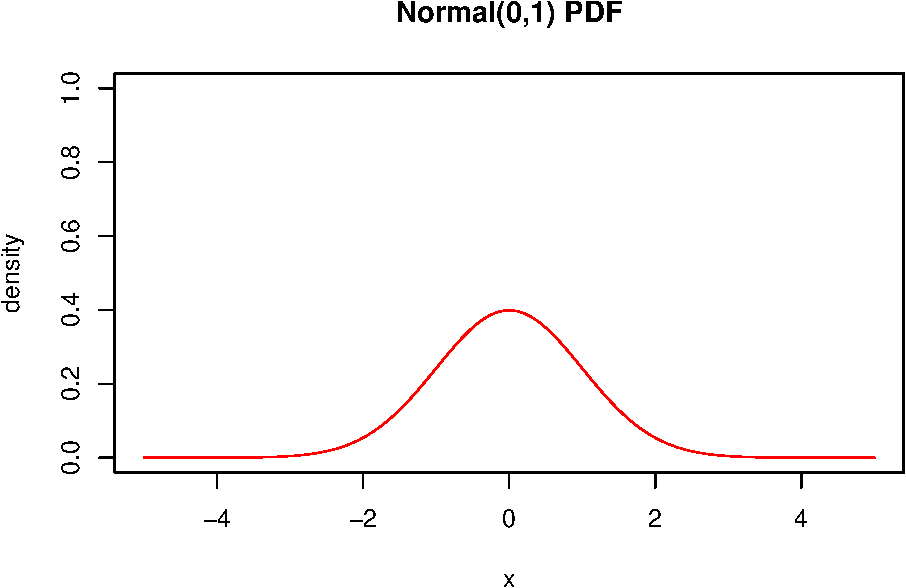
\includegraphics{bda_project_files/figure-latex/unnamed-chunk-12-1.pdf}

\hypertarget{prior-choice-of-the-seperated-model}{%
\subsection{Prior choice of the seperated
model}\label{prior-choice-of-the-seperated-model}}

For the seperated model, the \(\alpha\) prior needed to fullfill two
criteria. First it needed to be a positive number, as we can expect from
the vaccination, that the rate is rising and not dropping. Also, as the
vaccination should follow roughly a logit function, as it can be
observed from the data, we can expect to have a gradient, which is more
likely around \(1\) than bigger than \(50\). Hence the prior of
\(\operatorname{Inv}-\chi^{2}(1)\) was choosen.

For our \(\beta\) prior estimation we know, that it should be in the
range of \([0,1]\), as this is the range of our x-Data. Therefore we
choose \(N(0.5,1)\).

The variance of our y-sampling should be a positive number. As we can
also expect it to be quite small, as we want our model following the
line quite tightly, we choose here as well
\(\operatorname{Inv}-\chi^{2}(1)\).

\hypertarget{prior-choices-of-the-hirachical-model}{%
\subsection{Prior choices of the hirachical
model}\label{prior-choices-of-the-hirachical-model}}

The hirachical model has the following priors. The \(\alpha\)- prior
still has the same distribution function:
\(\operatorname{Inv}-\chi^{2}(\cdot)\), with the same reasoning as for
the seperated model. Here however, the parameter for the function gets
sampled as well. With the same reasoning about the order of magnitude of
our parameter we choose \(\operatorname{Inv}-\chi^{2}(1)\) as a suitable
weakly informative prior. As we can see in the plot above, the PDF of
the probability distribution has nearly all amount of its mass in the
interval of \([0,10]\)

The \(\beta\) prior is again, like in the seperated model a normal
distribution \(N(\cdot,\cdot)\). For the first argument, we choose a
normal distribution of \(N(0,1)\), with the reasoning, that we expect it
to be located somewhere in the interval of \([0,1]\), as this is the
range of the data. The prior of the variance is given by a
\(\operatorname{Inv}-\chi^{2}(1)\), as here as well we want to have a
variance, which is not much larger, than our expected interval.

\newpage

\hypertarget{stan-code}{%
\section{5. Stan code}\label{stan-code}}

The stan code was provided above with the describtion of the model

\newpage

\hypertarget{how-to-the-stan-model-was-run-that-is-what-options-were-used.-this-is-also-more-clear-as-combination-of-textual-explanation-and-the-actual-code-line}{%
\section{6. How to the Stan model was run, that is, what options were
used. This is also more clear as combination of textual explanation and
the actual code
line}\label{how-to-the-stan-model-was-run-that-is-what-options-were-used.-this-is-also-more-clear-as-combination-of-textual-explanation-and-the-actual-code-line}}

\begin{Shaded}
\begin{Highlighting}[]
\CommentTok{\# setwd("/Users/max/Documents/UniMac/Aalto/BDA/bda\_aalto\_project/data")}
\CommentTok{\#setwd("/home/chooh1/notebooks/BDA/project")}
\NormalTok{finland }\OtherTok{\textless{}{-}} \FunctionTok{read.csv}\NormalTok{(}\StringTok{"data/Finland\_output.csv"}\NormalTok{)}
\NormalTok{germany }\OtherTok{\textless{}{-}} \FunctionTok{read.csv}\NormalTok{(}\StringTok{"data/Germany\_output.csv"}\NormalTok{)}
\NormalTok{portugal }\OtherTok{\textless{}{-}} \FunctionTok{read.csv}\NormalTok{(}\StringTok{"data/Portugal\_output.csv"}\NormalTok{)}
\NormalTok{hongkong }\OtherTok{\textless{}{-}} \FunctionTok{read.csv}\NormalTok{(}\StringTok{"data/Hong Kong\_output.csv"}\NormalTok{)}
\NormalTok{japan }\OtherTok{\textless{}{-}} \FunctionTok{read.csv}\NormalTok{(}\StringTok{"data/Japan\_output.csv"}\NormalTok{)}
\end{Highlighting}
\end{Shaded}

\begin{Shaded}
\begin{Highlighting}[]
\CommentTok{\#seperate model run}
\NormalTok{xData }\OtherTok{\textless{}{-}} \FunctionTok{rbind}\NormalTok{(finland}\SpecialCharTok{$}\NormalTok{X,germany}\SpecialCharTok{$}\NormalTok{X,portugal}\SpecialCharTok{$}\NormalTok{X,hongkong}\SpecialCharTok{$}\NormalTok{X,japan}\SpecialCharTok{$}\NormalTok{X) }\CommentTok{\#(5,222)}
\NormalTok{yData }\OtherTok{\textless{}{-}}\FunctionTok{rbind}\NormalTok{(finland}\SpecialCharTok{$}\NormalTok{Y,germany}\SpecialCharTok{$}\NormalTok{Y,portugal}\SpecialCharTok{$}\NormalTok{Y,hongkong}\SpecialCharTok{$}\NormalTok{Y,japan}\SpecialCharTok{$}\NormalTok{Y) }\CommentTok{\#(5,222)}
\NormalTok{xpred }\OtherTok{\textless{}{-}} \FunctionTok{c}\NormalTok{(}\FloatTok{1.1}\NormalTok{)}
\FunctionTok{dim}\NormalTok{(xpred) }\OtherTok{\textless{}{-}} \FunctionTok{c}\NormalTok{(}\DecValTok{1}\NormalTok{)}
\NormalTok{sm }\OtherTok{\textless{}{-}}\NormalTok{ rstan}\SpecialCharTok{::}\FunctionTok{stan\_model}\NormalTok{(}\AttributeTok{model\_code =}\NormalTok{ seperated\_model)}
\NormalTok{stan\_data }\OtherTok{\textless{}{-}} \FunctionTok{list}\NormalTok{(}
    \AttributeTok{J =} \FunctionTok{dim}\NormalTok{(xData)[}\DecValTok{2}\NormalTok{]}\SpecialCharTok{+}\DecValTok{1}\NormalTok{,}
    \AttributeTok{N =} \FunctionTok{dim}\NormalTok{(xData)[}\DecValTok{2}\NormalTok{],}
    \AttributeTok{M =} \FunctionTok{dim}\NormalTok{(xData)[}\DecValTok{1}\NormalTok{],}
    \AttributeTok{y =}\NormalTok{ yData,}
    \AttributeTok{x =}\NormalTok{ xData,}
    \AttributeTok{xpred =} \FunctionTok{c}\NormalTok{(finland}\SpecialCharTok{$}\NormalTok{X,}\FloatTok{1.1}\NormalTok{)}
\NormalTok{)}
\NormalTok{model\_separated }\OtherTok{\textless{}{-}}\NormalTok{ rstan}\SpecialCharTok{::}\FunctionTok{sampling}\NormalTok{(sm, }\AttributeTok{data =}\NormalTok{ stan\_data, }\AttributeTok{warmup=}\DecValTok{3000}\NormalTok{,}\AttributeTok{iter=}\DecValTok{4000}\NormalTok{)}
\NormalTok{fit\_sm }\OtherTok{\textless{}{-}} \FunctionTok{extract}\NormalTok{(model\_separated, }\AttributeTok{permuted =} \ConstantTok{TRUE}\NormalTok{, }\AttributeTok{inc\_warmup =} \ConstantTok{FALSE}\NormalTok{)}
\end{Highlighting}
\end{Shaded}

Below graph shows the posterior vaccination rate by countries in
seperate model.

\begin{Shaded}
\begin{Highlighting}[]
\NormalTok{Y\_s }\OtherTok{=} \FunctionTok{c}\NormalTok{(fit\_sm}\SpecialCharTok{$}\NormalTok{mu[}\DecValTok{3000}\NormalTok{,}\DecValTok{1}\NormalTok{,}\DecValTok{1}\SpecialCharTok{:}\DecValTok{222}\NormalTok{],fit\_sm}\SpecialCharTok{$}\NormalTok{mu[}\DecValTok{3000}\NormalTok{,}\DecValTok{2}\NormalTok{,}\DecValTok{1}\SpecialCharTok{:}\DecValTok{222}\NormalTok{],fit\_sm}\SpecialCharTok{$}\NormalTok{mu[}\DecValTok{3000}\NormalTok{,}\DecValTok{3}\NormalTok{,}\DecValTok{1}\SpecialCharTok{:}\DecValTok{222}\NormalTok{],}
\NormalTok{      fit\_sm}\SpecialCharTok{$}\NormalTok{mu[}\DecValTok{3000}\NormalTok{,}\DecValTok{4}\NormalTok{,}\DecValTok{1}\SpecialCharTok{:}\DecValTok{222}\NormalTok{],fit\_sm}\SpecialCharTok{$}\NormalTok{mu[}\DecValTok{3000}\NormalTok{,}\DecValTok{5}\NormalTok{,}\DecValTok{1}\SpecialCharTok{:}\DecValTok{222}\NormalTok{])}
\NormalTok{result\_s }\OtherTok{=} \FunctionTok{data.frame}\NormalTok{(}\AttributeTok{Country=}\NormalTok{total}\SpecialCharTok{$}\NormalTok{Country,}\AttributeTok{X=}\NormalTok{total}\SpecialCharTok{$}\NormalTok{X,}\AttributeTok{Y=}\NormalTok{Y\_s)}
\FunctionTok{ggplot}\NormalTok{(}\AttributeTok{data =}\NormalTok{ result\_s, }\FunctionTok{aes}\NormalTok{(}\AttributeTok{x =}\NormalTok{X, }\AttributeTok{y =}\NormalTok{ Y, }\AttributeTok{color =}\NormalTok{ Country)) }\SpecialCharTok{+}
    \FunctionTok{geom\_line}\NormalTok{() }\SpecialCharTok{+}
    \FunctionTok{ggtitle}\NormalTok{(}\StringTok{"Sampled covid19 vaccination rate from the seperated model"}\NormalTok{) }\SpecialCharTok{+}
    \FunctionTok{xlab}\NormalTok{(}\StringTok{"time"}\NormalTok{) }\SpecialCharTok{+} \FunctionTok{ylab}\NormalTok{(}\StringTok{"posterior vaccination rate"}\NormalTok{)}
\end{Highlighting}
\end{Shaded}

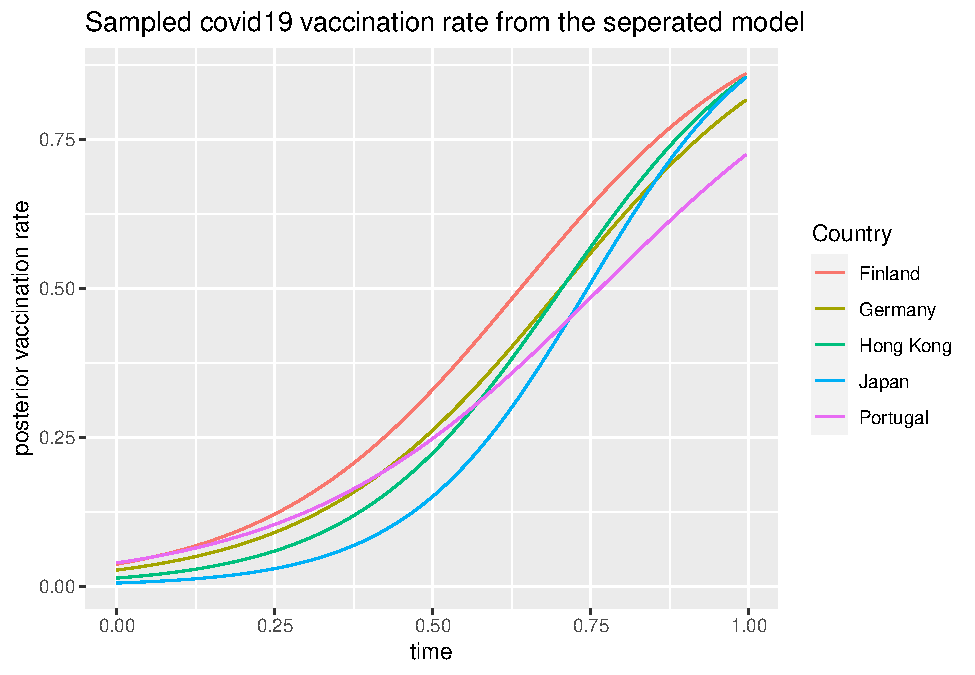
\includegraphics{bda_project_files/figure-latex/unnamed-chunk-15-1.pdf}

\begin{Shaded}
\begin{Highlighting}[]
\CommentTok{\#hierarchical model run}
\NormalTok{hm }\OtherTok{\textless{}{-}}\NormalTok{ rstan}\SpecialCharTok{::}\FunctionTok{stan\_model}\NormalTok{(}\AttributeTok{model\_code =}\NormalTok{ hierarchical\_model)}
\NormalTok{stan\_data }\OtherTok{\textless{}{-}} \FunctionTok{list}\NormalTok{(}
    \AttributeTok{J =} \FunctionTok{dim}\NormalTok{(xData)[}\DecValTok{2}\NormalTok{]}\SpecialCharTok{+}\DecValTok{1}\NormalTok{,}
    \AttributeTok{N =} \FunctionTok{dim}\NormalTok{(xData)[}\DecValTok{2}\NormalTok{],}
    \AttributeTok{M =} \FunctionTok{dim}\NormalTok{(xData)[}\DecValTok{1}\NormalTok{],}
    \AttributeTok{y =}\NormalTok{ yData,}
    \AttributeTok{x =}\NormalTok{ xData,}
    \AttributeTok{xpred =} \FunctionTok{c}\NormalTok{(finland}\SpecialCharTok{$}\NormalTok{X,}\FloatTok{1.1}\NormalTok{)}
\NormalTok{)}
\NormalTok{model\_hierarchical }\OtherTok{\textless{}{-}}\NormalTok{ rstan}\SpecialCharTok{::}\FunctionTok{sampling}\NormalTok{(hm, }\AttributeTok{data =}\NormalTok{ stan\_data, }
                                      \AttributeTok{warmup=}\DecValTok{3000}\NormalTok{,}\AttributeTok{iter=}\DecValTok{4000}\NormalTok{)}
\NormalTok{fit\_hm }\OtherTok{\textless{}{-}} \FunctionTok{extract}\NormalTok{(model\_hierarchical, }\AttributeTok{permuted =} \ConstantTok{TRUE}\NormalTok{, }\AttributeTok{inc\_warmup =} \ConstantTok{FALSE}\NormalTok{)}
\end{Highlighting}
\end{Shaded}

Below graph shows the posterior vaccination rate by countries in
hierarchical model.

\begin{Shaded}
\begin{Highlighting}[]
\NormalTok{Y\_h }\OtherTok{=} \FunctionTok{c}\NormalTok{(fit\_hm}\SpecialCharTok{$}\NormalTok{mu[}\DecValTok{3000}\NormalTok{,}\DecValTok{1}\NormalTok{,}\DecValTok{1}\SpecialCharTok{:}\DecValTok{222}\NormalTok{],fit\_hm}\SpecialCharTok{$}\NormalTok{mu[}\DecValTok{3000}\NormalTok{,}\DecValTok{2}\NormalTok{,}\DecValTok{1}\SpecialCharTok{:}\DecValTok{222}\NormalTok{],fit\_hm}\SpecialCharTok{$}\NormalTok{mu[}\DecValTok{3000}\NormalTok{,}\DecValTok{3}\NormalTok{,}\DecValTok{1}\SpecialCharTok{:}\DecValTok{222}\NormalTok{],}
\NormalTok{      fit\_hm}\SpecialCharTok{$}\NormalTok{mu[}\DecValTok{3000}\NormalTok{,}\DecValTok{4}\NormalTok{,}\DecValTok{1}\SpecialCharTok{:}\DecValTok{222}\NormalTok{],fit\_hm}\SpecialCharTok{$}\NormalTok{mu[}\DecValTok{3000}\NormalTok{,}\DecValTok{5}\NormalTok{,}\DecValTok{1}\SpecialCharTok{:}\DecValTok{222}\NormalTok{])}
\NormalTok{result\_h }\OtherTok{=} \FunctionTok{data.frame}\NormalTok{(}\AttributeTok{Country=}\NormalTok{total}\SpecialCharTok{$}\NormalTok{Country,}\AttributeTok{X=}\NormalTok{total}\SpecialCharTok{$}\NormalTok{X,}\AttributeTok{Y=}\NormalTok{Y\_h)}
\FunctionTok{ggplot}\NormalTok{(}\AttributeTok{data =}\NormalTok{ result\_h, }\FunctionTok{aes}\NormalTok{(}\AttributeTok{x =}\NormalTok{X, }\AttributeTok{y =}\NormalTok{ Y, }\AttributeTok{color =}\NormalTok{ Country)) }\SpecialCharTok{+}
    \FunctionTok{geom\_line}\NormalTok{() }\SpecialCharTok{+}
    \FunctionTok{ggtitle}\NormalTok{(}\StringTok{"Sampled covid19 vaccination rate from the hierarchical model"}\NormalTok{) }\SpecialCharTok{+}
    \FunctionTok{xlab}\NormalTok{(}\StringTok{"time"}\NormalTok{) }\SpecialCharTok{+} \FunctionTok{ylab}\NormalTok{(}\StringTok{"posterior vaccination rate"}\NormalTok{)}
\end{Highlighting}
\end{Shaded}

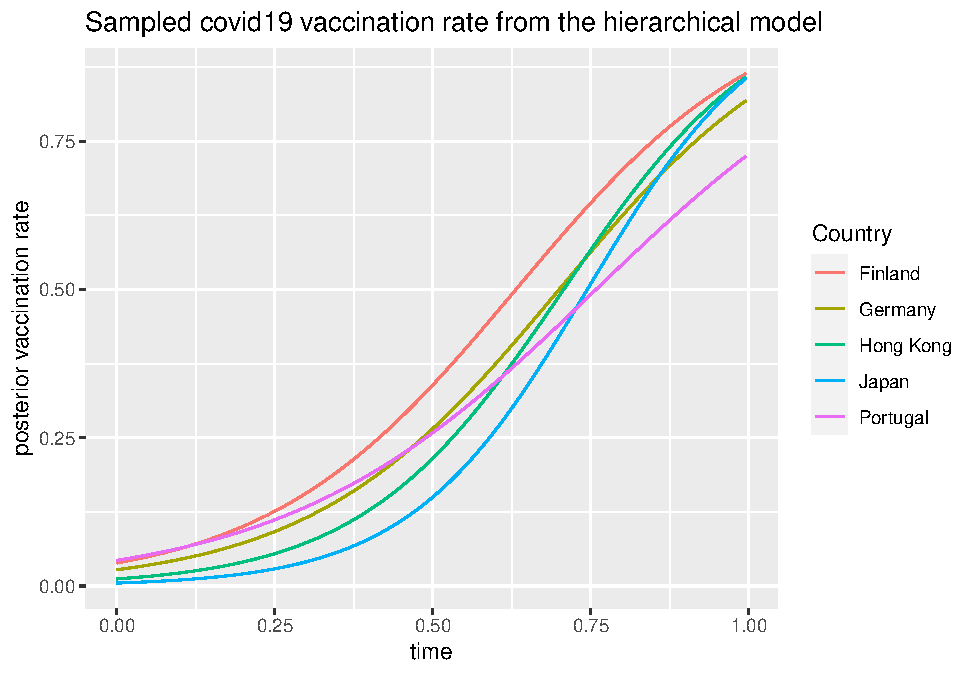
\includegraphics{bda_project_files/figure-latex/unnamed-chunk-17-1.pdf}

With the command \texttt{rstan::stan\_model} we compile our stan models
from a string vector and in the next step with \texttt{rstan::sampling}
we create samples from the models. The given data are the datasets from
section 2. As a warmup phase we use the generous length of \(3000\) and
as a total chain length \(4000\). As the warmup lenght is longer than
half of the chain length we made sure, that the samples are within our
posterior distribution.

\newpage

\hypertarget{convergence-diagnostics-rhat-ess-divergences-and-what-was-done-if-the-convergence-was-not-good-with-the-first-try.}{%
\section{7.Convergence diagnostics (Rhat, ESS, divergences) and what was
done if the convergence was not good with the first
try.}\label{convergence-diagnostics-rhat-ess-divergences-and-what-was-done-if-the-convergence-was-not-good-with-the-first-try.}}

We will use the build in tool from the stan library to analyse the
convergence of our chains.

\begin{Shaded}
\begin{Highlighting}[]
\CommentTok{\#seperate model}
\NormalTok{sum\_seperate }\OtherTok{\textless{}{-}} \FunctionTok{summary}\NormalTok{(model\_separated)}
\FunctionTok{cat}\NormalTok{(}\StringTok{"Rhat of seperate model: }\SpecialCharTok{\textbackslash{}n}\StringTok{"}\NormalTok{)}
\end{Highlighting}
\end{Shaded}

\begin{verbatim}
## Rhat of seperate model:
\end{verbatim}

\begin{Shaded}
\begin{Highlighting}[]
\NormalTok{sum\_seperate}\SpecialCharTok{$}\NormalTok{summary[}\DecValTok{1}\SpecialCharTok{:}\DecValTok{11}\NormalTok{,}\DecValTok{10}\NormalTok{]}
\end{Highlighting}
\end{Shaded}

\begin{verbatim}
##  alpha[1]  alpha[2]  alpha[3]  alpha[4]  alpha[5]   beta[1]   beta[2]   beta[3] 
## 0.9992338 0.9994508 1.0002076 0.9999659 0.9993267 0.9995834 0.9996926 0.9999351 
##   beta[4]   beta[5]     sigma 
## 0.9995020 0.9993671 0.9998387
\end{verbatim}

\begin{Shaded}
\begin{Highlighting}[]
\CommentTok{\#hierarchical}
\NormalTok{sum\_hierarchical }\OtherTok{\textless{}{-}} \FunctionTok{summary}\NormalTok{(model\_hierarchical)}
\FunctionTok{cat}\NormalTok{(}\StringTok{"Rhat of hierarchical model: }\SpecialCharTok{\textbackslash{}n}\StringTok{"}\NormalTok{)}
\end{Highlighting}
\end{Shaded}

\begin{verbatim}
## Rhat of hierarchical model:
\end{verbatim}

\begin{Shaded}
\begin{Highlighting}[]
\NormalTok{sum\_hierarchical}\SpecialCharTok{$}\NormalTok{summary[}\DecValTok{1}\SpecialCharTok{:}\DecValTok{11}\NormalTok{,}\DecValTok{10}\NormalTok{]}
\end{Highlighting}
\end{Shaded}

\begin{verbatim}
##  alpha[1]  alpha[2]  alpha[3]  alpha[4]  alpha[5]   beta[1]   beta[2]   beta[3] 
## 0.9997102 1.0001940 0.9993360 0.9999077 0.9995901 0.9992294 0.9997746 0.9997315 
##   beta[4]   beta[5]     sigma 
## 0.9994987 0.9997845 0.9993087
\end{verbatim}

\[
\begin{aligned}
\hat{R} = \sqrt\frac{\hat{var^*}}{W}
\end{aligned}
\]

R hat is potential scale reduction factor. This value estimates how much
the scale could reduce if N goes infinite. When N approches infinity, R
hat approches 1. If R hat is bigger than 1.01, we should keep sampling.

As we can see here, the \(\hat{R}\) values are less than 1, which means,
that the chains converges. We will now run the ESS analysis, to further
verify, that our \(\hat{R}\) values are trustworthy. As mentioned in
Verteri et al.~2019 @vehtari2019rank, a ESS value above 400 will
indicate that the \(\hat{R}\) value is reliable. We therefore now use
the ESS method from @vehtari2019rank:

\begin{Shaded}
\begin{Highlighting}[]
\FunctionTok{cat}\NormalTok{(}\StringTok{"ESS of seperated model: }\SpecialCharTok{\textbackslash{}n}\StringTok{"}\NormalTok{)}
\end{Highlighting}
\end{Shaded}

\begin{verbatim}
## ESS of seperated model:
\end{verbatim}

\begin{Shaded}
\begin{Highlighting}[]
\NormalTok{sum\_seperate}\SpecialCharTok{$}\NormalTok{summary[}\DecValTok{1}\SpecialCharTok{:}\DecValTok{11}\NormalTok{,}\DecValTok{9}\NormalTok{]}
\end{Highlighting}
\end{Shaded}

\begin{verbatim}
## alpha[1] alpha[2] alpha[3] alpha[4] alpha[5]  beta[1]  beta[2]  beta[3] 
## 8982.082 6175.439 7670.116 5986.019 7997.984 8002.180 7464.720 7988.085 
##  beta[4]  beta[5]    sigma 
## 5576.944 7255.206 7677.715
\end{verbatim}

\begin{Shaded}
\begin{Highlighting}[]
\FunctionTok{cat}\NormalTok{(}\StringTok{"ESS of hiracical model: }\SpecialCharTok{\textbackslash{}n}\StringTok{"}\NormalTok{)}
\end{Highlighting}
\end{Shaded}

\begin{verbatim}
## ESS of hiracical model:
\end{verbatim}

\begin{Shaded}
\begin{Highlighting}[]
\NormalTok{sum\_hierarchical}\SpecialCharTok{$}\NormalTok{summary[}\DecValTok{1}\SpecialCharTok{:}\DecValTok{11}\NormalTok{,}\DecValTok{9}\NormalTok{]}
\end{Highlighting}
\end{Shaded}

\begin{verbatim}
## alpha[1] alpha[2] alpha[3] alpha[4] alpha[5]  beta[1]  beta[2]  beta[3] 
## 7565.916 6902.018 8205.637 5614.604 7270.677 8622.069 7543.622 8893.456 
##  beta[4]  beta[5]    sigma 
## 6035.847 9922.472 7517.843
\end{verbatim}

Here we can nicely see, that all ESS values are above 400, which
indicates, that our \(\hat{R}\) values are realiable. We can therefore
conclude, that our chains converged.

\newpage

\hypertarget{posterior-predictive-checks-and-what-was-done-to-improve-the-model.}{%
\section{8. Posterior predictive checks and what was done to improve the
model.}\label{posterior-predictive-checks-and-what-was-done-to-improve-the-model.}}

We want to see if our model works by posterior predictive checking.

\hypertarget{the-posterior-expectations-with-a-90-credible-interval}{%
\subsection{The posterior expectations with a 90\% credible
interval}\label{the-posterior-expectations-with-a-90-credible-interval}}

\begin{Shaded}
\begin{Highlighting}[]
\CommentTok{\#the posterior expectation for parameter with a 90\% credible interval}
\NormalTok{mu\_pred\_interval}\OtherTok{\textless{}{-}}\ControlFlowTok{function}\NormalTok{(data, prob)\{}
\NormalTok{degree }\OtherTok{=} \FunctionTok{length}\NormalTok{(data)}\SpecialCharTok{{-}}\DecValTok{1}
\NormalTok{mu }\OtherTok{=} \FunctionTok{mean}\NormalTok{(data)}
\NormalTok{sig }\OtherTok{=} \FunctionTok{sqrt}\NormalTok{(}\FunctionTok{var}\NormalTok{(data)}\SpecialCharTok{*}\NormalTok{(}\DecValTok{1}\SpecialCharTok{+}\DecValTok{1}\SpecialCharTok{/}\FunctionTok{length}\NormalTok{(data)))}
\NormalTok{error }\OtherTok{=} \FunctionTok{qt}\NormalTok{(prob}\SpecialCharTok{+}\NormalTok{(}\DecValTok{1}\SpecialCharTok{{-}}\NormalTok{prob)}\SpecialCharTok{/}\DecValTok{2}\NormalTok{,degree)}\SpecialCharTok{*}\NormalTok{sig}
\NormalTok{lower }\OtherTok{=}\NormalTok{ mu }\SpecialCharTok{{-}}\NormalTok{error}
\NormalTok{upper }\OtherTok{=}\NormalTok{ mu }\SpecialCharTok{+}\NormalTok{error}
\NormalTok{interval }\OtherTok{=} \FunctionTok{c}\NormalTok{(lower,upper)}
\FunctionTok{return}\NormalTok{(interval)}
\NormalTok{\}}
\end{Highlighting}
\end{Shaded}

For example, let's see the vaccination rate in Finland on the random
data point 200 in \([1,222]\).

\begin{Shaded}
\begin{Highlighting}[]
\CommentTok{\#seperate model}
\NormalTok{a\_s }\OtherTok{=} \FunctionTok{mu\_pred\_interval}\NormalTok{(}\AttributeTok{data =}\NormalTok{ fit\_sm}\SpecialCharTok{$}\NormalTok{mu[,}\DecValTok{1}\NormalTok{,}\DecValTok{200}\NormalTok{], }\AttributeTok{prob =} \FloatTok{0.90}\NormalTok{)}
\FunctionTok{cat}\NormalTok{(}\StringTok{\textquotesingle{}Actual vaccination rate: \textquotesingle{}}\NormalTok{,finland}\SpecialCharTok{$}\NormalTok{Y[}\DecValTok{200}\NormalTok{],}\StringTok{\textquotesingle{}}\SpecialCharTok{\textbackslash{}n}\StringTok{\textquotesingle{}}\NormalTok{)}
\end{Highlighting}
\end{Shaded}

\begin{verbatim}
## Actual vaccination rate:  0.7301881
\end{verbatim}

\begin{Shaded}
\begin{Highlighting}[]
\FunctionTok{cat}\NormalTok{(}\StringTok{\textquotesingle{}Credible interval of predicted vaccination rate in seperated model: \textquotesingle{}}\NormalTok{,}
\NormalTok{    a\_s,}\StringTok{\textquotesingle{}}\SpecialCharTok{\textbackslash{}n}\StringTok{\textquotesingle{}}\NormalTok{)}
\end{Highlighting}
\end{Shaded}

\begin{verbatim}
## Credible interval of predicted vaccination rate in seperated model:  0.7841126 0.8000001
\end{verbatim}

\begin{Shaded}
\begin{Highlighting}[]
\CommentTok{\#hierarchical model}
\NormalTok{a\_h }\OtherTok{=} \FunctionTok{mu\_pred\_interval}\NormalTok{(}\AttributeTok{data =}\NormalTok{ fit\_hm}\SpecialCharTok{$}\NormalTok{ypred[,}\DecValTok{1}\NormalTok{,}\DecValTok{200}\NormalTok{], }\AttributeTok{prob =} \FloatTok{0.90}\NormalTok{)}
\FunctionTok{cat}\NormalTok{(}\StringTok{\textquotesingle{}Actual vaccination rate: \textquotesingle{}}\NormalTok{,finland}\SpecialCharTok{$}\NormalTok{Y[}\DecValTok{200}\NormalTok{],}\StringTok{\textquotesingle{}}\SpecialCharTok{\textbackslash{}n}\StringTok{\textquotesingle{}}\NormalTok{)}
\end{Highlighting}
\end{Shaded}

\begin{verbatim}
## Actual vaccination rate:  0.7301881
\end{verbatim}

\begin{Shaded}
\begin{Highlighting}[]
\FunctionTok{cat}\NormalTok{(}\StringTok{\textquotesingle{}Credible interval of predicted vaccination rate in hierarchical model: \textquotesingle{}}\NormalTok{,}
\NormalTok{    a\_h,}\StringTok{\textquotesingle{}}\SpecialCharTok{\textbackslash{}n}\StringTok{\textquotesingle{}}\NormalTok{)}
\end{Highlighting}
\end{Shaded}

\begin{verbatim}
## Credible interval of predicted vaccination rate in hierarchical model:  0.7243148 0.8615208
\end{verbatim}

In seperate model, the credible interval for \(\mu\) in datapoint 200
which is \([0.7843056, 0.7995294]\) doesn't include the actual
vaccination rate 0.7301881. However, in hierarchical model, the credible
interval \([0.7232421, 0.8609337]\) includes actual vaccination rate.

\hypertarget{visual-comparisions}{%
\subsection{Visual comparisions}\label{visual-comparisions}}

In posterior expectations with a 90\% credible interval, we checked in
one datapoint. We will now also show, how close our modeling is, when
compared to the original data in overall whole data points. We choose
for this a visual approach down below.

\hypertarget{seperated-model-1}{%
\subsubsection{Seperated model}\label{seperated-model-1}}

\begin{Shaded}
\begin{Highlighting}[]
\NormalTok{finland\_mu }\OtherTok{\textless{}{-}} \FunctionTok{c}\NormalTok{()}
\ControlFlowTok{for}\NormalTok{(i }\ControlFlowTok{in} \DecValTok{3001}\SpecialCharTok{:}\DecValTok{4000}\NormalTok{)\{}
\NormalTok{    finland\_mu }\OtherTok{\textless{}{-}} \FunctionTok{c}\NormalTok{(finland\_mu, fit\_sm}\SpecialCharTok{$}\NormalTok{ypred[i,}\DecValTok{1}\NormalTok{,}\DecValTok{1}\SpecialCharTok{:}\DecValTok{222}\NormalTok{])}
\NormalTok{\}}
\NormalTok{Y\_s }\OtherTok{=} \FunctionTok{c}\NormalTok{(finland\_mu,finland}\SpecialCharTok{$}\NormalTok{Y)}
\NormalTok{names }\OtherTok{=} \FunctionTok{c}\NormalTok{(}\FunctionTok{rep}\NormalTok{(}\FunctionTok{c}\NormalTok{(}\StringTok{"A\_Model"}\NormalTok{), }\AttributeTok{times =} \DecValTok{222}\SpecialCharTok{*}\DecValTok{1000}\NormalTok{, }
              \AttributeTok{length.out =} \ConstantTok{NA}\NormalTok{, }\AttributeTok{each =} \DecValTok{1}\NormalTok{), finland}\SpecialCharTok{$}\NormalTok{Country)}
\NormalTok{result\_s }\OtherTok{=} \FunctionTok{data.frame}\NormalTok{(}\AttributeTok{Country=}\NormalTok{names,}\AttributeTok{X=}\FunctionTok{rep}\NormalTok{(total}\SpecialCharTok{$}\NormalTok{X[}\DecValTok{1}\SpecialCharTok{:}\DecValTok{222}\NormalTok{], }
                      \AttributeTok{times =}\DecValTok{1001}\NormalTok{, }\AttributeTok{length.out =} \ConstantTok{NA}\NormalTok{, }\AttributeTok{each =} \DecValTok{1}\NormalTok{),}\AttributeTok{Y=}\NormalTok{Y\_s)}
\FunctionTok{ggplot}\NormalTok{(}\AttributeTok{data =}\NormalTok{ result\_s, }\FunctionTok{aes}\NormalTok{(}\AttributeTok{x =}\NormalTok{X, }\AttributeTok{y =}\NormalTok{ Y, }\AttributeTok{color =}\NormalTok{ Country)) }\SpecialCharTok{+}
    \FunctionTok{geom\_line}\NormalTok{() }\SpecialCharTok{+}
    \FunctionTok{ggtitle}\NormalTok{(}\StringTok{"Seperate modeled means and accual data for Finland"}\NormalTok{) }\SpecialCharTok{+}
    \FunctionTok{xlab}\NormalTok{(}\StringTok{"time"}\NormalTok{) }\SpecialCharTok{+} \FunctionTok{ylab}\NormalTok{(}\StringTok{"vaccination rate"}\NormalTok{)}
\end{Highlighting}
\end{Shaded}

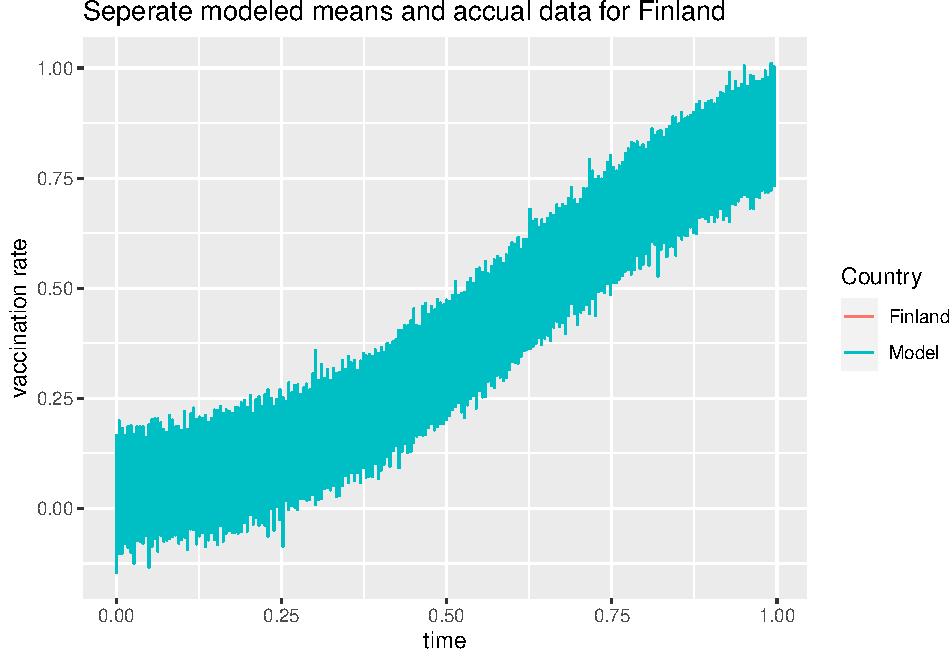
\includegraphics{bda_project_files/figure-latex/unnamed-chunk-25-1.pdf}

\begin{Shaded}
\begin{Highlighting}[]
\CommentTok{\#germany}
\NormalTok{germany\_mu }\OtherTok{\textless{}{-}} \FunctionTok{c}\NormalTok{()}
\ControlFlowTok{for}\NormalTok{(i }\ControlFlowTok{in} \DecValTok{3001}\SpecialCharTok{:}\DecValTok{4000}\NormalTok{)\{}
\NormalTok{    germany\_mu }\OtherTok{\textless{}{-}} \FunctionTok{c}\NormalTok{(germany\_mu, fit\_sm}\SpecialCharTok{$}\NormalTok{ypred[i,}\DecValTok{2}\NormalTok{,}\DecValTok{1}\SpecialCharTok{:}\DecValTok{222}\NormalTok{])}
\NormalTok{\}}
\NormalTok{Y\_s }\OtherTok{=} \FunctionTok{c}\NormalTok{(germany\_mu,germany}\SpecialCharTok{$}\NormalTok{Y)}
\NormalTok{names }\OtherTok{=} \FunctionTok{c}\NormalTok{(}\FunctionTok{rep}\NormalTok{(}\FunctionTok{c}\NormalTok{(}\StringTok{"A\_Model"}\NormalTok{), }\AttributeTok{times =} \DecValTok{222}\SpecialCharTok{*}\DecValTok{1000}\NormalTok{, }
              \AttributeTok{length.out =} \ConstantTok{NA}\NormalTok{, }\AttributeTok{each =} \DecValTok{1}\NormalTok{), germany}\SpecialCharTok{$}\NormalTok{Country)}
\NormalTok{result\_s }\OtherTok{=} \FunctionTok{data.frame}\NormalTok{(}\AttributeTok{Country=}\NormalTok{names,}\AttributeTok{X=}\FunctionTok{rep}\NormalTok{(total}\SpecialCharTok{$}\NormalTok{X[}\DecValTok{1}\SpecialCharTok{:}\DecValTok{222}\NormalTok{], }
                      \AttributeTok{times =}\DecValTok{1001}\NormalTok{, }\AttributeTok{length.out =} \ConstantTok{NA}\NormalTok{, }\AttributeTok{each =} \DecValTok{1}\NormalTok{),}\AttributeTok{Y=}\NormalTok{Y\_s)}
\FunctionTok{ggplot}\NormalTok{(}\AttributeTok{data =}\NormalTok{ result\_s, }\FunctionTok{aes}\NormalTok{(}\AttributeTok{x =}\NormalTok{X, }\AttributeTok{y =}\NormalTok{ Y, }\AttributeTok{color =}\NormalTok{ Country)) }\SpecialCharTok{+}
    \FunctionTok{geom\_line}\NormalTok{() }\SpecialCharTok{+}
    \FunctionTok{ggtitle}\NormalTok{(}\StringTok{"Seperate modeled means and accual data for Germany"}\NormalTok{) }\SpecialCharTok{+}
    \FunctionTok{xlab}\NormalTok{(}\StringTok{"time"}\NormalTok{) }\SpecialCharTok{+} \FunctionTok{ylab}\NormalTok{(}\StringTok{"vaccination rate"}\NormalTok{)}
\end{Highlighting}
\end{Shaded}

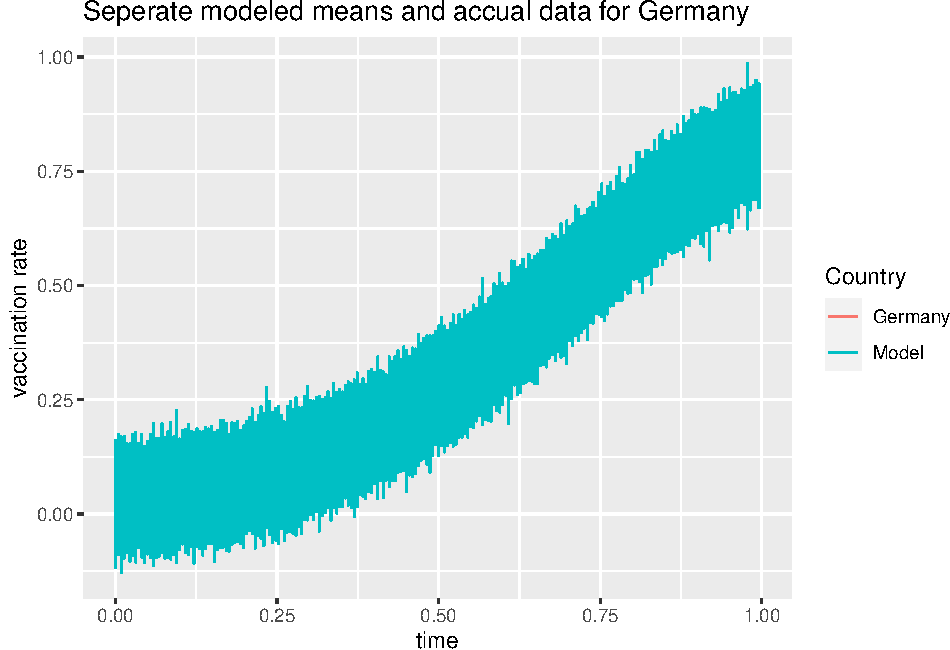
\includegraphics{bda_project_files/figure-latex/unnamed-chunk-26-1.pdf}

\begin{Shaded}
\begin{Highlighting}[]
\CommentTok{\#portugal}
\NormalTok{portugal\_mu }\OtherTok{\textless{}{-}} \FunctionTok{c}\NormalTok{()}
\ControlFlowTok{for}\NormalTok{(i }\ControlFlowTok{in} \DecValTok{3001}\SpecialCharTok{:}\DecValTok{4000}\NormalTok{)\{}
\NormalTok{    portugal\_mu }\OtherTok{\textless{}{-}} \FunctionTok{c}\NormalTok{(portugal\_mu, fit\_sm}\SpecialCharTok{$}\NormalTok{ypred[i,}\DecValTok{3}\NormalTok{,}\DecValTok{1}\SpecialCharTok{:}\DecValTok{222}\NormalTok{])}
\NormalTok{\}}
\NormalTok{Y\_s }\OtherTok{=} \FunctionTok{c}\NormalTok{(portugal\_mu,portugal}\SpecialCharTok{$}\NormalTok{Y)}
\NormalTok{names }\OtherTok{=} \FunctionTok{c}\NormalTok{(}\FunctionTok{rep}\NormalTok{(}\FunctionTok{c}\NormalTok{(}\StringTok{"A\_Model"}\NormalTok{), }\AttributeTok{times =} \DecValTok{222}\SpecialCharTok{*}\DecValTok{1000}\NormalTok{, }
              \AttributeTok{length.out =} \ConstantTok{NA}\NormalTok{, }\AttributeTok{each =} \DecValTok{1}\NormalTok{), portugal}\SpecialCharTok{$}\NormalTok{Country)}
\NormalTok{result\_s }\OtherTok{=} \FunctionTok{data.frame}\NormalTok{(}\AttributeTok{Country=}\NormalTok{names,}\AttributeTok{X=}\FunctionTok{rep}\NormalTok{(total}\SpecialCharTok{$}\NormalTok{X[}\DecValTok{1}\SpecialCharTok{:}\DecValTok{222}\NormalTok{], }
                      \AttributeTok{times =}\DecValTok{1001}\NormalTok{, }\AttributeTok{length.out =} \ConstantTok{NA}\NormalTok{, }\AttributeTok{each =} \DecValTok{1}\NormalTok{),}\AttributeTok{Y=}\NormalTok{Y\_s)}
\FunctionTok{ggplot}\NormalTok{(}\AttributeTok{data =}\NormalTok{ result\_s, }\FunctionTok{aes}\NormalTok{(}\AttributeTok{x =}\NormalTok{X, }\AttributeTok{y =}\NormalTok{ Y, }\AttributeTok{color =}\NormalTok{ Country)) }\SpecialCharTok{+}
    \FunctionTok{geom\_line}\NormalTok{() }\SpecialCharTok{+}
    \FunctionTok{ggtitle}\NormalTok{(}\StringTok{"Seperate modeled means and accual data for Portugal"}\NormalTok{) }\SpecialCharTok{+}
    \FunctionTok{xlab}\NormalTok{(}\StringTok{"time"}\NormalTok{) }\SpecialCharTok{+} \FunctionTok{ylab}\NormalTok{(}\StringTok{"vaccination rate"}\NormalTok{)}
\end{Highlighting}
\end{Shaded}

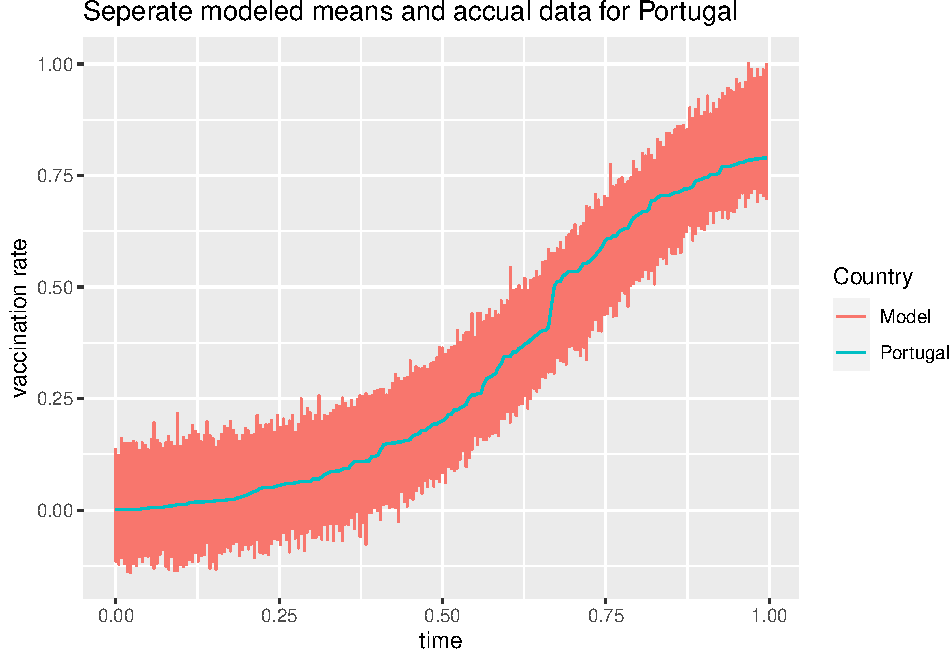
\includegraphics{bda_project_files/figure-latex/unnamed-chunk-27-1.pdf}

\begin{Shaded}
\begin{Highlighting}[]
\CommentTok{\#hongkong}
\NormalTok{hongkong\_mu }\OtherTok{\textless{}{-}} \FunctionTok{c}\NormalTok{()}
\ControlFlowTok{for}\NormalTok{(i }\ControlFlowTok{in} \DecValTok{3001}\SpecialCharTok{:}\DecValTok{4000}\NormalTok{)\{}
\NormalTok{    hongkong\_mu }\OtherTok{\textless{}{-}} \FunctionTok{c}\NormalTok{(hongkong\_mu, fit\_sm}\SpecialCharTok{$}\NormalTok{ypred[i,}\DecValTok{4}\NormalTok{,}\DecValTok{1}\SpecialCharTok{:}\DecValTok{222}\NormalTok{])}
\NormalTok{\}}
\NormalTok{Y\_s }\OtherTok{=} \FunctionTok{c}\NormalTok{(hongkong\_mu,hongkong}\SpecialCharTok{$}\NormalTok{Y)}
\NormalTok{names }\OtherTok{=} \FunctionTok{c}\NormalTok{(}\FunctionTok{rep}\NormalTok{(}\FunctionTok{c}\NormalTok{(}\StringTok{"A\_Model"}\NormalTok{), }\AttributeTok{times =} \DecValTok{222}\SpecialCharTok{*}\DecValTok{1000}\NormalTok{, }
              \AttributeTok{length.out =} \ConstantTok{NA}\NormalTok{, }\AttributeTok{each =} \DecValTok{1}\NormalTok{), hongkong}\SpecialCharTok{$}\NormalTok{Country)}
\NormalTok{result\_s }\OtherTok{=} \FunctionTok{data.frame}\NormalTok{(}\AttributeTok{Country=}\NormalTok{names,}\AttributeTok{X=}\FunctionTok{rep}\NormalTok{(total}\SpecialCharTok{$}\NormalTok{X[}\DecValTok{1}\SpecialCharTok{:}\DecValTok{222}\NormalTok{],}
                      \AttributeTok{times =}\DecValTok{1001}\NormalTok{, }\AttributeTok{length.out =} \ConstantTok{NA}\NormalTok{, }\AttributeTok{each =} \DecValTok{1}\NormalTok{),}\AttributeTok{Y=}\NormalTok{Y\_s)}
\FunctionTok{ggplot}\NormalTok{(}\AttributeTok{data =}\NormalTok{ result\_s, }\FunctionTok{aes}\NormalTok{(}\AttributeTok{x =}\NormalTok{X, }\AttributeTok{y =}\NormalTok{ Y, }\AttributeTok{color =}\NormalTok{ Country)) }\SpecialCharTok{+}
    \FunctionTok{geom\_line}\NormalTok{() }\SpecialCharTok{+}
    \FunctionTok{ggtitle}\NormalTok{(}\StringTok{"Seperate modeled means and accual data for Hongkong"}\NormalTok{) }\SpecialCharTok{+}
    \FunctionTok{xlab}\NormalTok{(}\StringTok{"time"}\NormalTok{) }\SpecialCharTok{+} \FunctionTok{ylab}\NormalTok{(}\StringTok{"vaccination rate"}\NormalTok{)}
\end{Highlighting}
\end{Shaded}

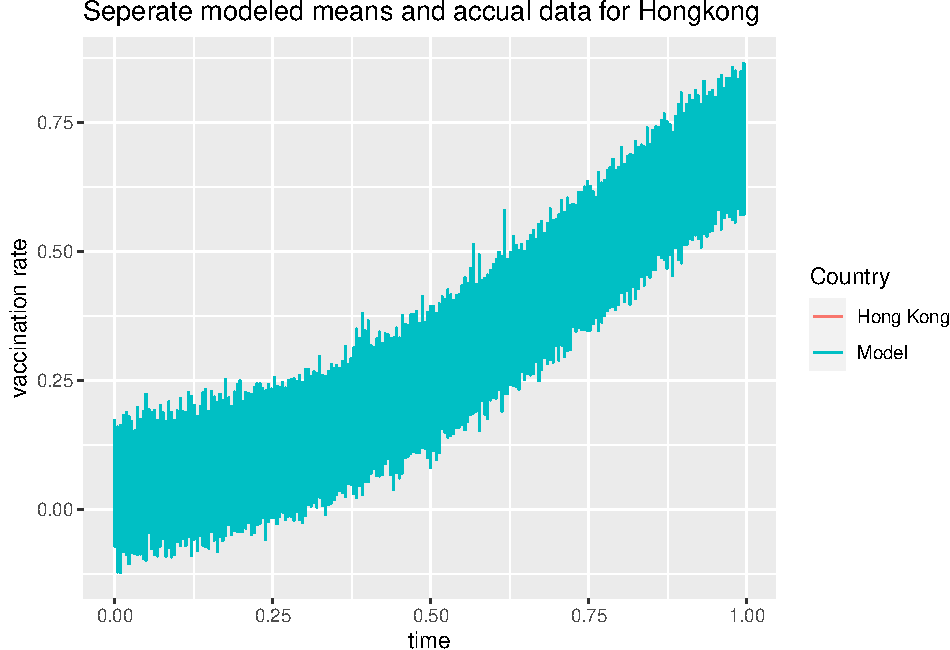
\includegraphics{bda_project_files/figure-latex/unnamed-chunk-28-1.pdf}

\begin{Shaded}
\begin{Highlighting}[]
\CommentTok{\#japan}
\NormalTok{japan\_mu }\OtherTok{\textless{}{-}} \FunctionTok{c}\NormalTok{()}
\ControlFlowTok{for}\NormalTok{(i }\ControlFlowTok{in} \DecValTok{3001}\SpecialCharTok{:}\DecValTok{4000}\NormalTok{)\{}
\NormalTok{    japan\_mu }\OtherTok{\textless{}{-}} \FunctionTok{c}\NormalTok{(japan\_mu, fit\_sm}\SpecialCharTok{$}\NormalTok{ypred[i,}\DecValTok{5}\NormalTok{,}\DecValTok{1}\SpecialCharTok{:}\DecValTok{222}\NormalTok{])}
\NormalTok{\}}
\NormalTok{Y\_s }\OtherTok{=} \FunctionTok{c}\NormalTok{(japan\_mu,japan}\SpecialCharTok{$}\NormalTok{Y)}
\NormalTok{names }\OtherTok{=} \FunctionTok{c}\NormalTok{(}\FunctionTok{rep}\NormalTok{(}\FunctionTok{c}\NormalTok{(}\StringTok{"A\_Model"}\NormalTok{), }\AttributeTok{times =} \DecValTok{222}\SpecialCharTok{*}\DecValTok{1000}\NormalTok{, }
              \AttributeTok{length.out =} \ConstantTok{NA}\NormalTok{, }\AttributeTok{each =} \DecValTok{1}\NormalTok{), japan}\SpecialCharTok{$}\NormalTok{Country)}
\NormalTok{result\_s }\OtherTok{=} \FunctionTok{data.frame}\NormalTok{(}\AttributeTok{Country=}\NormalTok{names,}\AttributeTok{X=}\FunctionTok{rep}\NormalTok{(total}\SpecialCharTok{$}\NormalTok{X[}\DecValTok{1}\SpecialCharTok{:}\DecValTok{222}\NormalTok{],}
                      \AttributeTok{times =}\DecValTok{1001}\NormalTok{, }\AttributeTok{length.out =} \ConstantTok{NA}\NormalTok{, }\AttributeTok{each =} \DecValTok{1}\NormalTok{),}\AttributeTok{Y=}\NormalTok{Y\_s)}
\FunctionTok{ggplot}\NormalTok{(}\AttributeTok{data =}\NormalTok{ result\_s, }\FunctionTok{aes}\NormalTok{(}\AttributeTok{x =}\NormalTok{X, }\AttributeTok{y =}\NormalTok{ Y, }\AttributeTok{color =}\NormalTok{ Country)) }\SpecialCharTok{+}
    \FunctionTok{geom\_line}\NormalTok{() }\SpecialCharTok{+}
    \FunctionTok{ggtitle}\NormalTok{(}\StringTok{"Seperate modeled means and accual data for Japan"}\NormalTok{) }\SpecialCharTok{+}
    \FunctionTok{xlab}\NormalTok{(}\StringTok{"time"}\NormalTok{) }\SpecialCharTok{+} \FunctionTok{ylab}\NormalTok{(}\StringTok{"vaccination rate"}\NormalTok{)}
\end{Highlighting}
\end{Shaded}

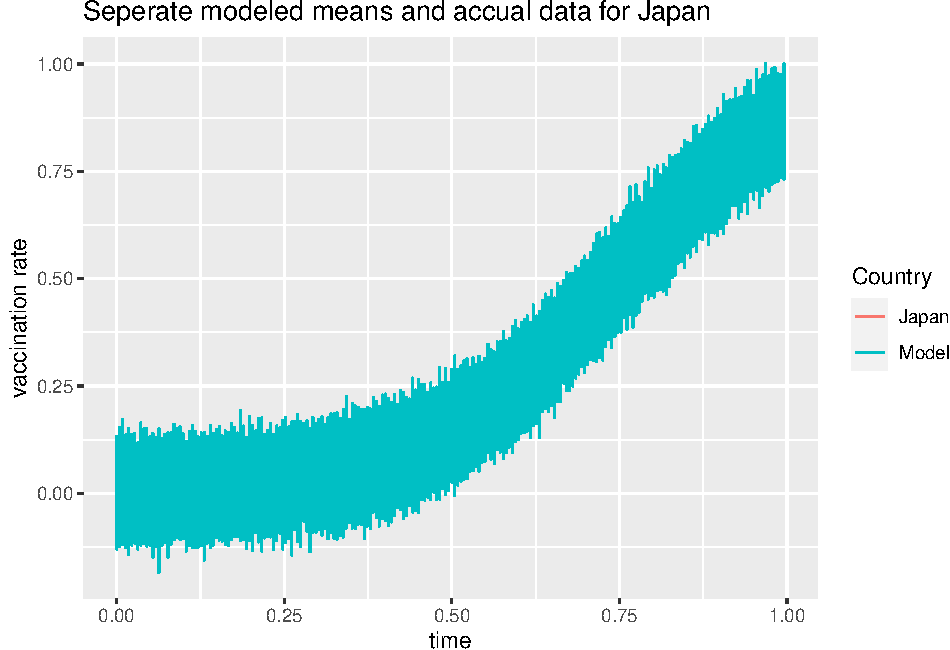
\includegraphics{bda_project_files/figure-latex/unnamed-chunk-29-1.pdf}

\hypertarget{hirachical-model-1}{%
\subsubsection{Hirachical Model}\label{hirachical-model-1}}

\begin{Shaded}
\begin{Highlighting}[]
\NormalTok{finland\_mu }\OtherTok{\textless{}{-}} \FunctionTok{c}\NormalTok{()}
\ControlFlowTok{for}\NormalTok{(i }\ControlFlowTok{in} \DecValTok{3001}\SpecialCharTok{:}\DecValTok{4000}\NormalTok{)\{}
\NormalTok{    finland\_mu }\OtherTok{\textless{}{-}} \FunctionTok{c}\NormalTok{(finland\_mu, fit\_hm}\SpecialCharTok{$}\NormalTok{ypred[i,}\DecValTok{1}\NormalTok{,}\DecValTok{1}\SpecialCharTok{:}\DecValTok{222}\NormalTok{])}
\NormalTok{\}}
\NormalTok{Y\_s }\OtherTok{=} \FunctionTok{c}\NormalTok{(finland\_mu,finland}\SpecialCharTok{$}\NormalTok{Y)}
\NormalTok{names }\OtherTok{=} \FunctionTok{c}\NormalTok{(}\FunctionTok{rep}\NormalTok{(}\FunctionTok{c}\NormalTok{(}\StringTok{"A\_Model"}\NormalTok{), }\AttributeTok{times =} \DecValTok{222}\SpecialCharTok{*}\DecValTok{1000}\NormalTok{,}
              \AttributeTok{length.out =} \ConstantTok{NA}\NormalTok{, }\AttributeTok{each =} \DecValTok{1}\NormalTok{), finland}\SpecialCharTok{$}\NormalTok{Country)}
\NormalTok{result\_s }\OtherTok{=} \FunctionTok{data.frame}\NormalTok{(}\AttributeTok{Country=}\NormalTok{names,}\AttributeTok{X=}\FunctionTok{rep}\NormalTok{(total}\SpecialCharTok{$}\NormalTok{X[}\DecValTok{1}\SpecialCharTok{:}\DecValTok{222}\NormalTok{], }
                      \AttributeTok{times =}\DecValTok{1001}\NormalTok{, }\AttributeTok{length.out =} \ConstantTok{NA}\NormalTok{, }\AttributeTok{each =} \DecValTok{1}\NormalTok{),}\AttributeTok{Y=}\NormalTok{Y\_s)}
\FunctionTok{ggplot}\NormalTok{(}\AttributeTok{data =}\NormalTok{ result\_s, }\FunctionTok{aes}\NormalTok{(}\AttributeTok{x =}\NormalTok{X, }\AttributeTok{y =}\NormalTok{ Y, }\AttributeTok{color =}\NormalTok{ Country)) }\SpecialCharTok{+}
    \FunctionTok{geom\_line}\NormalTok{() }\SpecialCharTok{+}
    \FunctionTok{ggtitle}\NormalTok{(}\StringTok{"Hierarchical modeled means and accual data for Finland"}\NormalTok{) }\SpecialCharTok{+}
    \FunctionTok{xlab}\NormalTok{(}\StringTok{"time"}\NormalTok{) }\SpecialCharTok{+} \FunctionTok{ylab}\NormalTok{(}\StringTok{"vaccination rate"}\NormalTok{)}
\end{Highlighting}
\end{Shaded}

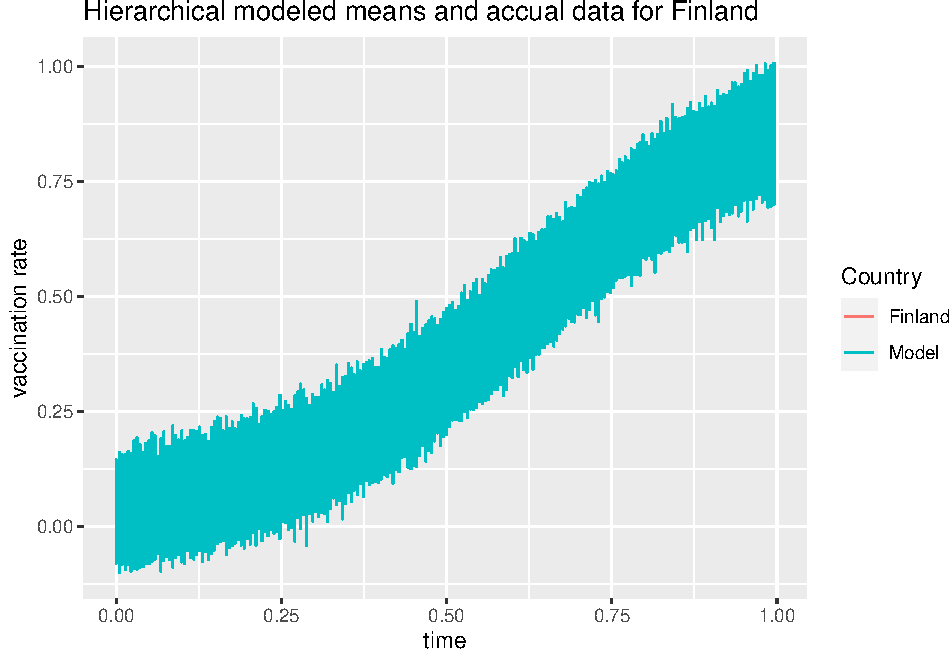
\includegraphics{bda_project_files/figure-latex/unnamed-chunk-30-1.pdf}

\begin{Shaded}
\begin{Highlighting}[]
\CommentTok{\#germany}
\NormalTok{germany\_mu }\OtherTok{\textless{}{-}} \FunctionTok{c}\NormalTok{()}
\ControlFlowTok{for}\NormalTok{(i }\ControlFlowTok{in} \DecValTok{3001}\SpecialCharTok{:}\DecValTok{4000}\NormalTok{)\{}
\NormalTok{    germany\_mu }\OtherTok{\textless{}{-}} \FunctionTok{c}\NormalTok{(germany\_mu, fit\_hm}\SpecialCharTok{$}\NormalTok{ypred[i,}\DecValTok{2}\NormalTok{,}\DecValTok{1}\SpecialCharTok{:}\DecValTok{222}\NormalTok{])}
\NormalTok{\}}
\NormalTok{Y\_s }\OtherTok{=} \FunctionTok{c}\NormalTok{(germany\_mu,germany}\SpecialCharTok{$}\NormalTok{Y)}
\NormalTok{names }\OtherTok{=} \FunctionTok{c}\NormalTok{(}\FunctionTok{rep}\NormalTok{(}\FunctionTok{c}\NormalTok{(}\StringTok{"A\_Model"}\NormalTok{), }\AttributeTok{times =} \DecValTok{222}\SpecialCharTok{*}\DecValTok{1000}\NormalTok{, }
              \AttributeTok{length.out =} \ConstantTok{NA}\NormalTok{, }\AttributeTok{each =} \DecValTok{1}\NormalTok{), germany}\SpecialCharTok{$}\NormalTok{Country)}
\NormalTok{result\_s }\OtherTok{=} \FunctionTok{data.frame}\NormalTok{(}\AttributeTok{Country=}\NormalTok{names,}\AttributeTok{X=}\FunctionTok{rep}\NormalTok{(total}\SpecialCharTok{$}\NormalTok{X[}\DecValTok{1}\SpecialCharTok{:}\DecValTok{222}\NormalTok{], }
                      \AttributeTok{times =}\DecValTok{1001}\NormalTok{, }\AttributeTok{length.out =} \ConstantTok{NA}\NormalTok{, }\AttributeTok{each =} \DecValTok{1}\NormalTok{),}\AttributeTok{Y=}\NormalTok{Y\_s)}
\FunctionTok{ggplot}\NormalTok{(}\AttributeTok{data =}\NormalTok{ result\_s, }\FunctionTok{aes}\NormalTok{(}\AttributeTok{x =}\NormalTok{X, }\AttributeTok{y =}\NormalTok{ Y, }\AttributeTok{color =}\NormalTok{ Country)) }\SpecialCharTok{+}
    \FunctionTok{geom\_line}\NormalTok{() }\SpecialCharTok{+}
    \FunctionTok{ggtitle}\NormalTok{(}\StringTok{"Hierarchical modeled means and accual data for Germany"}\NormalTok{) }\SpecialCharTok{+}
    \FunctionTok{xlab}\NormalTok{(}\StringTok{"time"}\NormalTok{) }\SpecialCharTok{+} \FunctionTok{ylab}\NormalTok{(}\StringTok{"vaccination rate"}\NormalTok{)}
\end{Highlighting}
\end{Shaded}

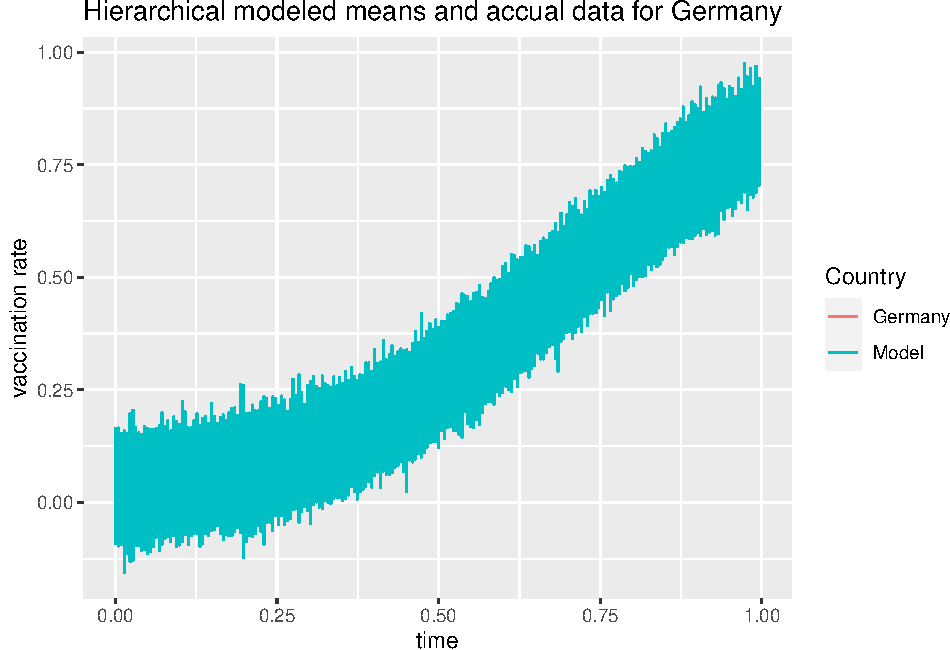
\includegraphics{bda_project_files/figure-latex/unnamed-chunk-31-1.pdf}

\begin{Shaded}
\begin{Highlighting}[]
\CommentTok{\#portugal}
\NormalTok{portugal\_mu }\OtherTok{\textless{}{-}} \FunctionTok{c}\NormalTok{()}
\ControlFlowTok{for}\NormalTok{(i }\ControlFlowTok{in} \DecValTok{3001}\SpecialCharTok{:}\DecValTok{4000}\NormalTok{)\{}
\NormalTok{    portugal\_mu }\OtherTok{\textless{}{-}} \FunctionTok{c}\NormalTok{(portugal\_mu, fit\_hm}\SpecialCharTok{$}\NormalTok{ypred[i,}\DecValTok{3}\NormalTok{,}\DecValTok{1}\SpecialCharTok{:}\DecValTok{222}\NormalTok{])}
\NormalTok{\}}
\NormalTok{Y\_s }\OtherTok{=} \FunctionTok{c}\NormalTok{(portugal\_mu,portugal}\SpecialCharTok{$}\NormalTok{Y)}
\NormalTok{names }\OtherTok{=} \FunctionTok{c}\NormalTok{(}\FunctionTok{rep}\NormalTok{(}\FunctionTok{c}\NormalTok{(}\StringTok{"A\_Model"}\NormalTok{), }\AttributeTok{times =} \DecValTok{222}\SpecialCharTok{*}\DecValTok{1000}\NormalTok{, }
              \AttributeTok{length.out =} \ConstantTok{NA}\NormalTok{, }\AttributeTok{each =} \DecValTok{1}\NormalTok{), portugal}\SpecialCharTok{$}\NormalTok{Country)}
\NormalTok{result\_s }\OtherTok{=} \FunctionTok{data.frame}\NormalTok{(}\AttributeTok{Country=}\NormalTok{names,}\AttributeTok{X=}\FunctionTok{rep}\NormalTok{(total}\SpecialCharTok{$}\NormalTok{X[}\DecValTok{1}\SpecialCharTok{:}\DecValTok{222}\NormalTok{],}
                      \AttributeTok{times =}\DecValTok{1001}\NormalTok{, }\AttributeTok{length.out =} \ConstantTok{NA}\NormalTok{, }\AttributeTok{each =} \DecValTok{1}\NormalTok{),}\AttributeTok{Y=}\NormalTok{Y\_s)}
\FunctionTok{ggplot}\NormalTok{(}\AttributeTok{data =}\NormalTok{ result\_s, }\FunctionTok{aes}\NormalTok{(}\AttributeTok{x =}\NormalTok{X, }\AttributeTok{y =}\NormalTok{ Y, }\AttributeTok{color =}\NormalTok{ Country)) }\SpecialCharTok{+}
    \FunctionTok{geom\_line}\NormalTok{() }\SpecialCharTok{+}
    \FunctionTok{ggtitle}\NormalTok{(}\StringTok{"Hierarchical modeled means and accual data for Portugal"}\NormalTok{) }\SpecialCharTok{+}
    \FunctionTok{xlab}\NormalTok{(}\StringTok{"time"}\NormalTok{) }\SpecialCharTok{+} \FunctionTok{ylab}\NormalTok{(}\StringTok{"vaccination rate"}\NormalTok{)}
\end{Highlighting}
\end{Shaded}

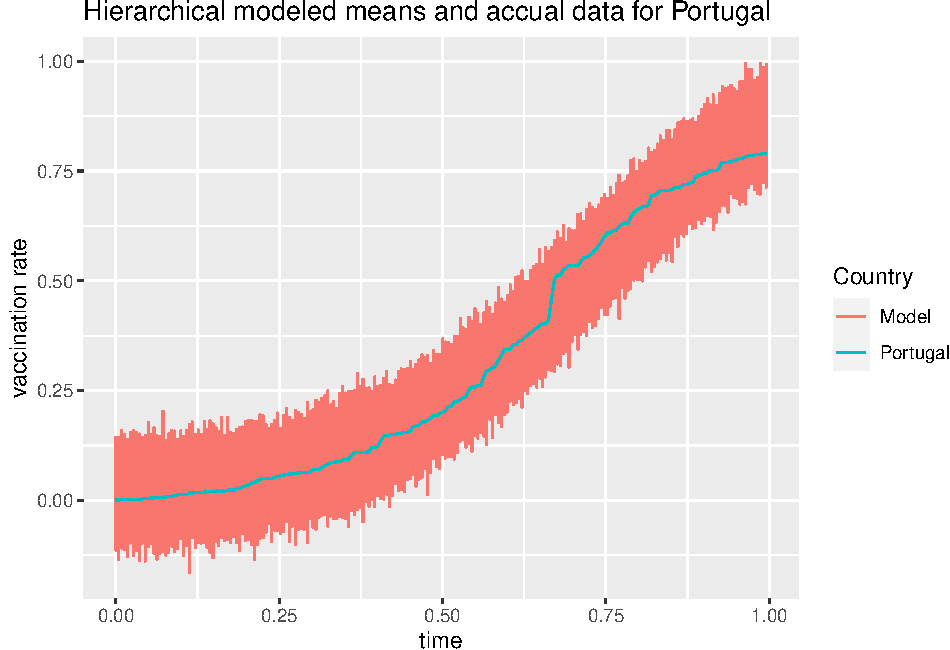
\includegraphics{bda_project_files/figure-latex/unnamed-chunk-32-1.pdf}

\begin{Shaded}
\begin{Highlighting}[]
\CommentTok{\#hongkong}
\NormalTok{hongkong\_mu }\OtherTok{\textless{}{-}} \FunctionTok{c}\NormalTok{()}
\ControlFlowTok{for}\NormalTok{(i }\ControlFlowTok{in} \DecValTok{3001}\SpecialCharTok{:}\DecValTok{4000}\NormalTok{)\{}
\NormalTok{    hongkong\_mu }\OtherTok{\textless{}{-}} \FunctionTok{c}\NormalTok{(hongkong\_mu, fit\_hm}\SpecialCharTok{$}\NormalTok{ypred[i,}\DecValTok{4}\NormalTok{,}\DecValTok{1}\SpecialCharTok{:}\DecValTok{222}\NormalTok{])}
\NormalTok{\}}
\NormalTok{Y\_s }\OtherTok{=} \FunctionTok{c}\NormalTok{(hongkong\_mu,hongkong}\SpecialCharTok{$}\NormalTok{Y)}
\NormalTok{names }\OtherTok{=} \FunctionTok{c}\NormalTok{(}\FunctionTok{rep}\NormalTok{(}\FunctionTok{c}\NormalTok{(}\StringTok{"A\_Model"}\NormalTok{), }\AttributeTok{times =} \DecValTok{222}\SpecialCharTok{*}\DecValTok{1000}\NormalTok{, }
              \AttributeTok{length.out =} \ConstantTok{NA}\NormalTok{, }\AttributeTok{each =} \DecValTok{1}\NormalTok{), hongkong}\SpecialCharTok{$}\NormalTok{Country)}
\NormalTok{result\_s }\OtherTok{=} \FunctionTok{data.frame}\NormalTok{(}\AttributeTok{Country=}\NormalTok{names,}\AttributeTok{X=}\FunctionTok{rep}\NormalTok{(total}\SpecialCharTok{$}\NormalTok{X[}\DecValTok{1}\SpecialCharTok{:}\DecValTok{222}\NormalTok{], }
                      \AttributeTok{times =}\DecValTok{1001}\NormalTok{, }\AttributeTok{length.out =} \ConstantTok{NA}\NormalTok{, }\AttributeTok{each =} \DecValTok{1}\NormalTok{),}\AttributeTok{Y=}\NormalTok{Y\_s)}
\FunctionTok{ggplot}\NormalTok{(}\AttributeTok{data =}\NormalTok{ result\_s, }\FunctionTok{aes}\NormalTok{(}\AttributeTok{x =}\NormalTok{X, }\AttributeTok{y =}\NormalTok{ Y, }\AttributeTok{color =}\NormalTok{ Country)) }\SpecialCharTok{+}
    \FunctionTok{geom\_line}\NormalTok{() }\SpecialCharTok{+}
    \FunctionTok{ggtitle}\NormalTok{(}\StringTok{"Hierarchical modeled means and accual data for Hongkong"}\NormalTok{) }\SpecialCharTok{+}
    \FunctionTok{xlab}\NormalTok{(}\StringTok{"time"}\NormalTok{) }\SpecialCharTok{+} \FunctionTok{ylab}\NormalTok{(}\StringTok{"vaccination rate"}\NormalTok{)}
\end{Highlighting}
\end{Shaded}

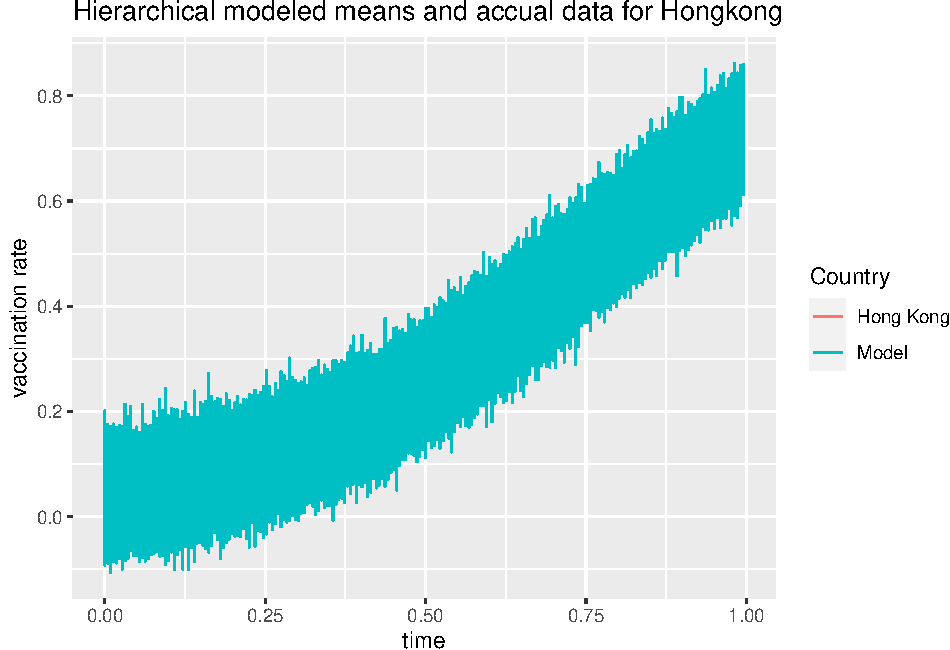
\includegraphics{bda_project_files/figure-latex/unnamed-chunk-33-1.pdf}

\begin{Shaded}
\begin{Highlighting}[]
\CommentTok{\#japan}
\NormalTok{japan\_mu }\OtherTok{\textless{}{-}} \FunctionTok{c}\NormalTok{()}
\ControlFlowTok{for}\NormalTok{(i }\ControlFlowTok{in} \DecValTok{3001}\SpecialCharTok{:}\DecValTok{4000}\NormalTok{)\{}
\NormalTok{    japan\_mu }\OtherTok{\textless{}{-}} \FunctionTok{c}\NormalTok{(japan\_mu, fit\_hm}\SpecialCharTok{$}\NormalTok{ypred[i,}\DecValTok{5}\NormalTok{,}\DecValTok{1}\SpecialCharTok{:}\DecValTok{222}\NormalTok{])}
\NormalTok{\}}
\NormalTok{Y\_s }\OtherTok{=} \FunctionTok{c}\NormalTok{(japan\_mu,japan}\SpecialCharTok{$}\NormalTok{Y)}
\NormalTok{names }\OtherTok{=} \FunctionTok{c}\NormalTok{(}\FunctionTok{rep}\NormalTok{(}\FunctionTok{c}\NormalTok{(}\StringTok{"A\_Model"}\NormalTok{), }\AttributeTok{times =} \DecValTok{222}\SpecialCharTok{*}\DecValTok{1000}\NormalTok{, }
              \AttributeTok{length.out =} \ConstantTok{NA}\NormalTok{, }\AttributeTok{each =} \DecValTok{1}\NormalTok{), japan}\SpecialCharTok{$}\NormalTok{Country)}
\NormalTok{result\_s }\OtherTok{=} \FunctionTok{data.frame}\NormalTok{(}\AttributeTok{Country=}\NormalTok{names,}\AttributeTok{X=}\FunctionTok{rep}\NormalTok{(total}\SpecialCharTok{$}\NormalTok{X[}\DecValTok{1}\SpecialCharTok{:}\DecValTok{222}\NormalTok{], }
                      \AttributeTok{times =}\DecValTok{1001}\NormalTok{, }\AttributeTok{length.out =} \ConstantTok{NA}\NormalTok{, }\AttributeTok{each =} \DecValTok{1}\NormalTok{),}\AttributeTok{Y=}\NormalTok{Y\_s)}
\FunctionTok{ggplot}\NormalTok{(}\AttributeTok{data =}\NormalTok{ result\_s, }\FunctionTok{aes}\NormalTok{(}\AttributeTok{x =}\NormalTok{X, }\AttributeTok{y =}\NormalTok{ Y, }\AttributeTok{color =}\NormalTok{ Country)) }\SpecialCharTok{+}
    \FunctionTok{geom\_line}\NormalTok{() }\SpecialCharTok{+}
    \FunctionTok{ggtitle}\NormalTok{(}\StringTok{"Hierarchical modeled means and accual data for Japan"}\NormalTok{) }\SpecialCharTok{+}
    \FunctionTok{xlab}\NormalTok{(}\StringTok{"time"}\NormalTok{) }\SpecialCharTok{+} \FunctionTok{ylab}\NormalTok{(}\StringTok{"vaccination rate"}\NormalTok{)}
\end{Highlighting}
\end{Shaded}

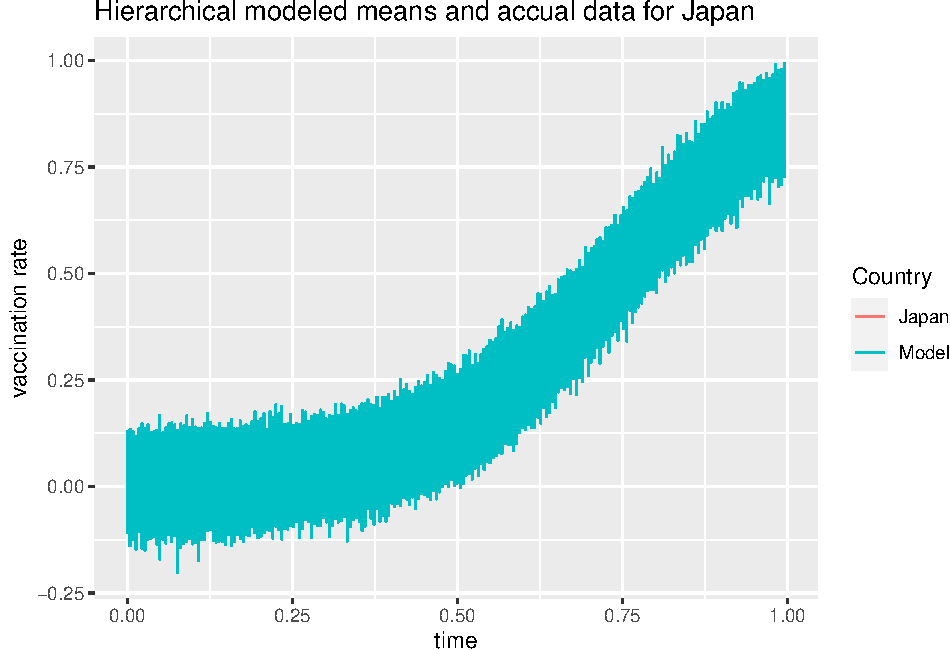
\includegraphics{bda_project_files/figure-latex/unnamed-chunk-34-1.pdf}

\hypertarget{conclusion}{%
\subsubsection{Conclusion}\label{conclusion}}

With those posterior checks we can draw two main conclusions:

\begin{enumerate}
\def\labelenumi{\arabic{enumi}.}
\item
  Our two models are working as they should. They approximate a logistic
  function quite well within our given parameter range. Also the data
  could be a possible sampling from the model, which is a indication,
  that the wished posterior distribution was found and modeled by us in
  Stan
\item
  The sampled variance has also the right size, to ensure, that every
  point from our data could possible be sampled.
\end{enumerate}

The model, as we designed it works and is also suitable for modeling
COVID-19 vaccination rates. In chapter 13 we will further evaluate which
points could be improved.

\newpage

\hypertarget{model-comparison-e.g.-with-loo-cv}{%
\section{9.Model comparison (e.g.~with
LOO-CV)}\label{model-comparison-e.g.-with-loo-cv}}

\begin{Shaded}
\begin{Highlighting}[]
\CommentTok{\#seperate model extract log\_lik}
\NormalTok{l\_like\_s }\OtherTok{\textless{}{-}} \FunctionTok{extract\_log\_lik}\NormalTok{(model\_separated)}
\NormalTok{loo\_s }\OtherTok{\textless{}{-}} \FunctionTok{loo}\NormalTok{(l\_like\_s)}
\end{Highlighting}
\end{Shaded}

\begin{verbatim}
## Warning: Relative effective sample sizes ('r_eff' argument) not specified.
## For models fit with MCMC, the reported PSIS effective sample sizes and 
## MCSE estimates will be over-optimistic.
\end{verbatim}

\begin{Shaded}
\begin{Highlighting}[]
\NormalTok{elpd\_s }\OtherTok{\textless{}{-}}\NormalTok{ loo\_s}\SpecialCharTok{$}\NormalTok{estimates[}\DecValTok{1}\NormalTok{,}\DecValTok{1}\NormalTok{]}

\CommentTok{\#hierarchical model extract log\_lik}
\NormalTok{l\_like\_h }\OtherTok{\textless{}{-}} \FunctionTok{extract\_log\_lik}\NormalTok{(model\_hierarchical)}
\NormalTok{loo\_h }\OtherTok{\textless{}{-}} \FunctionTok{loo}\NormalTok{(l\_like\_h)}
\end{Highlighting}
\end{Shaded}

\begin{verbatim}
## Warning: Relative effective sample sizes ('r_eff' argument) not specified.
## For models fit with MCMC, the reported PSIS effective sample sizes and 
## MCSE estimates will be over-optimistic.
\end{verbatim}

\begin{Shaded}
\begin{Highlighting}[]
\NormalTok{elpd\_h }\OtherTok{\textless{}{-}}\NormalTok{ loo\_h}\SpecialCharTok{$}\NormalTok{estimates[}\DecValTok{1}\NormalTok{,}\DecValTok{1}\NormalTok{]}
\end{Highlighting}
\end{Shaded}

\begin{Shaded}
\begin{Highlighting}[]
\NormalTok{k\_s }\OtherTok{\textless{}{-}}\NormalTok{ loo\_s}\SpecialCharTok{$}\NormalTok{diagnostics}\SpecialCharTok{$}\NormalTok{pareto\_k}
\NormalTok{plot\_s }\OtherTok{\textless{}{-}} \FunctionTok{ggplot}\NormalTok{(}\AttributeTok{data =} \FunctionTok{data.frame}\NormalTok{(}\AttributeTok{x =} \FunctionTok{seq}\NormalTok{(}\DecValTok{1}\NormalTok{,}\FunctionTok{length}\NormalTok{(k\_s)) ,}\AttributeTok{y =}\NormalTok{ k\_s))}
\NormalTok{plot\_s }\SpecialCharTok{+} \FunctionTok{geom\_point}\NormalTok{(}\FunctionTok{aes}\NormalTok{(}\AttributeTok{x =}\NormalTok{ x, }\AttributeTok{y =}\NormalTok{ y, }\AttributeTok{color =} \StringTok{"blue"}\NormalTok{), }\AttributeTok{alpha =} \FloatTok{0.8}\NormalTok{) }\SpecialCharTok{+}
    \FunctionTok{theme\_light}\NormalTok{() }\SpecialCharTok{+}
    \FunctionTok{xlab}\NormalTok{(}\StringTok{""}\NormalTok{) }\SpecialCharTok{+}
    \FunctionTok{ylab}\NormalTok{(}\StringTok{"k{-}value"}\NormalTok{) }\SpecialCharTok{+}
    \FunctionTok{theme}\NormalTok{(}\AttributeTok{legend.position=}\StringTok{"none"}\NormalTok{)}\SpecialCharTok{+}
    \FunctionTok{ggtitle}\NormalTok{(}\StringTok{"K{-}values in seperate model"}\NormalTok{)}
\end{Highlighting}
\end{Shaded}

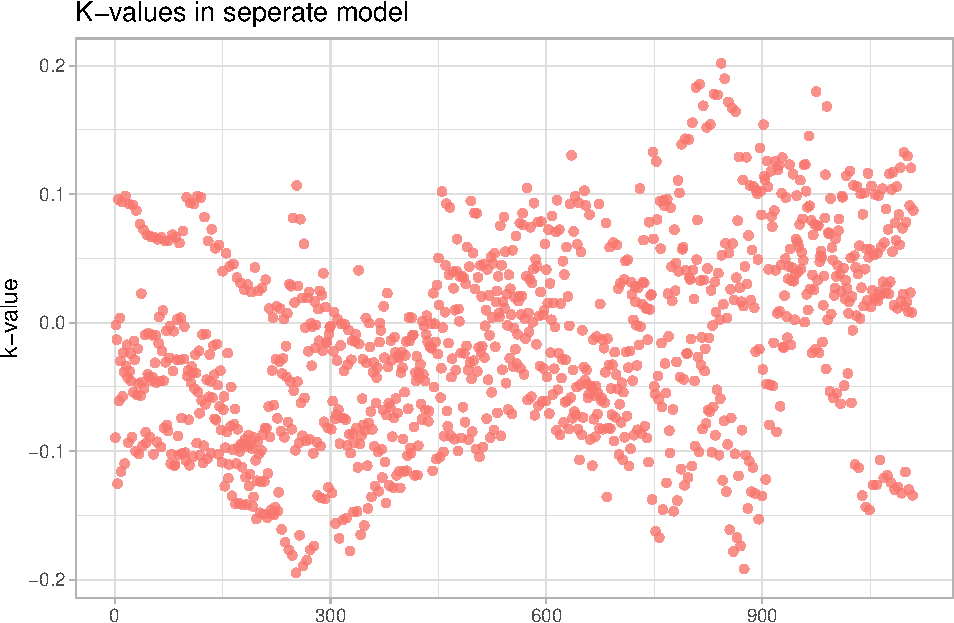
\includegraphics{bda_project_files/figure-latex/unnamed-chunk-36-1.pdf}

\begin{Shaded}
\begin{Highlighting}[]
\NormalTok{k\_h }\OtherTok{\textless{}{-}}\NormalTok{ loo\_h}\SpecialCharTok{$}\NormalTok{diagnostics}\SpecialCharTok{$}\NormalTok{pareto\_k}
\NormalTok{plot\_h }\OtherTok{\textless{}{-}} \FunctionTok{ggplot}\NormalTok{(}\AttributeTok{data =} \FunctionTok{data.frame}\NormalTok{(}\AttributeTok{x =} \FunctionTok{seq}\NormalTok{(}\DecValTok{1}\NormalTok{,}\FunctionTok{length}\NormalTok{(k\_h)) ,}\AttributeTok{y =}\NormalTok{ k\_h))}
\NormalTok{plot\_h }\SpecialCharTok{+} \FunctionTok{geom\_point}\NormalTok{(}\FunctionTok{aes}\NormalTok{(}\AttributeTok{x =}\NormalTok{ x, }\AttributeTok{y =}\NormalTok{ y, }\AttributeTok{color =} \StringTok{"blue"}\NormalTok{), }\AttributeTok{alpha =} \FloatTok{0.8}\NormalTok{) }\SpecialCharTok{+}
    \FunctionTok{theme\_light}\NormalTok{() }\SpecialCharTok{+}
    \FunctionTok{xlab}\NormalTok{(}\StringTok{""}\NormalTok{) }\SpecialCharTok{+}
    \FunctionTok{ylab}\NormalTok{(}\StringTok{"k{-}value"}\NormalTok{) }\SpecialCharTok{+}
    \FunctionTok{theme}\NormalTok{(}\AttributeTok{legend.position=}\StringTok{"none"}\NormalTok{)}\SpecialCharTok{+}
    \FunctionTok{ggtitle}\NormalTok{(}\StringTok{"K{-}values in hierarchical model"}\NormalTok{)}
\end{Highlighting}
\end{Shaded}

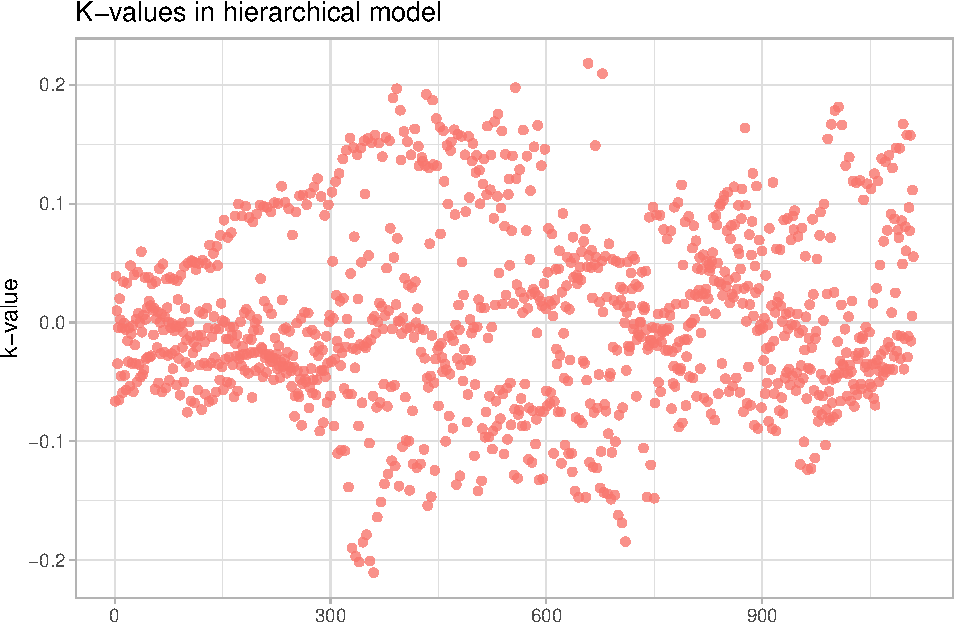
\includegraphics{bda_project_files/figure-latex/unnamed-chunk-37-1.pdf}

\begin{Shaded}
\begin{Highlighting}[]
\FunctionTok{cat}\NormalTok{(}\StringTok{"Maximum k{-}values in seperate model is "}\NormalTok{,}\FunctionTok{max}\NormalTok{(k\_s),}\StringTok{\textquotesingle{}}\SpecialCharTok{\textbackslash{}n}\StringTok{\textquotesingle{}}\NormalTok{)}
\end{Highlighting}
\end{Shaded}

\begin{verbatim}
## Maximum k-values in seperate model is  0.1842326
\end{verbatim}

\begin{Shaded}
\begin{Highlighting}[]
\FunctionTok{cat}\NormalTok{(}\StringTok{"Maximum k{-}values in hierarchical model is "}\NormalTok{,}\FunctionTok{max}\NormalTok{(k\_h),}\StringTok{\textquotesingle{}}\SpecialCharTok{\textbackslash{}n}\StringTok{\textquotesingle{}}\NormalTok{)}
\end{Highlighting}
\end{Shaded}

\begin{verbatim}
## Maximum k-values in hierarchical model is  0.2373332
\end{verbatim}

If the k \textless{} 0.7 we can say that PSIS-LOO estimates are
reliable. Based on this,for seperate model and hierarchical model both,
the \(\hat{k}\)-values are all below 0.5 which are good. Therefore, both
seperate model and hierarchicalmodels are reliable. However, the maximum
\(\hat{k}\)-values in seperate model is 0.216 and the maximum
\(\hat{k}\)-values in hierarchical model is 0.176, so we could say the
hierarchical model is more reliable.

\hypertarget{comparing-psis-loo-estimates}{%
\paragraph{comparing PSIS-LOO
estimates}\label{comparing-psis-loo-estimates}}

\begin{Shaded}
\begin{Highlighting}[]
\FunctionTok{cat}\NormalTok{(}\StringTok{"PSIS{-}LOO estimates in seperate model"}\NormalTok{,elpd\_s,}\StringTok{\textquotesingle{}}\SpecialCharTok{\textbackslash{}n}\StringTok{\textquotesingle{}}\NormalTok{)}
\end{Highlighting}
\end{Shaded}

\begin{verbatim}
## PSIS-LOO estimates in seperate model 1958.753
\end{verbatim}

\begin{Shaded}
\begin{Highlighting}[]
\FunctionTok{cat}\NormalTok{(}\StringTok{"PSIS{-}LOO estimates in hierarchical model"}\NormalTok{,elpd\_h,}\StringTok{\textquotesingle{}}\SpecialCharTok{\textbackslash{}n}\StringTok{\textquotesingle{}}\NormalTok{)}
\end{Highlighting}
\end{Shaded}

\begin{verbatim}
## PSIS-LOO estimates in hierarchical model 1958.806
\end{verbatim}

According to the PSIS-LOO estimate, hierarchical model has slightly
higher value for the PSIS-LOO estimate than seperate model,so we could
choose hierarchical model but still seperate model also have nice score
in PSIS-LOO estimate.

\newpage

\hypertarget{predictive-performance-assessment-if-applicable-e.g.-classification-accuracy-and-evaluation-of-practical-usefulness-of-the-accuracy}{%
\section{10. Predictive performance assessment if applicable
(e.g.~classification accuracy) and evaluation of practical usefulness of
the
accuracy}\label{predictive-performance-assessment-if-applicable-e.g.-classification-accuracy-and-evaluation-of-practical-usefulness-of-the-accuracy}}

We can now evaluate the predictive performance of our model.

\hypertarget{seperate-model}{%
\subsection{Seperate model}\label{seperate-model}}

For the seperated model we have the following numbers:

\begin{Shaded}
\begin{Highlighting}[]
\FunctionTok{qplot}\NormalTok{(fit\_sm}\SpecialCharTok{$}\NormalTok{ypred[,}\DecValTok{1}\NormalTok{,}\DecValTok{223}\NormalTok{], }\AttributeTok{geom=}\StringTok{"histogram"}\NormalTok{) }\SpecialCharTok{+}
    \FunctionTok{xlab}\NormalTok{(}\StringTok{""}\NormalTok{) }\SpecialCharTok{+}
    \FunctionTok{ylab}\NormalTok{(}\StringTok{""}\NormalTok{) }\SpecialCharTok{+}
    \FunctionTok{ggtitle}\NormalTok{(}\StringTok{"Prediction of vaccination rate in close future,Finland"}\NormalTok{)}
\end{Highlighting}
\end{Shaded}

\begin{verbatim}
## `stat_bin()` using `bins = 30`. Pick better value with `binwidth`.
\end{verbatim}

\includegraphics{bda_project_files/figure-latex/unnamed-chunk-40-1.pdf}

\begin{Shaded}
\begin{Highlighting}[]
\FunctionTok{qplot}\NormalTok{(fit\_sm}\SpecialCharTok{$}\NormalTok{ypred[,}\DecValTok{2}\NormalTok{,}\DecValTok{223}\NormalTok{], }\AttributeTok{geom=}\StringTok{"histogram"}\NormalTok{) }\SpecialCharTok{+}
    \FunctionTok{xlab}\NormalTok{(}\StringTok{""}\NormalTok{) }\SpecialCharTok{+}
    \FunctionTok{ylab}\NormalTok{(}\StringTok{""}\NormalTok{) }\SpecialCharTok{+}
    \FunctionTok{ggtitle}\NormalTok{(}\StringTok{"Prediction of vaccination rate in close future, Germany"}\NormalTok{)}
\end{Highlighting}
\end{Shaded}

\begin{verbatim}
## `stat_bin()` using `bins = 30`. Pick better value with `binwidth`.
\end{verbatim}

\includegraphics{bda_project_files/figure-latex/unnamed-chunk-41-1.pdf}

\begin{Shaded}
\begin{Highlighting}[]
\FunctionTok{qplot}\NormalTok{(fit\_sm}\SpecialCharTok{$}\NormalTok{ypred[,}\DecValTok{3}\NormalTok{,}\DecValTok{223}\NormalTok{], }\AttributeTok{geom=}\StringTok{"histogram"}\NormalTok{) }\SpecialCharTok{+}
    \FunctionTok{xlab}\NormalTok{(}\StringTok{""}\NormalTok{) }\SpecialCharTok{+}
    \FunctionTok{ylab}\NormalTok{(}\StringTok{""}\NormalTok{) }\SpecialCharTok{+}
    \FunctionTok{ggtitle}\NormalTok{(}\StringTok{"Prediction of vaccination rate in close future, Portugal"}\NormalTok{)}
\end{Highlighting}
\end{Shaded}

\begin{verbatim}
## `stat_bin()` using `bins = 30`. Pick better value with `binwidth`.
\end{verbatim}

\includegraphics{bda_project_files/figure-latex/unnamed-chunk-42-1.pdf}

\begin{Shaded}
\begin{Highlighting}[]
\FunctionTok{qplot}\NormalTok{(fit\_sm}\SpecialCharTok{$}\NormalTok{ypred[,}\DecValTok{4}\NormalTok{,}\DecValTok{223}\NormalTok{], }\AttributeTok{geom=}\StringTok{"histogram"}\NormalTok{) }\SpecialCharTok{+}
    \FunctionTok{xlab}\NormalTok{(}\StringTok{""}\NormalTok{) }\SpecialCharTok{+}
    \FunctionTok{ylab}\NormalTok{(}\StringTok{""}\NormalTok{) }\SpecialCharTok{+}
    \FunctionTok{ggtitle}\NormalTok{(}\StringTok{"Prediction of vaccination rate in close future, Hongkong"}\NormalTok{)}
\end{Highlighting}
\end{Shaded}

\begin{verbatim}
## `stat_bin()` using `bins = 30`. Pick better value with `binwidth`.
\end{verbatim}

\includegraphics{bda_project_files/figure-latex/unnamed-chunk-43-1.pdf}

\begin{Shaded}
\begin{Highlighting}[]
\FunctionTok{qplot}\NormalTok{(fit\_sm}\SpecialCharTok{$}\NormalTok{ypred[,}\DecValTok{5}\NormalTok{,}\DecValTok{223}\NormalTok{], }\AttributeTok{geom=}\StringTok{"histogram"}\NormalTok{) }\SpecialCharTok{+}
    \FunctionTok{xlab}\NormalTok{(}\StringTok{""}\NormalTok{) }\SpecialCharTok{+}
    \FunctionTok{ylab}\NormalTok{(}\StringTok{""}\NormalTok{) }\SpecialCharTok{+}
    \FunctionTok{ggtitle}\NormalTok{(}\StringTok{"Prediction of vaccination rate in close future, Japan"}\NormalTok{)}
\end{Highlighting}
\end{Shaded}

\begin{verbatim}
## `stat_bin()` using `bins = 30`. Pick better value with `binwidth`.
\end{verbatim}

\includegraphics{bda_project_files/figure-latex/unnamed-chunk-44-1.pdf}

\begin{Shaded}
\begin{Highlighting}[]
\FunctionTok{cat}\NormalTok{(}\StringTok{"Mean of 4000 predictions for Finland: "}\NormalTok{, }\FunctionTok{mean}\NormalTok{(fit\_sm}\SpecialCharTok{$}\NormalTok{ypred[,}\DecValTok{1}\NormalTok{,}\DecValTok{223}\NormalTok{]),}\StringTok{\textquotesingle{}}\SpecialCharTok{\textbackslash{}n}\StringTok{\textquotesingle{}}\NormalTok{)}
\end{Highlighting}
\end{Shaded}

\begin{verbatim}
## Mean of 4000 predictions for Finland:  0.9140999
\end{verbatim}

\begin{Shaded}
\begin{Highlighting}[]
\FunctionTok{cat}\NormalTok{(}\StringTok{"Mean of 4000 predictions for Germany: "}\NormalTok{, }\FunctionTok{mean}\NormalTok{(fit\_sm}\SpecialCharTok{$}\NormalTok{ypred[,}\DecValTok{2}\NormalTok{,}\DecValTok{223}\NormalTok{]),}\StringTok{\textquotesingle{}}\SpecialCharTok{\textbackslash{}n}\StringTok{\textquotesingle{}}\NormalTok{)}
\end{Highlighting}
\end{Shaded}

\begin{verbatim}
## Mean of 4000 predictions for Germany:  0.8856293
\end{verbatim}

\begin{Shaded}
\begin{Highlighting}[]
\FunctionTok{cat}\NormalTok{(}\StringTok{"Mean of 4000 predictions for Portugal: "}\NormalTok{, }\FunctionTok{mean}\NormalTok{(fit\_sm}\SpecialCharTok{$}\NormalTok{ypred[,}\DecValTok{3}\NormalTok{,}\DecValTok{223}\NormalTok{]),}\StringTok{\textquotesingle{}}\SpecialCharTok{\textbackslash{}n}\StringTok{\textquotesingle{}}\NormalTok{)}
\end{Highlighting}
\end{Shaded}

\begin{verbatim}
## Mean of 4000 predictions for Portugal:  0.9180425
\end{verbatim}

\begin{Shaded}
\begin{Highlighting}[]
\FunctionTok{cat}\NormalTok{(}\StringTok{"Mean of 4000 predictions for Hong Kong: "}\NormalTok{,}\FunctionTok{mean}\NormalTok{(fit\_sm}\SpecialCharTok{$}\NormalTok{ypred[,}\DecValTok{4}\NormalTok{,}\DecValTok{223}\NormalTok{]),}\StringTok{\textquotesingle{}}\SpecialCharTok{\textbackslash{}n}\StringTok{\textquotesingle{}}\NormalTok{)}
\end{Highlighting}
\end{Shaded}

\begin{verbatim}
## Mean of 4000 predictions for Hong Kong:  0.8012313
\end{verbatim}

\begin{Shaded}
\begin{Highlighting}[]
\FunctionTok{cat}\NormalTok{(}\StringTok{"Mean of 4000 predictions for Japan: "}\NormalTok{, }\FunctionTok{mean}\NormalTok{(fit\_sm}\SpecialCharTok{$}\NormalTok{ypred[,}\DecValTok{5}\NormalTok{,}\DecValTok{223}\NormalTok{]),}\StringTok{\textquotesingle{}}\SpecialCharTok{\textbackslash{}n}\StringTok{\textquotesingle{}}\NormalTok{)}
\end{Highlighting}
\end{Shaded}

\begin{verbatim}
## Mean of 4000 predictions for Japan:  0.9292059
\end{verbatim}

\hypertarget{hierarchical-model}{%
\subsection{Hierarchical model}\label{hierarchical-model}}

Now we can evaluate the numbers for the hirachical model:

\begin{Shaded}
\begin{Highlighting}[]
\FunctionTok{qplot}\NormalTok{(fit\_hm}\SpecialCharTok{$}\NormalTok{ypred[,}\DecValTok{1}\NormalTok{,}\DecValTok{223}\NormalTok{], }\AttributeTok{geom=}\StringTok{"histogram"}\NormalTok{) }\SpecialCharTok{+}
    \FunctionTok{xlab}\NormalTok{(}\StringTok{""}\NormalTok{) }\SpecialCharTok{+}
    \FunctionTok{ylab}\NormalTok{(}\StringTok{""}\NormalTok{) }\SpecialCharTok{+}
    \FunctionTok{ggtitle}\NormalTok{(}\StringTok{"Prediction of vaccination rate in close future,Finland"}\NormalTok{)}
\end{Highlighting}
\end{Shaded}

\begin{verbatim}
## `stat_bin()` using `bins = 30`. Pick better value with `binwidth`.
\end{verbatim}

\includegraphics{bda_project_files/figure-latex/unnamed-chunk-46-1.pdf}

\begin{Shaded}
\begin{Highlighting}[]
\FunctionTok{qplot}\NormalTok{(fit\_hm}\SpecialCharTok{$}\NormalTok{ypred[,}\DecValTok{2}\NormalTok{,}\DecValTok{223}\NormalTok{], }\AttributeTok{geom=}\StringTok{"histogram"}\NormalTok{) }\SpecialCharTok{+}
    \FunctionTok{xlab}\NormalTok{(}\StringTok{""}\NormalTok{) }\SpecialCharTok{+}
    \FunctionTok{ylab}\NormalTok{(}\StringTok{""}\NormalTok{) }\SpecialCharTok{+}
    \FunctionTok{ggtitle}\NormalTok{(}\StringTok{"Prediction of vaccination rate in close future, Germany"}\NormalTok{)}
\end{Highlighting}
\end{Shaded}

\begin{verbatim}
## `stat_bin()` using `bins = 30`. Pick better value with `binwidth`.
\end{verbatim}

\includegraphics{bda_project_files/figure-latex/unnamed-chunk-47-1.pdf}

\begin{Shaded}
\begin{Highlighting}[]
\FunctionTok{qplot}\NormalTok{(fit\_hm}\SpecialCharTok{$}\NormalTok{ypred[,}\DecValTok{3}\NormalTok{,}\DecValTok{223}\NormalTok{], }\AttributeTok{geom=}\StringTok{"histogram"}\NormalTok{) }\SpecialCharTok{+}
    \FunctionTok{xlab}\NormalTok{(}\StringTok{""}\NormalTok{) }\SpecialCharTok{+}
    \FunctionTok{ylab}\NormalTok{(}\StringTok{""}\NormalTok{) }\SpecialCharTok{+}
    \FunctionTok{ggtitle}\NormalTok{(}\StringTok{"Prediction of vaccination rate in close future, Portugal"}\NormalTok{)}
\end{Highlighting}
\end{Shaded}

\begin{verbatim}
## `stat_bin()` using `bins = 30`. Pick better value with `binwidth`.
\end{verbatim}

\includegraphics{bda_project_files/figure-latex/unnamed-chunk-48-1.pdf}

\begin{Shaded}
\begin{Highlighting}[]
\FunctionTok{qplot}\NormalTok{(fit\_hm}\SpecialCharTok{$}\NormalTok{ypred[,}\DecValTok{4}\NormalTok{,}\DecValTok{223}\NormalTok{], }\AttributeTok{geom=}\StringTok{"histogram"}\NormalTok{) }\SpecialCharTok{+}
    \FunctionTok{xlab}\NormalTok{(}\StringTok{""}\NormalTok{) }\SpecialCharTok{+}
    \FunctionTok{ylab}\NormalTok{(}\StringTok{""}\NormalTok{) }\SpecialCharTok{+}
    \FunctionTok{ggtitle}\NormalTok{(}\StringTok{"Prediction of vaccination rate in close future, Hongkong"}\NormalTok{)}
\end{Highlighting}
\end{Shaded}

\begin{verbatim}
## `stat_bin()` using `bins = 30`. Pick better value with `binwidth`.
\end{verbatim}

\includegraphics{bda_project_files/figure-latex/unnamed-chunk-49-1.pdf}

\begin{Shaded}
\begin{Highlighting}[]
\FunctionTok{qplot}\NormalTok{(fit\_hm}\SpecialCharTok{$}\NormalTok{ypred[,}\DecValTok{5}\NormalTok{,}\DecValTok{223}\NormalTok{], }\AttributeTok{geom=}\StringTok{"histogram"}\NormalTok{) }\SpecialCharTok{+}
    \FunctionTok{xlab}\NormalTok{(}\StringTok{""}\NormalTok{) }\SpecialCharTok{+}
    \FunctionTok{ylab}\NormalTok{(}\StringTok{""}\NormalTok{) }\SpecialCharTok{+}
    \FunctionTok{ggtitle}\NormalTok{(}\StringTok{"Prediction of vaccination rate in close future, Japan"}\NormalTok{)}
\end{Highlighting}
\end{Shaded}

\begin{verbatim}
## `stat_bin()` using `bins = 30`. Pick better value with `binwidth`.
\end{verbatim}

\includegraphics{bda_project_files/figure-latex/unnamed-chunk-50-1.pdf}

\begin{Shaded}
\begin{Highlighting}[]
\FunctionTok{cat}\NormalTok{(}\StringTok{"Mean of 4000 predictions for Finland: "}\NormalTok{, }\FunctionTok{mean}\NormalTok{(fit\_hm}\SpecialCharTok{$}\NormalTok{ypred[,}\DecValTok{1}\NormalTok{,}\DecValTok{223}\NormalTok{]),}\StringTok{\textquotesingle{}}\SpecialCharTok{\textbackslash{}n}\StringTok{\textquotesingle{}}\NormalTok{)}
\end{Highlighting}
\end{Shaded}

\begin{verbatim}
## Mean of 4000 predictions for Finland:  0.9136656
\end{verbatim}

\begin{Shaded}
\begin{Highlighting}[]
\FunctionTok{cat}\NormalTok{(}\StringTok{"Mean of 4000 predictions for Germany: "}\NormalTok{, }\FunctionTok{mean}\NormalTok{(fit\_hm}\SpecialCharTok{$}\NormalTok{ypred[,}\DecValTok{2}\NormalTok{,}\DecValTok{223}\NormalTok{]),}\StringTok{\textquotesingle{}}\SpecialCharTok{\textbackslash{}n}\StringTok{\textquotesingle{}}\NormalTok{)}
\end{Highlighting}
\end{Shaded}

\begin{verbatim}
## Mean of 4000 predictions for Germany:  0.8851605
\end{verbatim}

\begin{Shaded}
\begin{Highlighting}[]
\FunctionTok{cat}\NormalTok{(}\StringTok{"Mean of 4000 predictions for Portugal: "}\NormalTok{, }\FunctionTok{mean}\NormalTok{(fit\_hm}\SpecialCharTok{$}\NormalTok{ypred[,}\DecValTok{3}\NormalTok{,}\DecValTok{223}\NormalTok{]),}\StringTok{\textquotesingle{}}\SpecialCharTok{\textbackslash{}n}\StringTok{\textquotesingle{}}\NormalTok{)}
\end{Highlighting}
\end{Shaded}

\begin{verbatim}
## Mean of 4000 predictions for Portugal:  0.9195711
\end{verbatim}

\begin{Shaded}
\begin{Highlighting}[]
\FunctionTok{cat}\NormalTok{(}\StringTok{"Mean of 4000 predictions for Hong Kong: "}\NormalTok{,}\FunctionTok{mean}\NormalTok{(fit\_hm}\SpecialCharTok{$}\NormalTok{ypred[,}\DecValTok{4}\NormalTok{,}\DecValTok{223}\NormalTok{]),}\StringTok{\textquotesingle{}}\SpecialCharTok{\textbackslash{}n}\StringTok{\textquotesingle{}}\NormalTok{)}
\end{Highlighting}
\end{Shaded}

\begin{verbatim}
## Mean of 4000 predictions for Hong Kong:  0.799549
\end{verbatim}

\begin{Shaded}
\begin{Highlighting}[]
\FunctionTok{cat}\NormalTok{(}\StringTok{"Mean of 4000 predictions for Japan: "}\NormalTok{, }\FunctionTok{mean}\NormalTok{(fit\_hm}\SpecialCharTok{$}\NormalTok{ypred[,}\DecValTok{5}\NormalTok{,}\DecValTok{223}\NormalTok{]),}\StringTok{\textquotesingle{}}\SpecialCharTok{\textbackslash{}n}\StringTok{\textquotesingle{}}\NormalTok{)}
\end{Highlighting}
\end{Shaded}

\begin{verbatim}
## Mean of 4000 predictions for Japan:  0.9286866
\end{verbatim}

We need to be very carefull about the prediction of the vaccination
numbers. While it is nice having those predicitions, they are just
usefull.

\newpage

\hypertarget{sensitivity-analysis-with-respect-to-prior-choices-i.e.-checking-whether-the-result-changes-a-lot-if-prior-is-changed}{%
\section{11. Sensitivity analysis with respect to prior choices
(i.e.~checking whether the result changes a lot if prior is
changed)}\label{sensitivity-analysis-with-respect-to-prior-choices-i.e.-checking-whether-the-result-changes-a-lot-if-prior-is-changed}}

\hypertarget{sensitivity-analysis-for-separate-model}{%
\subsection{Sensitivity analysis for separate
model}\label{sensitivity-analysis-for-separate-model}}

Lets consider the similar mathematical modeling for the separated model
and change some parameter values for the prior.

\[
  \begin{aligned}
y_{i j} \mid \mu_i, \sigma &\sim \operatorname{Normal}\left(\mu_i, \sigma\right) \\
\mu_i &\sim \operatorname{logit}(\alpha_i, \beta_i)\\
\sigma &\sim \text{inv}\chi^2(param_1)\\
\\
\alpha_i &\sim \text{inv}\chi^2(param_2) \\
\beta_i &\sim N(param_3, param_4) \\
\end{aligned}
\] Here, \(param_1\), \(param_2\), \(param_3\) and \(param_4\) are the
prior parameters that we are going to vary in our analysis. For the
comparison, we have our original values for the parameters as follows:

\[
\begin{aligned}
\sigma &\sim \text{inv}\chi^2(1) \qquad param_1 = 1\\
\alpha_i &\sim \text{inv}\chi^2(1) \qquad param_2 = 1\\
\beta_i &\sim N(0.5,1) \qquad param_3 = 0.5 \quad param_4 = 1\\
\end{aligned}
\] We will now create a stan model which is parameterized with the above
parameters.

\begin{Shaded}
\begin{Highlighting}[]
\NormalTok{seperated\_model\_parameterized }\OtherTok{\textless{}{-}} \StringTok{"}
\StringTok{functions \{}
\StringTok{  real[] logit\_transform(real[] x, real k, real x0) \{}
\StringTok{    int N = size(x);}
\StringTok{    real xtemp[N];}
\StringTok{    for (i in 1:N)\{}
\StringTok{      xtemp[i] = 1 / (1 + exp({-}k * (x[i] {-} x0)));}
\StringTok{    \}}
\StringTok{     return xtemp;}
\StringTok{  \}}
\StringTok{\}}

\StringTok{data \{}
\StringTok{    int\textless{}lower=0\textgreater{} J;}
\StringTok{    int\textless{}lower=1\textgreater{} M;}
\StringTok{    int\textless{}lower=0\textgreater{} N; // number of data points}
\StringTok{    real x[M,N]; // observation year}
\StringTok{    real y[M,N]; // observation number of drowned}
\StringTok{    real xpred;  // prediction year}
\StringTok{    real param1;}
\StringTok{    real param2;}
\StringTok{    real param3;}
\StringTok{    real param4;}
\StringTok{\}}

\StringTok{parameters \{}
\StringTok{  real alpha[M];}
\StringTok{  real beta[M];}
\StringTok{  real\textless{}lower = 0\textgreater{} sigma;}
\StringTok{\}}

\StringTok{transformed parameters \{}
\StringTok{  real mu[M,N];}
\StringTok{  for (i in 1:M)\{}
\StringTok{    mu[i,] = logit\_transform(x[i,],alpha[i], beta[i]);}
\StringTok{  \}}
\StringTok{\}}

\StringTok{model \{}
\StringTok{  for (i in 1:M)\{}
\StringTok{    // as prior we will change it to the same values}
\StringTok{    alpha[i] \textasciitilde{} inv\_chi\_square(param2);}
\StringTok{    beta[i] \textasciitilde{} normal(param3,param4);}
\StringTok{  \}}

\StringTok{  sigma \textasciitilde{} inv\_chi\_square(param1);}

\StringTok{  //likelihood}
\StringTok{  for (i in 1:M)\{}
\StringTok{    y[i,] \textasciitilde{} normal(mu[i,], sigma);}
\StringTok{  \}}
\StringTok{\}}

\StringTok{generated quantities \{}
\StringTok{  real ypred[M];}
\StringTok{  real t[1];}
\StringTok{  real log\_lik[M,N];}
\StringTok{  t[1] = xpred;}
\StringTok{  for (i in 1:M)\{}
\StringTok{    ypred[i] = normal\_rng(logit\_transform(t,alpha[i], beta[i])[1], sigma);}
\StringTok{  \}}

\StringTok{  //log{-}likelihood}
\StringTok{  for (i in 1:M) \{}
\StringTok{    for (j in 1:N) \{}
\StringTok{    log\_lik[i,j] = normal\_lpdf(y[i,j] | mu[i,j], sigma);}
\StringTok{    \}}
\StringTok{  \}}

\StringTok{\}}

\StringTok{"}
\end{Highlighting}
\end{Shaded}

\hypertarget{lets-fix-rest-of-the-parameters-so-that-we-can-change-the-sigma-prior-and-change-only-param_1}{%
\subsubsection{\texorpdfstring{Let's fix rest of the parameters so that
we can change the \(\sigma\) prior and change only
\(param_1\)}{Let's fix rest of the parameters so that we can change the \textbackslash sigma prior and change only param\_1}}\label{lets-fix-rest-of-the-parameters-so-that-we-can-change-the-sigma-prior-and-change-only-param_1}}

\begin{itemize}
\tightlist
\item
  \(param_1 = 0.1\)
\item
  \(param_1 = 0.5\)
\item
  \(param_1 = 10\)
\item
  \(param_1 = 100\)
\end{itemize}

\begin{Shaded}
\begin{Highlighting}[]
\NormalTok{xData }\OtherTok{\textless{}{-}} \FunctionTok{rbind}\NormalTok{(finland}\SpecialCharTok{$}\NormalTok{X,germany}\SpecialCharTok{$}\NormalTok{X,portugal}\SpecialCharTok{$}\NormalTok{X,hongkong}\SpecialCharTok{$}\NormalTok{X,japan}\SpecialCharTok{$}\NormalTok{X) }\CommentTok{\#(5,222)}
\NormalTok{yData }\OtherTok{\textless{}{-}}\FunctionTok{rbind}\NormalTok{(finland}\SpecialCharTok{$}\NormalTok{Y,germany}\SpecialCharTok{$}\NormalTok{Y,portugal}\SpecialCharTok{$}\NormalTok{Y,hongkong}\SpecialCharTok{$}\NormalTok{Y,japan}\SpecialCharTok{$}\NormalTok{Y) }\CommentTok{\#(5,222)}

\NormalTok{sigma\_priors }\OtherTok{\textless{}{-}} \FunctionTok{c}\NormalTok{(}\DecValTok{1}\NormalTok{, }\FloatTok{0.01}\NormalTok{, }\FloatTok{0.1}\NormalTok{, }\DecValTok{10}\NormalTok{, }\DecValTok{20}\NormalTok{)}

\NormalTok{fit\_smps }\OtherTok{\textless{}{-}} \FunctionTok{c}\NormalTok{()}

\ControlFlowTok{for}\NormalTok{(p }\ControlFlowTok{in}\NormalTok{ sigma\_priors) \{}
\NormalTok{  smp }\OtherTok{\textless{}{-}}\NormalTok{ rstan}\SpecialCharTok{::}\FunctionTok{stan\_model}\NormalTok{(}\AttributeTok{model\_code =}\NormalTok{ seperated\_model\_parameterized)}
\NormalTok{  stan\_data\_parameterized }\OtherTok{\textless{}{-}} \FunctionTok{list}\NormalTok{(}
      \AttributeTok{J =} \DecValTok{1}\NormalTok{,}
      \AttributeTok{N =} \FunctionTok{dim}\NormalTok{(xData)[}\DecValTok{2}\NormalTok{],}
      \AttributeTok{M =} \FunctionTok{dim}\NormalTok{(xData)[}\DecValTok{1}\NormalTok{],}
      \AttributeTok{y =}\NormalTok{ yData,}
      \AttributeTok{x =}\NormalTok{ xData,}
      \AttributeTok{xpred =} \FloatTok{1.1}\NormalTok{,}
      \AttributeTok{param1 =}\NormalTok{ p,}
      \AttributeTok{param2 =} \DecValTok{1}\NormalTok{,}
      \AttributeTok{param3 =} \FloatTok{0.5}\NormalTok{,}
      \AttributeTok{param4 =} \DecValTok{1}
\NormalTok{  )}
\NormalTok{  model\_separated\_parameterized }\OtherTok{\textless{}{-}}\NormalTok{ rstan}\SpecialCharTok{::}\FunctionTok{sampling}\NormalTok{(smp, }
            \AttributeTok{data =}\NormalTok{ stan\_data\_parameterized, }\AttributeTok{warmup=}\DecValTok{3000}\NormalTok{, }\AttributeTok{iter=}\DecValTok{4000}\NormalTok{)}
\NormalTok{  fit\_smp }\OtherTok{\textless{}{-}} \FunctionTok{extract}\NormalTok{(model\_separated\_parameterized, }
                     \AttributeTok{permuted =} \ConstantTok{TRUE}\NormalTok{, }\AttributeTok{inc\_warmup =} \ConstantTok{FALSE}\NormalTok{)}
\NormalTok{  fit\_smps }\OtherTok{\textless{}{-}} \FunctionTok{rbind}\NormalTok{(fit\_smps, fit\_smp)}
\NormalTok{\}}
\end{Highlighting}
\end{Shaded}

Lets plot the different sigma values using a histogram.

\begin{Shaded}
\begin{Highlighting}[]
\NormalTok{values }\OtherTok{\textless{}{-}} \FunctionTok{c}\NormalTok{(fit\_smps[}\DecValTok{1}\NormalTok{,]}\SpecialCharTok{$}\NormalTok{sigma,}
\NormalTok{            fit\_smps[}\DecValTok{2}\NormalTok{,]}\SpecialCharTok{$}\NormalTok{sigma,}
\NormalTok{            fit\_smps[}\DecValTok{3}\NormalTok{,]}\SpecialCharTok{$}\NormalTok{sigma,}
\NormalTok{            fit\_smps[}\DecValTok{4}\NormalTok{,]}\SpecialCharTok{$}\NormalTok{sigma,}
\NormalTok{            fit\_smps[}\DecValTok{5}\NormalTok{,]}\SpecialCharTok{$}\NormalTok{sigma)}
\NormalTok{group }\OtherTok{\textless{}{-}} \FunctionTok{c}\NormalTok{(}\FunctionTok{rep}\NormalTok{(}\FunctionTok{sprintf}\NormalTok{(}\StringTok{"\%f"}\NormalTok{, sigma\_priors[}\DecValTok{1}\NormalTok{]), }\FunctionTok{length}\NormalTok{(fit\_smps[}\DecValTok{1}\NormalTok{,]}\SpecialCharTok{$}\NormalTok{sigma)),}
           \FunctionTok{rep}\NormalTok{(}\FunctionTok{sprintf}\NormalTok{(}\StringTok{"\%f"}\NormalTok{, sigma\_priors[}\DecValTok{2}\NormalTok{]), }\FunctionTok{length}\NormalTok{(fit\_smps[}\DecValTok{2}\NormalTok{,]}\SpecialCharTok{$}\NormalTok{sigma)),}
           \FunctionTok{rep}\NormalTok{(}\FunctionTok{sprintf}\NormalTok{(}\StringTok{"\%f"}\NormalTok{, sigma\_priors[}\DecValTok{3}\NormalTok{]), }\FunctionTok{length}\NormalTok{(fit\_smps[}\DecValTok{3}\NormalTok{,]}\SpecialCharTok{$}\NormalTok{sigma)),}
           \FunctionTok{rep}\NormalTok{(}\FunctionTok{sprintf}\NormalTok{(}\StringTok{"\%f"}\NormalTok{, sigma\_priors[}\DecValTok{4}\NormalTok{]), }\FunctionTok{length}\NormalTok{(fit\_smps[}\DecValTok{4}\NormalTok{,]}\SpecialCharTok{$}\NormalTok{sigma)),}
           \FunctionTok{rep}\NormalTok{(}\FunctionTok{sprintf}\NormalTok{(}\StringTok{"\%f"}\NormalTok{, sigma\_priors[}\DecValTok{5}\NormalTok{]), }\FunctionTok{length}\NormalTok{(fit\_smps[}\DecValTok{5}\NormalTok{,]}\SpecialCharTok{$}\NormalTok{sigma)))}
\NormalTok{data }\OtherTok{\textless{}{-}} \FunctionTok{data.frame}\NormalTok{(}\AttributeTok{values =}\NormalTok{ values, }\AttributeTok{group =}\NormalTok{ group)}

\FunctionTok{ggplot}\NormalTok{(data, }\FunctionTok{aes}\NormalTok{(}\AttributeTok{x =}\NormalTok{ values, }\AttributeTok{fill =}\NormalTok{ group)) }\SpecialCharTok{+}   \CommentTok{\# Draw overlaying histogram}
  \FunctionTok{geom\_histogram}\NormalTok{(}\AttributeTok{position =} \StringTok{"identity"}\NormalTok{, }\AttributeTok{alpha =} \FloatTok{0.2}\NormalTok{, }\AttributeTok{bins =} \DecValTok{50}\NormalTok{)}
\end{Highlighting}
\end{Shaded}

\includegraphics{bda_project_files/figure-latex/unnamed-chunk-54-1.pdf}

\hypertarget{lets-fix-rest-of-the-parameters-so-that-we-can-change-the-alpha-prior-and-change-only-param_2}{%
\subsubsection{\texorpdfstring{Let's fix rest of the parameters so that
we can change the \(\alpha\) prior and change only
\(param_2\)}{Let's fix rest of the parameters so that we can change the \textbackslash alpha prior and change only param\_2}}\label{lets-fix-rest-of-the-parameters-so-that-we-can-change-the-alpha-prior-and-change-only-param_2}}

\begin{itemize}
\tightlist
\item
  \(param_2 = 0.1\)
\item
  \(param_2 = 0.5\)
\item
  \(param_2 = 10\)
\item
  \(param_2 = 100\)
\end{itemize}

\begin{Shaded}
\begin{Highlighting}[]
\NormalTok{xData }\OtherTok{\textless{}{-}} \FunctionTok{rbind}\NormalTok{(finland}\SpecialCharTok{$}\NormalTok{X,germany}\SpecialCharTok{$}\NormalTok{X,portugal}\SpecialCharTok{$}\NormalTok{X,hongkong}\SpecialCharTok{$}\NormalTok{X,japan}\SpecialCharTok{$}\NormalTok{X) }\CommentTok{\#(5,222)}
\NormalTok{yData }\OtherTok{\textless{}{-}}\FunctionTok{rbind}\NormalTok{(finland}\SpecialCharTok{$}\NormalTok{Y,germany}\SpecialCharTok{$}\NormalTok{Y,portugal}\SpecialCharTok{$}\NormalTok{Y,hongkong}\SpecialCharTok{$}\NormalTok{Y,japan}\SpecialCharTok{$}\NormalTok{Y) }\CommentTok{\#(5,222)}

\NormalTok{alpha\_priors }\OtherTok{\textless{}{-}} \FunctionTok{c}\NormalTok{(}\DecValTok{1}\NormalTok{, }\FloatTok{0.01}\NormalTok{, }\FloatTok{0.1}\NormalTok{, }\DecValTok{10}\NormalTok{, }\DecValTok{20}\NormalTok{)}

\NormalTok{fit\_smps }\OtherTok{\textless{}{-}} \FunctionTok{c}\NormalTok{()}

\ControlFlowTok{for}\NormalTok{(p }\ControlFlowTok{in}\NormalTok{ sigma\_priors) \{}
\NormalTok{  smp }\OtherTok{\textless{}{-}}\NormalTok{ rstan}\SpecialCharTok{::}\FunctionTok{stan\_model}\NormalTok{(}\AttributeTok{model\_code =}\NormalTok{ seperated\_model\_parameterized)}
\NormalTok{  stan\_data\_parameterized }\OtherTok{\textless{}{-}} \FunctionTok{list}\NormalTok{(}
      \AttributeTok{J =} \DecValTok{1}\NormalTok{,}
      \AttributeTok{N =} \FunctionTok{dim}\NormalTok{(xData)[}\DecValTok{2}\NormalTok{],}
      \AttributeTok{M =} \FunctionTok{dim}\NormalTok{(xData)[}\DecValTok{1}\NormalTok{],}
      \AttributeTok{y =}\NormalTok{ yData,}
      \AttributeTok{x =}\NormalTok{ xData,}
      \AttributeTok{xpred =} \FloatTok{1.1}\NormalTok{,}
      \AttributeTok{param1 =} \DecValTok{1}\NormalTok{,}
      \AttributeTok{param2 =}\NormalTok{ p,}
      \AttributeTok{param3 =} \FloatTok{0.5}\NormalTok{,}
      \AttributeTok{param4 =} \DecValTok{1}
\NormalTok{  )}
\NormalTok{  model\_separated\_parameterized }\OtherTok{\textless{}{-}}\NormalTok{ rstan}\SpecialCharTok{::}\FunctionTok{sampling}\NormalTok{(smp, }
                  \AttributeTok{data =}\NormalTok{ stan\_data\_parameterized, }\AttributeTok{warmup=}\DecValTok{3000}\NormalTok{, }\AttributeTok{iter=}\DecValTok{4000}\NormalTok{)}
\NormalTok{  fit\_smp }\OtherTok{\textless{}{-}} \FunctionTok{extract}\NormalTok{(model\_separated\_parameterized, }
                     \AttributeTok{permuted =} \ConstantTok{TRUE}\NormalTok{, }\AttributeTok{inc\_warmup =} \ConstantTok{FALSE}\NormalTok{)}
\NormalTok{  fit\_smps }\OtherTok{\textless{}{-}} \FunctionTok{rbind}\NormalTok{(fit\_smps, fit\_smp)}
\NormalTok{\}}
\end{Highlighting}
\end{Shaded}

Lets plot the different alpha values using a histogram.

\begin{Shaded}
\begin{Highlighting}[]
\NormalTok{values }\OtherTok{\textless{}{-}} \FunctionTok{c}\NormalTok{(fit\_smps[}\DecValTok{1}\NormalTok{,]}\SpecialCharTok{$}\NormalTok{alpha[,}\DecValTok{1}\NormalTok{],}
\NormalTok{            fit\_smps[}\DecValTok{2}\NormalTok{,]}\SpecialCharTok{$}\NormalTok{alpha[,}\DecValTok{1}\NormalTok{],}
\NormalTok{            fit\_smps[}\DecValTok{3}\NormalTok{,]}\SpecialCharTok{$}\NormalTok{alpha[,}\DecValTok{1}\NormalTok{],}
\NormalTok{            fit\_smps[}\DecValTok{4}\NormalTok{,]}\SpecialCharTok{$}\NormalTok{alpha[,}\DecValTok{1}\NormalTok{],}
\NormalTok{            fit\_smps[}\DecValTok{5}\NormalTok{,]}\SpecialCharTok{$}\NormalTok{alpha[,}\DecValTok{1}\NormalTok{])}
\NormalTok{group }\OtherTok{\textless{}{-}} \FunctionTok{c}\NormalTok{(}\FunctionTok{rep}\NormalTok{(}\FunctionTok{sprintf}\NormalTok{(}\StringTok{"\%f"}\NormalTok{, alpha\_priors[}\DecValTok{1}\NormalTok{]), }\FunctionTok{length}\NormalTok{(fit\_smps[}\DecValTok{1}\NormalTok{,]}\SpecialCharTok{$}\NormalTok{alpha[,}\DecValTok{1}\NormalTok{])),}
           \FunctionTok{rep}\NormalTok{(}\FunctionTok{sprintf}\NormalTok{(}\StringTok{"\%f"}\NormalTok{, alpha\_priors[}\DecValTok{2}\NormalTok{]), }\FunctionTok{length}\NormalTok{(fit\_smps[}\DecValTok{2}\NormalTok{,]}\SpecialCharTok{$}\NormalTok{alpha[,}\DecValTok{1}\NormalTok{])),}
           \FunctionTok{rep}\NormalTok{(}\FunctionTok{sprintf}\NormalTok{(}\StringTok{"\%f"}\NormalTok{, alpha\_priors[}\DecValTok{3}\NormalTok{]), }\FunctionTok{length}\NormalTok{(fit\_smps[}\DecValTok{3}\NormalTok{,]}\SpecialCharTok{$}\NormalTok{alpha[,}\DecValTok{1}\NormalTok{])),}
           \FunctionTok{rep}\NormalTok{(}\FunctionTok{sprintf}\NormalTok{(}\StringTok{"\%f"}\NormalTok{, alpha\_priors[}\DecValTok{4}\NormalTok{]), }\FunctionTok{length}\NormalTok{(fit\_smps[}\DecValTok{4}\NormalTok{,]}\SpecialCharTok{$}\NormalTok{alpha[,}\DecValTok{1}\NormalTok{])),}
           \FunctionTok{rep}\NormalTok{(}\FunctionTok{sprintf}\NormalTok{(}\StringTok{"\%f"}\NormalTok{, alpha\_priors[}\DecValTok{5}\NormalTok{]), }\FunctionTok{length}\NormalTok{(fit\_smps[}\DecValTok{5}\NormalTok{,]}\SpecialCharTok{$}\NormalTok{alpha[,}\DecValTok{1}\NormalTok{])))}
\NormalTok{data }\OtherTok{\textless{}{-}} \FunctionTok{data.frame}\NormalTok{(}\AttributeTok{values =}\NormalTok{ values, }\AttributeTok{group =}\NormalTok{ group)}

\FunctionTok{ggplot}\NormalTok{(data, }\FunctionTok{aes}\NormalTok{(}\AttributeTok{x =}\NormalTok{ values, }\AttributeTok{fill =}\NormalTok{ group)) }\SpecialCharTok{+}
  \FunctionTok{ggtitle}\NormalTok{(}\StringTok{"Plot of different alpha priors for Finland"}\NormalTok{) }\SpecialCharTok{+}
  \FunctionTok{geom\_histogram}\NormalTok{(}\AttributeTok{position =} \StringTok{"identity"}\NormalTok{, }\AttributeTok{alpha =} \FloatTok{0.2}\NormalTok{, }\AttributeTok{bins =} \DecValTok{50}\NormalTok{)}
\end{Highlighting}
\end{Shaded}

\includegraphics{bda_project_files/figure-latex/unnamed-chunk-56-1.pdf}

\begin{Shaded}
\begin{Highlighting}[]
\NormalTok{values }\OtherTok{\textless{}{-}} \FunctionTok{c}\NormalTok{(fit\_smps[}\DecValTok{1}\NormalTok{,]}\SpecialCharTok{$}\NormalTok{alpha[,}\DecValTok{2}\NormalTok{],}
\NormalTok{            fit\_smps[}\DecValTok{2}\NormalTok{,]}\SpecialCharTok{$}\NormalTok{alpha[,}\DecValTok{2}\NormalTok{],}
\NormalTok{            fit\_smps[}\DecValTok{3}\NormalTok{,]}\SpecialCharTok{$}\NormalTok{alpha[,}\DecValTok{2}\NormalTok{],}
\NormalTok{            fit\_smps[}\DecValTok{4}\NormalTok{,]}\SpecialCharTok{$}\NormalTok{alpha[,}\DecValTok{2}\NormalTok{],}
\NormalTok{            fit\_smps[}\DecValTok{5}\NormalTok{,]}\SpecialCharTok{$}\NormalTok{alpha[,}\DecValTok{2}\NormalTok{])}
\NormalTok{group }\OtherTok{\textless{}{-}} \FunctionTok{c}\NormalTok{(}\FunctionTok{rep}\NormalTok{(}\FunctionTok{sprintf}\NormalTok{(}\StringTok{"\%f"}\NormalTok{, alpha\_priors[}\DecValTok{1}\NormalTok{]), }\FunctionTok{length}\NormalTok{(fit\_smps[}\DecValTok{1}\NormalTok{,]}\SpecialCharTok{$}\NormalTok{alpha[,}\DecValTok{2}\NormalTok{])),}
           \FunctionTok{rep}\NormalTok{(}\FunctionTok{sprintf}\NormalTok{(}\StringTok{"\%f"}\NormalTok{, alpha\_priors[}\DecValTok{2}\NormalTok{]), }\FunctionTok{length}\NormalTok{(fit\_smps[}\DecValTok{2}\NormalTok{,]}\SpecialCharTok{$}\NormalTok{alpha[,}\DecValTok{2}\NormalTok{])),}
           \FunctionTok{rep}\NormalTok{(}\FunctionTok{sprintf}\NormalTok{(}\StringTok{"\%f"}\NormalTok{, alpha\_priors[}\DecValTok{3}\NormalTok{]), }\FunctionTok{length}\NormalTok{(fit\_smps[}\DecValTok{3}\NormalTok{,]}\SpecialCharTok{$}\NormalTok{alpha[,}\DecValTok{2}\NormalTok{])),}
           \FunctionTok{rep}\NormalTok{(}\FunctionTok{sprintf}\NormalTok{(}\StringTok{"\%f"}\NormalTok{, alpha\_priors[}\DecValTok{4}\NormalTok{]), }\FunctionTok{length}\NormalTok{(fit\_smps[}\DecValTok{4}\NormalTok{,]}\SpecialCharTok{$}\NormalTok{alpha[,}\DecValTok{2}\NormalTok{])),}
           \FunctionTok{rep}\NormalTok{(}\FunctionTok{sprintf}\NormalTok{(}\StringTok{"\%f"}\NormalTok{, alpha\_priors[}\DecValTok{5}\NormalTok{]), }\FunctionTok{length}\NormalTok{(fit\_smps[}\DecValTok{5}\NormalTok{,]}\SpecialCharTok{$}\NormalTok{alpha[,}\DecValTok{2}\NormalTok{])))}
\NormalTok{data }\OtherTok{\textless{}{-}} \FunctionTok{data.frame}\NormalTok{(}\AttributeTok{values =}\NormalTok{ values, }\AttributeTok{group =}\NormalTok{ group)}

\FunctionTok{ggplot}\NormalTok{(data, }\FunctionTok{aes}\NormalTok{(}\AttributeTok{x =}\NormalTok{ values, }\AttributeTok{fill =}\NormalTok{ group)) }\SpecialCharTok{+} 
  \FunctionTok{ggtitle}\NormalTok{(}\StringTok{"Plot of different alpha priors for Germany"}\NormalTok{) }\SpecialCharTok{+}
  \FunctionTok{geom\_histogram}\NormalTok{(}\AttributeTok{position =} \StringTok{"identity"}\NormalTok{, }\AttributeTok{alpha =} \FloatTok{0.2}\NormalTok{, }\AttributeTok{bins =} \DecValTok{50}\NormalTok{)}
\end{Highlighting}
\end{Shaded}

\includegraphics{bda_project_files/figure-latex/unnamed-chunk-57-1.pdf}

\begin{Shaded}
\begin{Highlighting}[]
\NormalTok{values }\OtherTok{\textless{}{-}} \FunctionTok{c}\NormalTok{(fit\_smps[}\DecValTok{1}\NormalTok{,]}\SpecialCharTok{$}\NormalTok{alpha[,}\DecValTok{3}\NormalTok{],}
\NormalTok{            fit\_smps[}\DecValTok{2}\NormalTok{,]}\SpecialCharTok{$}\NormalTok{alpha[,}\DecValTok{3}\NormalTok{],}
\NormalTok{            fit\_smps[}\DecValTok{3}\NormalTok{,]}\SpecialCharTok{$}\NormalTok{alpha[,}\DecValTok{3}\NormalTok{],}
\NormalTok{            fit\_smps[}\DecValTok{4}\NormalTok{,]}\SpecialCharTok{$}\NormalTok{alpha[,}\DecValTok{3}\NormalTok{],}
\NormalTok{            fit\_smps[}\DecValTok{5}\NormalTok{,]}\SpecialCharTok{$}\NormalTok{alpha[,}\DecValTok{3}\NormalTok{])}
\NormalTok{group }\OtherTok{\textless{}{-}} \FunctionTok{c}\NormalTok{(}\FunctionTok{rep}\NormalTok{(}\FunctionTok{sprintf}\NormalTok{(}\StringTok{"\%f"}\NormalTok{, alpha\_priors[}\DecValTok{1}\NormalTok{]), }\FunctionTok{length}\NormalTok{(fit\_smps[}\DecValTok{1}\NormalTok{,]}\SpecialCharTok{$}\NormalTok{alpha[,}\DecValTok{3}\NormalTok{])),}
           \FunctionTok{rep}\NormalTok{(}\FunctionTok{sprintf}\NormalTok{(}\StringTok{"\%f"}\NormalTok{, alpha\_priors[}\DecValTok{2}\NormalTok{]), }\FunctionTok{length}\NormalTok{(fit\_smps[}\DecValTok{2}\NormalTok{,]}\SpecialCharTok{$}\NormalTok{alpha[,}\DecValTok{3}\NormalTok{])),}
           \FunctionTok{rep}\NormalTok{(}\FunctionTok{sprintf}\NormalTok{(}\StringTok{"\%f"}\NormalTok{, alpha\_priors[}\DecValTok{3}\NormalTok{]), }\FunctionTok{length}\NormalTok{(fit\_smps[}\DecValTok{3}\NormalTok{,]}\SpecialCharTok{$}\NormalTok{alpha[,}\DecValTok{3}\NormalTok{])),}
           \FunctionTok{rep}\NormalTok{(}\FunctionTok{sprintf}\NormalTok{(}\StringTok{"\%f"}\NormalTok{, alpha\_priors[}\DecValTok{4}\NormalTok{]), }\FunctionTok{length}\NormalTok{(fit\_smps[}\DecValTok{4}\NormalTok{,]}\SpecialCharTok{$}\NormalTok{alpha[,}\DecValTok{3}\NormalTok{])),}
           \FunctionTok{rep}\NormalTok{(}\FunctionTok{sprintf}\NormalTok{(}\StringTok{"\%f"}\NormalTok{, alpha\_priors[}\DecValTok{5}\NormalTok{]), }\FunctionTok{length}\NormalTok{(fit\_smps[}\DecValTok{5}\NormalTok{,]}\SpecialCharTok{$}\NormalTok{alpha[,}\DecValTok{3}\NormalTok{])))}
\NormalTok{data }\OtherTok{\textless{}{-}} \FunctionTok{data.frame}\NormalTok{(}\AttributeTok{values =}\NormalTok{ values, }\AttributeTok{group =}\NormalTok{ group)}

\FunctionTok{ggplot}\NormalTok{(data, }\FunctionTok{aes}\NormalTok{(}\AttributeTok{x =}\NormalTok{ values, }\AttributeTok{fill =}\NormalTok{ group)) }\SpecialCharTok{+} 
  \FunctionTok{ggtitle}\NormalTok{(}\StringTok{"Plot of different alpha priors for Portugal"}\NormalTok{) }\SpecialCharTok{+}
  \FunctionTok{geom\_histogram}\NormalTok{(}\AttributeTok{position =} \StringTok{"identity"}\NormalTok{, }\AttributeTok{alpha =} \FloatTok{0.2}\NormalTok{, }\AttributeTok{bins =} \DecValTok{50}\NormalTok{)}
\end{Highlighting}
\end{Shaded}

\includegraphics{bda_project_files/figure-latex/unnamed-chunk-58-1.pdf}

\begin{Shaded}
\begin{Highlighting}[]
\NormalTok{values }\OtherTok{\textless{}{-}} \FunctionTok{c}\NormalTok{(fit\_smps[}\DecValTok{1}\NormalTok{,]}\SpecialCharTok{$}\NormalTok{alpha[,}\DecValTok{4}\NormalTok{],}
\NormalTok{            fit\_smps[}\DecValTok{2}\NormalTok{,]}\SpecialCharTok{$}\NormalTok{alpha[,}\DecValTok{4}\NormalTok{],}
\NormalTok{            fit\_smps[}\DecValTok{3}\NormalTok{,]}\SpecialCharTok{$}\NormalTok{alpha[,}\DecValTok{4}\NormalTok{],}
\NormalTok{            fit\_smps[}\DecValTok{4}\NormalTok{,]}\SpecialCharTok{$}\NormalTok{alpha[,}\DecValTok{4}\NormalTok{],}
\NormalTok{            fit\_smps[}\DecValTok{5}\NormalTok{,]}\SpecialCharTok{$}\NormalTok{alpha[,}\DecValTok{4}\NormalTok{])}
\NormalTok{group }\OtherTok{\textless{}{-}} \FunctionTok{c}\NormalTok{(}\FunctionTok{rep}\NormalTok{(}\FunctionTok{sprintf}\NormalTok{(}\StringTok{"\%f"}\NormalTok{, alpha\_priors[}\DecValTok{1}\NormalTok{]), }\FunctionTok{length}\NormalTok{(fit\_smps[}\DecValTok{1}\NormalTok{,]}\SpecialCharTok{$}\NormalTok{alpha[,}\DecValTok{4}\NormalTok{])),}
           \FunctionTok{rep}\NormalTok{(}\FunctionTok{sprintf}\NormalTok{(}\StringTok{"\%f"}\NormalTok{, alpha\_priors[}\DecValTok{2}\NormalTok{]), }\FunctionTok{length}\NormalTok{(fit\_smps[}\DecValTok{2}\NormalTok{,]}\SpecialCharTok{$}\NormalTok{alpha[,}\DecValTok{4}\NormalTok{])),}
           \FunctionTok{rep}\NormalTok{(}\FunctionTok{sprintf}\NormalTok{(}\StringTok{"\%f"}\NormalTok{, alpha\_priors[}\DecValTok{3}\NormalTok{]), }\FunctionTok{length}\NormalTok{(fit\_smps[}\DecValTok{3}\NormalTok{,]}\SpecialCharTok{$}\NormalTok{alpha[,}\DecValTok{4}\NormalTok{])),}
           \FunctionTok{rep}\NormalTok{(}\FunctionTok{sprintf}\NormalTok{(}\StringTok{"\%f"}\NormalTok{, alpha\_priors[}\DecValTok{4}\NormalTok{]), }\FunctionTok{length}\NormalTok{(fit\_smps[}\DecValTok{4}\NormalTok{,]}\SpecialCharTok{$}\NormalTok{alpha[,}\DecValTok{4}\NormalTok{])),}
           \FunctionTok{rep}\NormalTok{(}\FunctionTok{sprintf}\NormalTok{(}\StringTok{"\%f"}\NormalTok{, alpha\_priors[}\DecValTok{5}\NormalTok{]), }\FunctionTok{length}\NormalTok{(fit\_smps[}\DecValTok{5}\NormalTok{,]}\SpecialCharTok{$}\NormalTok{alpha[,}\DecValTok{4}\NormalTok{])))}
\NormalTok{data }\OtherTok{\textless{}{-}} \FunctionTok{data.frame}\NormalTok{(}\AttributeTok{values =}\NormalTok{ values, }\AttributeTok{group =}\NormalTok{ group)}

\FunctionTok{ggplot}\NormalTok{(data, }\FunctionTok{aes}\NormalTok{(}\AttributeTok{x =}\NormalTok{ values, }\AttributeTok{fill =}\NormalTok{ group)) }\SpecialCharTok{+} 
  \FunctionTok{ggtitle}\NormalTok{(}\StringTok{"Plot of different alpha priors for Hong Kong"}\NormalTok{) }\SpecialCharTok{+}
  \FunctionTok{geom\_histogram}\NormalTok{(}\AttributeTok{position =} \StringTok{"identity"}\NormalTok{, }\AttributeTok{alpha =} \FloatTok{0.2}\NormalTok{, }\AttributeTok{bins =} \DecValTok{50}\NormalTok{)}
\end{Highlighting}
\end{Shaded}

\includegraphics{bda_project_files/figure-latex/unnamed-chunk-59-1.pdf}

\begin{Shaded}
\begin{Highlighting}[]
\NormalTok{values }\OtherTok{\textless{}{-}} \FunctionTok{c}\NormalTok{(fit\_smps[}\DecValTok{1}\NormalTok{,]}\SpecialCharTok{$}\NormalTok{alpha[,}\DecValTok{5}\NormalTok{],}
\NormalTok{            fit\_smps[}\DecValTok{2}\NormalTok{,]}\SpecialCharTok{$}\NormalTok{alpha[,}\DecValTok{5}\NormalTok{],}
\NormalTok{            fit\_smps[}\DecValTok{3}\NormalTok{,]}\SpecialCharTok{$}\NormalTok{alpha[,}\DecValTok{5}\NormalTok{],}
\NormalTok{            fit\_smps[}\DecValTok{4}\NormalTok{,]}\SpecialCharTok{$}\NormalTok{alpha[,}\DecValTok{5}\NormalTok{],}
\NormalTok{            fit\_smps[}\DecValTok{5}\NormalTok{,]}\SpecialCharTok{$}\NormalTok{alpha[,}\DecValTok{5}\NormalTok{])}
\NormalTok{group }\OtherTok{\textless{}{-}} \FunctionTok{c}\NormalTok{(}\FunctionTok{rep}\NormalTok{(}\FunctionTok{sprintf}\NormalTok{(}\StringTok{"\%f"}\NormalTok{, alpha\_priors[}\DecValTok{1}\NormalTok{]), }\FunctionTok{length}\NormalTok{(fit\_smps[}\DecValTok{1}\NormalTok{,]}\SpecialCharTok{$}\NormalTok{alpha[,}\DecValTok{5}\NormalTok{])),}
           \FunctionTok{rep}\NormalTok{(}\FunctionTok{sprintf}\NormalTok{(}\StringTok{"\%f"}\NormalTok{, alpha\_priors[}\DecValTok{2}\NormalTok{]), }\FunctionTok{length}\NormalTok{(fit\_smps[}\DecValTok{2}\NormalTok{,]}\SpecialCharTok{$}\NormalTok{alpha[,}\DecValTok{5}\NormalTok{])),}
           \FunctionTok{rep}\NormalTok{(}\FunctionTok{sprintf}\NormalTok{(}\StringTok{"\%f"}\NormalTok{, alpha\_priors[}\DecValTok{3}\NormalTok{]), }\FunctionTok{length}\NormalTok{(fit\_smps[}\DecValTok{3}\NormalTok{,]}\SpecialCharTok{$}\NormalTok{alpha[,}\DecValTok{5}\NormalTok{])),}
           \FunctionTok{rep}\NormalTok{(}\FunctionTok{sprintf}\NormalTok{(}\StringTok{"\%f"}\NormalTok{, alpha\_priors[}\DecValTok{4}\NormalTok{]), }\FunctionTok{length}\NormalTok{(fit\_smps[}\DecValTok{4}\NormalTok{,]}\SpecialCharTok{$}\NormalTok{alpha[,}\DecValTok{5}\NormalTok{])),}
           \FunctionTok{rep}\NormalTok{(}\FunctionTok{sprintf}\NormalTok{(}\StringTok{"\%f"}\NormalTok{, alpha\_priors[}\DecValTok{5}\NormalTok{]), }\FunctionTok{length}\NormalTok{(fit\_smps[}\DecValTok{5}\NormalTok{,]}\SpecialCharTok{$}\NormalTok{alpha[,}\DecValTok{5}\NormalTok{])))}
\NormalTok{data }\OtherTok{\textless{}{-}} \FunctionTok{data.frame}\NormalTok{(}\AttributeTok{values =}\NormalTok{ values, }\AttributeTok{group =}\NormalTok{ group)}

\FunctionTok{ggplot}\NormalTok{(data, }\FunctionTok{aes}\NormalTok{(}\AttributeTok{x =}\NormalTok{ values, }\AttributeTok{fill =}\NormalTok{ group)) }\SpecialCharTok{+} 
  \FunctionTok{ggtitle}\NormalTok{(}\StringTok{"Plot of different alpha priors for Japan"}\NormalTok{) }\SpecialCharTok{+}
  \FunctionTok{geom\_histogram}\NormalTok{(}\AttributeTok{position =} \StringTok{"identity"}\NormalTok{, }\AttributeTok{alpha =} \FloatTok{0.2}\NormalTok{, }\AttributeTok{bins =} \DecValTok{50}\NormalTok{)}
\end{Highlighting}
\end{Shaded}

\includegraphics{bda_project_files/figure-latex/unnamed-chunk-60-1.pdf}

\hypertarget{lets-fix-rest-of-the-parameters-so-that-we-can-change-the-beta-prior-and-change-only-the-combination-of-param_3-and-param_4}{%
\subsubsection{\texorpdfstring{Let's fix rest of the parameters so that
we can change the \(\beta\) prior and change only the combination of
\(param_3\) and
\(param_4\)}{Let's fix rest of the parameters so that we can change the \textbackslash beta prior and change only the combination of param\_3 and param\_4}}\label{lets-fix-rest-of-the-parameters-so-that-we-can-change-the-beta-prior-and-change-only-the-combination-of-param_3-and-param_4}}

\begin{itemize}
\tightlist
\item
  \(param_3 = 0\) and \(param_4 = 5\)
\item
  \(param_3 = 2\) and \(param_4 = 7\)
\item
  \(param_3 = 1\) and \(param_4 = 10\)
\item
  \(param_3 = 5\) and \(param_4 = 15\)
\end{itemize}

\begin{Shaded}
\begin{Highlighting}[]
\NormalTok{xData }\OtherTok{\textless{}{-}} \FunctionTok{rbind}\NormalTok{(finland}\SpecialCharTok{$}\NormalTok{X,germany}\SpecialCharTok{$}\NormalTok{X,portugal}\SpecialCharTok{$}\NormalTok{X,hongkong}\SpecialCharTok{$}\NormalTok{X,japan}\SpecialCharTok{$}\NormalTok{X) }\CommentTok{\#(5,222)}
\NormalTok{yData }\OtherTok{\textless{}{-}}\FunctionTok{rbind}\NormalTok{(finland}\SpecialCharTok{$}\NormalTok{Y,germany}\SpecialCharTok{$}\NormalTok{Y,portugal}\SpecialCharTok{$}\NormalTok{Y,hongkong}\SpecialCharTok{$}\NormalTok{Y,japan}\SpecialCharTok{$}\NormalTok{Y) }\CommentTok{\#(5,222)}

\NormalTok{beta\_priors }\OtherTok{\textless{}{-}} \FunctionTok{rbind}\NormalTok{(}\FunctionTok{c}\NormalTok{(}\FloatTok{0.5}\NormalTok{, }\DecValTok{1}\NormalTok{),}
                 \FunctionTok{c}\NormalTok{(}\DecValTok{0}\NormalTok{, }\DecValTok{5}\NormalTok{),}
                 \FunctionTok{c}\NormalTok{(}\DecValTok{2}\NormalTok{, }\DecValTok{7}\NormalTok{),}
                 \FunctionTok{c}\NormalTok{(}\DecValTok{1}\NormalTok{, }\DecValTok{10}\NormalTok{),}
                 \FunctionTok{c}\NormalTok{(}\DecValTok{5}\NormalTok{, }\DecValTok{15}\NormalTok{))}

\NormalTok{fit\_smps }\OtherTok{\textless{}{-}} \FunctionTok{c}\NormalTok{()}

\ControlFlowTok{for}\NormalTok{(i }\ControlFlowTok{in} \FunctionTok{seq}\NormalTok{(}\DecValTok{1}\NormalTok{,}\DecValTok{5}\NormalTok{)) \{}
\NormalTok{  smp }\OtherTok{\textless{}{-}}\NormalTok{ rstan}\SpecialCharTok{::}\FunctionTok{stan\_model}\NormalTok{(}\AttributeTok{model\_code =}\NormalTok{ seperated\_model\_parameterized)}
\NormalTok{  stan\_data\_parameterized }\OtherTok{\textless{}{-}} \FunctionTok{list}\NormalTok{(}
      \AttributeTok{J =} \DecValTok{1}\NormalTok{,}
      \AttributeTok{N =} \FunctionTok{dim}\NormalTok{(xData)[}\DecValTok{2}\NormalTok{],}
      \AttributeTok{M =} \FunctionTok{dim}\NormalTok{(xData)[}\DecValTok{1}\NormalTok{],}
      \AttributeTok{y =}\NormalTok{ yData,}
      \AttributeTok{x =}\NormalTok{ xData,}
      \AttributeTok{xpred =} \FloatTok{1.1}\NormalTok{,}
      \AttributeTok{param1 =} \DecValTok{1}\NormalTok{,}
      \AttributeTok{param2 =} \DecValTok{1}\NormalTok{,}
      \AttributeTok{param3 =}\NormalTok{ beta\_priors[i, }\DecValTok{1}\NormalTok{],}
      \AttributeTok{param4 =}\NormalTok{ beta\_priors[i, }\DecValTok{2}\NormalTok{]}
\NormalTok{  )}
\NormalTok{  model\_separated\_parameterized }\OtherTok{\textless{}{-}}\NormalTok{ rstan}\SpecialCharTok{::}\FunctionTok{sampling}\NormalTok{(smp, }
              \AttributeTok{data =}\NormalTok{ stan\_data\_parameterized, }\AttributeTok{warmup=}\DecValTok{3000}\NormalTok{, }\AttributeTok{iter=}\DecValTok{4000}\NormalTok{)}
\NormalTok{  fit\_smp }\OtherTok{\textless{}{-}} \FunctionTok{extract}\NormalTok{(model\_separated\_parameterized, }
                     \AttributeTok{permuted =} \ConstantTok{TRUE}\NormalTok{, }\AttributeTok{inc\_warmup =} \ConstantTok{FALSE}\NormalTok{)}
\NormalTok{  fit\_smps }\OtherTok{\textless{}{-}} \FunctionTok{rbind}\NormalTok{(fit\_smps, fit\_smp)}
\NormalTok{\}}
\end{Highlighting}
\end{Shaded}

Lets plot the different beta values using a histogram.

\begin{Shaded}
\begin{Highlighting}[]
\NormalTok{values }\OtherTok{\textless{}{-}} \FunctionTok{c}\NormalTok{(fit\_smps[}\DecValTok{1}\NormalTok{,]}\SpecialCharTok{$}\NormalTok{beta[,}\DecValTok{1}\NormalTok{],}
\NormalTok{            fit\_smps[}\DecValTok{2}\NormalTok{,]}\SpecialCharTok{$}\NormalTok{beta[,}\DecValTok{1}\NormalTok{],}
\NormalTok{            fit\_smps[}\DecValTok{3}\NormalTok{,]}\SpecialCharTok{$}\NormalTok{beta[,}\DecValTok{1}\NormalTok{],}
\NormalTok{            fit\_smps[}\DecValTok{4}\NormalTok{,]}\SpecialCharTok{$}\NormalTok{beta[,}\DecValTok{1}\NormalTok{],}
\NormalTok{            fit\_smps[}\DecValTok{5}\NormalTok{,]}\SpecialCharTok{$}\NormalTok{beta[,}\DecValTok{1}\NormalTok{])}
\NormalTok{group }\OtherTok{\textless{}{-}} \FunctionTok{c}\NormalTok{(}\FunctionTok{rep}\NormalTok{(}\FunctionTok{sprintf}\NormalTok{(}\StringTok{"\%f : \%f"}\NormalTok{, beta\_priors[}\DecValTok{1}\NormalTok{,}\DecValTok{1}\NormalTok{], beta\_priors[}\DecValTok{1}\NormalTok{,}\DecValTok{2}\NormalTok{]), }
               \FunctionTok{length}\NormalTok{(fit\_smps[}\DecValTok{1}\NormalTok{,]}\SpecialCharTok{$}\NormalTok{beta[,}\DecValTok{1}\NormalTok{])),}
           \FunctionTok{rep}\NormalTok{(}\FunctionTok{sprintf}\NormalTok{(}\StringTok{"\%f : \%f"}\NormalTok{, beta\_priors[}\DecValTok{2}\NormalTok{,}\DecValTok{1}\NormalTok{], beta\_priors[}\DecValTok{2}\NormalTok{,}\DecValTok{2}\NormalTok{]), }
               \FunctionTok{length}\NormalTok{(fit\_smps[}\DecValTok{2}\NormalTok{,]}\SpecialCharTok{$}\NormalTok{beta[,}\DecValTok{1}\NormalTok{])),}
           \FunctionTok{rep}\NormalTok{(}\FunctionTok{sprintf}\NormalTok{(}\StringTok{"\%f : \%f"}\NormalTok{, beta\_priors[}\DecValTok{3}\NormalTok{,}\DecValTok{1}\NormalTok{], beta\_priors[}\DecValTok{3}\NormalTok{,}\DecValTok{2}\NormalTok{]), }
               \FunctionTok{length}\NormalTok{(fit\_smps[}\DecValTok{3}\NormalTok{,]}\SpecialCharTok{$}\NormalTok{beta[,}\DecValTok{1}\NormalTok{])),}
           \FunctionTok{rep}\NormalTok{(}\FunctionTok{sprintf}\NormalTok{(}\StringTok{"\%f : \%f"}\NormalTok{, beta\_priors[}\DecValTok{4}\NormalTok{,}\DecValTok{1}\NormalTok{], beta\_priors[}\DecValTok{4}\NormalTok{,}\DecValTok{2}\NormalTok{]), }
               \FunctionTok{length}\NormalTok{(fit\_smps[}\DecValTok{4}\NormalTok{,]}\SpecialCharTok{$}\NormalTok{beta[,}\DecValTok{1}\NormalTok{])),}
           \FunctionTok{rep}\NormalTok{(}\FunctionTok{sprintf}\NormalTok{(}\StringTok{"\%f : \%f"}\NormalTok{, beta\_priors[}\DecValTok{5}\NormalTok{,}\DecValTok{1}\NormalTok{], beta\_priors[}\DecValTok{5}\NormalTok{,}\DecValTok{2}\NormalTok{]), }
               \FunctionTok{length}\NormalTok{(fit\_smps[}\DecValTok{5}\NormalTok{,]}\SpecialCharTok{$}\NormalTok{beta[,}\DecValTok{1}\NormalTok{])))}
\NormalTok{data }\OtherTok{\textless{}{-}} \FunctionTok{data.frame}\NormalTok{(}\AttributeTok{values =}\NormalTok{ values, }\AttributeTok{group =}\NormalTok{ group)}

\FunctionTok{ggplot}\NormalTok{(data, }\FunctionTok{aes}\NormalTok{(}\AttributeTok{x =}\NormalTok{ values, }\AttributeTok{fill =}\NormalTok{ group)) }\SpecialCharTok{+} 
  \FunctionTok{ggtitle}\NormalTok{(}\StringTok{"Plot of different beta priors for Finland"}\NormalTok{) }\SpecialCharTok{+}
  \FunctionTok{geom\_histogram}\NormalTok{(}\AttributeTok{position =} \StringTok{"identity"}\NormalTok{, }\AttributeTok{alpha =} \FloatTok{0.2}\NormalTok{, }\AttributeTok{bins =} \DecValTok{50}\NormalTok{)}
\end{Highlighting}
\end{Shaded}

\includegraphics{bda_project_files/figure-latex/unnamed-chunk-62-1.pdf}

\begin{Shaded}
\begin{Highlighting}[]
\NormalTok{values }\OtherTok{\textless{}{-}} \FunctionTok{c}\NormalTok{(fit\_smps[}\DecValTok{1}\NormalTok{,]}\SpecialCharTok{$}\NormalTok{beta[,}\DecValTok{2}\NormalTok{],}
\NormalTok{            fit\_smps[}\DecValTok{2}\NormalTok{,]}\SpecialCharTok{$}\NormalTok{beta[,}\DecValTok{2}\NormalTok{],}
\NormalTok{            fit\_smps[}\DecValTok{3}\NormalTok{,]}\SpecialCharTok{$}\NormalTok{beta[,}\DecValTok{2}\NormalTok{],}
\NormalTok{            fit\_smps[}\DecValTok{4}\NormalTok{,]}\SpecialCharTok{$}\NormalTok{beta[,}\DecValTok{2}\NormalTok{],}
\NormalTok{            fit\_smps[}\DecValTok{5}\NormalTok{,]}\SpecialCharTok{$}\NormalTok{beta[,}\DecValTok{2}\NormalTok{])}
\NormalTok{group }\OtherTok{\textless{}{-}} \FunctionTok{c}\NormalTok{(}\FunctionTok{rep}\NormalTok{(}\FunctionTok{sprintf}\NormalTok{(}\StringTok{"\%f : \%f"}\NormalTok{, beta\_priors[}\DecValTok{1}\NormalTok{,}\DecValTok{1}\NormalTok{], beta\_priors[}\DecValTok{1}\NormalTok{,}\DecValTok{2}\NormalTok{]), }
               \FunctionTok{length}\NormalTok{(fit\_smps[}\DecValTok{1}\NormalTok{,]}\SpecialCharTok{$}\NormalTok{beta[,}\DecValTok{2}\NormalTok{])),}
           \FunctionTok{rep}\NormalTok{(}\FunctionTok{sprintf}\NormalTok{(}\StringTok{"\%f : \%f"}\NormalTok{, beta\_priors[}\DecValTok{2}\NormalTok{,}\DecValTok{1}\NormalTok{], beta\_priors[}\DecValTok{2}\NormalTok{,}\DecValTok{2}\NormalTok{]), }
               \FunctionTok{length}\NormalTok{(fit\_smps[}\DecValTok{2}\NormalTok{,]}\SpecialCharTok{$}\NormalTok{beta[,}\DecValTok{2}\NormalTok{])),}
           \FunctionTok{rep}\NormalTok{(}\FunctionTok{sprintf}\NormalTok{(}\StringTok{"\%f : \%f"}\NormalTok{, beta\_priors[}\DecValTok{3}\NormalTok{,}\DecValTok{1}\NormalTok{], beta\_priors[}\DecValTok{3}\NormalTok{,}\DecValTok{2}\NormalTok{]), }
               \FunctionTok{length}\NormalTok{(fit\_smps[}\DecValTok{3}\NormalTok{,]}\SpecialCharTok{$}\NormalTok{beta[,}\DecValTok{2}\NormalTok{])),}
           \FunctionTok{rep}\NormalTok{(}\FunctionTok{sprintf}\NormalTok{(}\StringTok{"\%f : \%f"}\NormalTok{, beta\_priors[}\DecValTok{4}\NormalTok{,}\DecValTok{1}\NormalTok{], beta\_priors[}\DecValTok{4}\NormalTok{,}\DecValTok{2}\NormalTok{]), }
               \FunctionTok{length}\NormalTok{(fit\_smps[}\DecValTok{4}\NormalTok{,]}\SpecialCharTok{$}\NormalTok{beta[,}\DecValTok{2}\NormalTok{])),}
           \FunctionTok{rep}\NormalTok{(}\FunctionTok{sprintf}\NormalTok{(}\StringTok{"\%f : \%f"}\NormalTok{, beta\_priors[}\DecValTok{5}\NormalTok{,}\DecValTok{1}\NormalTok{], beta\_priors[}\DecValTok{5}\NormalTok{,}\DecValTok{2}\NormalTok{]), }
               \FunctionTok{length}\NormalTok{(fit\_smps[}\DecValTok{5}\NormalTok{,]}\SpecialCharTok{$}\NormalTok{beta[,}\DecValTok{2}\NormalTok{])))}
\NormalTok{data }\OtherTok{\textless{}{-}} \FunctionTok{data.frame}\NormalTok{(}\AttributeTok{values =}\NormalTok{ values, }\AttributeTok{group =}\NormalTok{ group)}

\FunctionTok{ggplot}\NormalTok{(data, }\FunctionTok{aes}\NormalTok{(}\AttributeTok{x =}\NormalTok{ values, }\AttributeTok{fill =}\NormalTok{ group)) }\SpecialCharTok{+} 
  \FunctionTok{ggtitle}\NormalTok{(}\StringTok{"Plot of different beta priors for Germany"}\NormalTok{) }\SpecialCharTok{+}
  \FunctionTok{geom\_histogram}\NormalTok{(}\AttributeTok{position =} \StringTok{"identity"}\NormalTok{, }\AttributeTok{alpha =} \FloatTok{0.2}\NormalTok{, }\AttributeTok{bins =} \DecValTok{50}\NormalTok{)}
\end{Highlighting}
\end{Shaded}

\includegraphics{bda_project_files/figure-latex/unnamed-chunk-63-1.pdf}

\begin{Shaded}
\begin{Highlighting}[]
\NormalTok{values }\OtherTok{\textless{}{-}} \FunctionTok{c}\NormalTok{(fit\_smps[}\DecValTok{1}\NormalTok{,]}\SpecialCharTok{$}\NormalTok{beta[,}\DecValTok{3}\NormalTok{],}
\NormalTok{            fit\_smps[}\DecValTok{2}\NormalTok{,]}\SpecialCharTok{$}\NormalTok{beta[,}\DecValTok{3}\NormalTok{],}
\NormalTok{            fit\_smps[}\DecValTok{3}\NormalTok{,]}\SpecialCharTok{$}\NormalTok{beta[,}\DecValTok{3}\NormalTok{],}
\NormalTok{            fit\_smps[}\DecValTok{4}\NormalTok{,]}\SpecialCharTok{$}\NormalTok{beta[,}\DecValTok{3}\NormalTok{],}
\NormalTok{            fit\_smps[}\DecValTok{5}\NormalTok{,]}\SpecialCharTok{$}\NormalTok{beta[,}\DecValTok{3}\NormalTok{])}
\NormalTok{group }\OtherTok{\textless{}{-}} \FunctionTok{c}\NormalTok{(}\FunctionTok{rep}\NormalTok{(}\FunctionTok{sprintf}\NormalTok{(}\StringTok{"\%f : \%f"}\NormalTok{, beta\_priors[}\DecValTok{1}\NormalTok{,}\DecValTok{1}\NormalTok{], beta\_priors[}\DecValTok{1}\NormalTok{,}\DecValTok{2}\NormalTok{]), }
               \FunctionTok{length}\NormalTok{(fit\_smps[}\DecValTok{1}\NormalTok{,]}\SpecialCharTok{$}\NormalTok{beta[,}\DecValTok{3}\NormalTok{])),}
           \FunctionTok{rep}\NormalTok{(}\FunctionTok{sprintf}\NormalTok{(}\StringTok{"\%f : \%f"}\NormalTok{, beta\_priors[}\DecValTok{2}\NormalTok{,}\DecValTok{1}\NormalTok{], beta\_priors[}\DecValTok{2}\NormalTok{,}\DecValTok{2}\NormalTok{]), }
               \FunctionTok{length}\NormalTok{(fit\_smps[}\DecValTok{2}\NormalTok{,]}\SpecialCharTok{$}\NormalTok{beta[,}\DecValTok{3}\NormalTok{])),}
           \FunctionTok{rep}\NormalTok{(}\FunctionTok{sprintf}\NormalTok{(}\StringTok{"\%f : \%f"}\NormalTok{, beta\_priors[}\DecValTok{3}\NormalTok{,}\DecValTok{1}\NormalTok{], beta\_priors[}\DecValTok{3}\NormalTok{,}\DecValTok{2}\NormalTok{]), }
               \FunctionTok{length}\NormalTok{(fit\_smps[}\DecValTok{3}\NormalTok{,]}\SpecialCharTok{$}\NormalTok{beta[,}\DecValTok{3}\NormalTok{])),}
           \FunctionTok{rep}\NormalTok{(}\FunctionTok{sprintf}\NormalTok{(}\StringTok{"\%f : \%f"}\NormalTok{, beta\_priors[}\DecValTok{4}\NormalTok{,}\DecValTok{1}\NormalTok{], beta\_priors[}\DecValTok{4}\NormalTok{,}\DecValTok{2}\NormalTok{]), }
               \FunctionTok{length}\NormalTok{(fit\_smps[}\DecValTok{4}\NormalTok{,]}\SpecialCharTok{$}\NormalTok{beta[,}\DecValTok{3}\NormalTok{])),}
           \FunctionTok{rep}\NormalTok{(}\FunctionTok{sprintf}\NormalTok{(}\StringTok{"\%f : \%f"}\NormalTok{, beta\_priors[}\DecValTok{5}\NormalTok{,}\DecValTok{1}\NormalTok{], beta\_priors[}\DecValTok{5}\NormalTok{,}\DecValTok{2}\NormalTok{]), }
               \FunctionTok{length}\NormalTok{(fit\_smps[}\DecValTok{5}\NormalTok{,]}\SpecialCharTok{$}\NormalTok{beta[,}\DecValTok{3}\NormalTok{])))}
\NormalTok{data }\OtherTok{\textless{}{-}} \FunctionTok{data.frame}\NormalTok{(}\AttributeTok{values =}\NormalTok{ values, }\AttributeTok{group =}\NormalTok{ group)}

\FunctionTok{ggplot}\NormalTok{(data, }\FunctionTok{aes}\NormalTok{(}\AttributeTok{x =}\NormalTok{ values, }\AttributeTok{fill =}\NormalTok{ group)) }\SpecialCharTok{+} 
  \FunctionTok{ggtitle}\NormalTok{(}\StringTok{"Plot of different beta priors for Portugal"}\NormalTok{) }\SpecialCharTok{+}
  \FunctionTok{geom\_histogram}\NormalTok{(}\AttributeTok{position =} \StringTok{"identity"}\NormalTok{, }\AttributeTok{alpha =} \FloatTok{0.2}\NormalTok{, }\AttributeTok{bins =} \DecValTok{50}\NormalTok{)}
\end{Highlighting}
\end{Shaded}

\includegraphics{bda_project_files/figure-latex/unnamed-chunk-64-1.pdf}

\begin{Shaded}
\begin{Highlighting}[]
\NormalTok{values }\OtherTok{\textless{}{-}} \FunctionTok{c}\NormalTok{(fit\_smps[}\DecValTok{1}\NormalTok{,]}\SpecialCharTok{$}\NormalTok{beta[,}\DecValTok{4}\NormalTok{],}
\NormalTok{            fit\_smps[}\DecValTok{2}\NormalTok{,]}\SpecialCharTok{$}\NormalTok{beta[,}\DecValTok{4}\NormalTok{],}
\NormalTok{            fit\_smps[}\DecValTok{3}\NormalTok{,]}\SpecialCharTok{$}\NormalTok{beta[,}\DecValTok{4}\NormalTok{],}
\NormalTok{            fit\_smps[}\DecValTok{4}\NormalTok{,]}\SpecialCharTok{$}\NormalTok{beta[,}\DecValTok{4}\NormalTok{],}
\NormalTok{            fit\_smps[}\DecValTok{5}\NormalTok{,]}\SpecialCharTok{$}\NormalTok{beta[,}\DecValTok{4}\NormalTok{])}
\NormalTok{group }\OtherTok{\textless{}{-}} \FunctionTok{c}\NormalTok{(}\FunctionTok{rep}\NormalTok{(}\FunctionTok{sprintf}\NormalTok{(}\StringTok{"\%f : \%f"}\NormalTok{, beta\_priors[}\DecValTok{1}\NormalTok{,}\DecValTok{1}\NormalTok{], beta\_priors[}\DecValTok{1}\NormalTok{,}\DecValTok{2}\NormalTok{]), }
               \FunctionTok{length}\NormalTok{(fit\_smps[}\DecValTok{1}\NormalTok{,]}\SpecialCharTok{$}\NormalTok{beta[,}\DecValTok{4}\NormalTok{])),}
           \FunctionTok{rep}\NormalTok{(}\FunctionTok{sprintf}\NormalTok{(}\StringTok{"\%f : \%f"}\NormalTok{, beta\_priors[}\DecValTok{2}\NormalTok{,}\DecValTok{1}\NormalTok{], beta\_priors[}\DecValTok{2}\NormalTok{,}\DecValTok{2}\NormalTok{]), }
               \FunctionTok{length}\NormalTok{(fit\_smps[}\DecValTok{2}\NormalTok{,]}\SpecialCharTok{$}\NormalTok{beta[,}\DecValTok{4}\NormalTok{])),}
           \FunctionTok{rep}\NormalTok{(}\FunctionTok{sprintf}\NormalTok{(}\StringTok{"\%f : \%f"}\NormalTok{, beta\_priors[}\DecValTok{3}\NormalTok{,}\DecValTok{1}\NormalTok{], beta\_priors[}\DecValTok{3}\NormalTok{,}\DecValTok{2}\NormalTok{]), }
               \FunctionTok{length}\NormalTok{(fit\_smps[}\DecValTok{3}\NormalTok{,]}\SpecialCharTok{$}\NormalTok{beta[,}\DecValTok{4}\NormalTok{])),}
           \FunctionTok{rep}\NormalTok{(}\FunctionTok{sprintf}\NormalTok{(}\StringTok{"\%f : \%f"}\NormalTok{, beta\_priors[}\DecValTok{4}\NormalTok{,}\DecValTok{1}\NormalTok{], beta\_priors[}\DecValTok{4}\NormalTok{,}\DecValTok{2}\NormalTok{]), }
               \FunctionTok{length}\NormalTok{(fit\_smps[}\DecValTok{4}\NormalTok{,]}\SpecialCharTok{$}\NormalTok{beta[,}\DecValTok{4}\NormalTok{])),}
           \FunctionTok{rep}\NormalTok{(}\FunctionTok{sprintf}\NormalTok{(}\StringTok{"\%f : \%f"}\NormalTok{, beta\_priors[}\DecValTok{5}\NormalTok{,}\DecValTok{1}\NormalTok{], beta\_priors[}\DecValTok{5}\NormalTok{,}\DecValTok{2}\NormalTok{]), }
               \FunctionTok{length}\NormalTok{(fit\_smps[}\DecValTok{5}\NormalTok{,]}\SpecialCharTok{$}\NormalTok{beta[,}\DecValTok{4}\NormalTok{])))}
\NormalTok{data }\OtherTok{\textless{}{-}} \FunctionTok{data.frame}\NormalTok{(}\AttributeTok{values =}\NormalTok{ values, }\AttributeTok{group =}\NormalTok{ group)}

\FunctionTok{ggplot}\NormalTok{(data, }\FunctionTok{aes}\NormalTok{(}\AttributeTok{x =}\NormalTok{ values, }\AttributeTok{fill =}\NormalTok{ group)) }\SpecialCharTok{+} 
  \FunctionTok{ggtitle}\NormalTok{(}\StringTok{"Plot of different beta priors for Hong Kong"}\NormalTok{) }\SpecialCharTok{+}
  \FunctionTok{geom\_histogram}\NormalTok{(}\AttributeTok{position =} \StringTok{"identity"}\NormalTok{, }\AttributeTok{alpha =} \FloatTok{0.2}\NormalTok{, }\AttributeTok{bins =} \DecValTok{50}\NormalTok{)}
\end{Highlighting}
\end{Shaded}

\includegraphics{bda_project_files/figure-latex/unnamed-chunk-65-1.pdf}

\begin{Shaded}
\begin{Highlighting}[]
\NormalTok{values }\OtherTok{\textless{}{-}} \FunctionTok{c}\NormalTok{(fit\_smps[}\DecValTok{1}\NormalTok{,]}\SpecialCharTok{$}\NormalTok{beta[,}\DecValTok{5}\NormalTok{],}
\NormalTok{            fit\_smps[}\DecValTok{2}\NormalTok{,]}\SpecialCharTok{$}\NormalTok{beta[,}\DecValTok{5}\NormalTok{],}
\NormalTok{            fit\_smps[}\DecValTok{3}\NormalTok{,]}\SpecialCharTok{$}\NormalTok{beta[,}\DecValTok{5}\NormalTok{],}
\NormalTok{            fit\_smps[}\DecValTok{4}\NormalTok{,]}\SpecialCharTok{$}\NormalTok{beta[,}\DecValTok{5}\NormalTok{],}
\NormalTok{            fit\_smps[}\DecValTok{5}\NormalTok{,]}\SpecialCharTok{$}\NormalTok{beta[,}\DecValTok{5}\NormalTok{])}
\NormalTok{group }\OtherTok{\textless{}{-}} \FunctionTok{c}\NormalTok{(}\FunctionTok{rep}\NormalTok{(}\FunctionTok{sprintf}\NormalTok{(}\StringTok{"\%f : \%f"}\NormalTok{, beta\_priors[}\DecValTok{1}\NormalTok{,}\DecValTok{1}\NormalTok{], beta\_priors[}\DecValTok{1}\NormalTok{,}\DecValTok{2}\NormalTok{]), }
               \FunctionTok{length}\NormalTok{(fit\_smps[}\DecValTok{1}\NormalTok{,]}\SpecialCharTok{$}\NormalTok{beta[,}\DecValTok{5}\NormalTok{])),}
           \FunctionTok{rep}\NormalTok{(}\FunctionTok{sprintf}\NormalTok{(}\StringTok{"\%f : \%f"}\NormalTok{, beta\_priors[}\DecValTok{2}\NormalTok{,}\DecValTok{1}\NormalTok{], beta\_priors[}\DecValTok{2}\NormalTok{,}\DecValTok{2}\NormalTok{]), }
               \FunctionTok{length}\NormalTok{(fit\_smps[}\DecValTok{2}\NormalTok{,]}\SpecialCharTok{$}\NormalTok{beta[,}\DecValTok{5}\NormalTok{])),}
           \FunctionTok{rep}\NormalTok{(}\FunctionTok{sprintf}\NormalTok{(}\StringTok{"\%f : \%f"}\NormalTok{, beta\_priors[}\DecValTok{3}\NormalTok{,}\DecValTok{1}\NormalTok{], beta\_priors[}\DecValTok{3}\NormalTok{,}\DecValTok{2}\NormalTok{]), }
               \FunctionTok{length}\NormalTok{(fit\_smps[}\DecValTok{3}\NormalTok{,]}\SpecialCharTok{$}\NormalTok{beta[,}\DecValTok{5}\NormalTok{])),}
           \FunctionTok{rep}\NormalTok{(}\FunctionTok{sprintf}\NormalTok{(}\StringTok{"\%f : \%f"}\NormalTok{, beta\_priors[}\DecValTok{4}\NormalTok{,}\DecValTok{1}\NormalTok{], beta\_priors[}\DecValTok{4}\NormalTok{,}\DecValTok{2}\NormalTok{]), }
               \FunctionTok{length}\NormalTok{(fit\_smps[}\DecValTok{4}\NormalTok{,]}\SpecialCharTok{$}\NormalTok{beta[,}\DecValTok{5}\NormalTok{])),}
           \FunctionTok{rep}\NormalTok{(}\FunctionTok{sprintf}\NormalTok{(}\StringTok{"\%f : \%f"}\NormalTok{, beta\_priors[}\DecValTok{5}\NormalTok{,}\DecValTok{1}\NormalTok{], beta\_priors[}\DecValTok{5}\NormalTok{,}\DecValTok{2}\NormalTok{]), }
               \FunctionTok{length}\NormalTok{(fit\_smps[}\DecValTok{5}\NormalTok{,]}\SpecialCharTok{$}\NormalTok{beta[,}\DecValTok{5}\NormalTok{])))}
\NormalTok{data }\OtherTok{\textless{}{-}} \FunctionTok{data.frame}\NormalTok{(}\AttributeTok{values =}\NormalTok{ values, }\AttributeTok{group =}\NormalTok{ group)}

\FunctionTok{ggplot}\NormalTok{(data, }\FunctionTok{aes}\NormalTok{(}\AttributeTok{x =}\NormalTok{ values, }\AttributeTok{fill =}\NormalTok{ group)) }\SpecialCharTok{+} 
  \FunctionTok{ggtitle}\NormalTok{(}\StringTok{"Plot of different beta priors for Japan"}\NormalTok{) }\SpecialCharTok{+}
  \FunctionTok{geom\_histogram}\NormalTok{(}\AttributeTok{position =} \StringTok{"identity"}\NormalTok{, }\AttributeTok{alpha =} \FloatTok{0.2}\NormalTok{, }\AttributeTok{bins =} \DecValTok{50}\NormalTok{)}
\end{Highlighting}
\end{Shaded}

\includegraphics{bda_project_files/figure-latex/unnamed-chunk-66-1.pdf}

\hypertarget{sensitivity-analysis-for-hierarchical-model}{%
\subsection{Sensitivity analysis for hierarchical
model}\label{sensitivity-analysis-for-hierarchical-model}}

Lets consider the similar mathematical modeling for the hierarchical
model and change some parameter values for the prior.

\[
\begin{aligned}
y_{i j} \mid \mu_i, \sigma &\sim \operatorname{Normal}\left(\mu_i, \sigma\right) \\
\mu_i &\sim \operatorname{logit}(\alpha_i, \beta_i)\\
\sigma & \sim \operatorname{Inv}-\chi^{2}(param_1) \\
\\
\beta_{j}\mid \mu_{\beta}, \sigma_{\beta} &\sim \operatorname{Normal}(\mu_{\beta}, \sigma_{\beta})\\
\alpha_{j} \mid \sigma_{\alpha} & \sim \operatorname{Inv}-\chi^{2}\left(\sigma_{\alpha}\right) \\
\\
\mu_{\beta} & \sim \operatorname{Normal}(param_2,param_3)\\
\sigma_{\beta} & \sim \operatorname{Inv}-\chi^{2}(param_4) \\
\sigma_{\alpha} & \sim \operatorname{Inv}-\chi^{2}(param_5) \\
\end{aligned}
\] Here, \(param_1\), \(param_2\), \(param_3\), \(param_4\) and
\(param_5\) are the prior parameters that we are going to vary in our
analysis. For the comparison, we have our original values for the
parameters as follows:

\[
\begin{aligned}
\sigma &\sim \text{inv}\chi^2(1) \qquad param_1 = 1\\
\mu_{\beta} & \sim \operatorname{Normal}(0,1) \qquad param_2 = 0 \quad param_3 = 1\\
\sigma_{\beta} & \sim \operatorname{Inv}-\chi^{2}(10) \qquad param_4 = 10\\
\sigma_{\alpha} & \sim \operatorname{Inv}-\chi^{2}(10) \qquad param_5 = 10\\
\end{aligned}
\] We will now create a stan model which is parameterized with the above
parameters.

\begin{Shaded}
\begin{Highlighting}[]
\NormalTok{hierarchical\_model\_parameterized }\OtherTok{\textless{}{-}} \StringTok{"}
\StringTok{functions \{}
\StringTok{  real[] logit\_transform(real[] x, real k, real x0) \{}
\StringTok{    int N = size(x);}
\StringTok{    real xtemp[N];}
\StringTok{    for (i in 1:N)\{}
\StringTok{      xtemp[i] = 1 / (1 + exp({-}k * (x[i] {-} x0)));}
\StringTok{    \}}
\StringTok{     return xtemp;}
\StringTok{  \}}
\StringTok{\}}

\StringTok{data \{}
\StringTok{    int\textless{}lower=1\textgreater{} M; //number of country}
\StringTok{    int\textless{}lower=0\textgreater{} N; // number of data points}
\StringTok{    real x[M,N]; //}
\StringTok{    real y[M,N]; //}
\StringTok{    real xpred;  // prediction year}
\StringTok{    real param1;}
\StringTok{    real param2;}
\StringTok{    real param3;}
\StringTok{    real param4;}
\StringTok{    real param5;}
\StringTok{\}}

\StringTok{parameters \{}
\StringTok{  real alpha[M];}
\StringTok{  real beta[M];}
\StringTok{  real\textless{}lower = 0\textgreater{} sigma;}
\StringTok{  real\textless{}lower = 0\textgreater{} hyper\_sigma;}
\StringTok{  real hyper\_mu;}
\StringTok{  real\textless{}lower = 0\textgreater{} hyper\_alpha;}
\StringTok{\}}

\StringTok{transformed parameters \{}
\StringTok{  real mu[M,N];}
\StringTok{  for (i in 1:M)\{}
\StringTok{    mu[i,] = logit\_transform(x[i,],alpha[i], beta[i]);}
\StringTok{  \}}
\StringTok{\}}

\StringTok{model \{}
\StringTok{    hyper\_mu \textasciitilde{} normal(param2, param3);}
\StringTok{    hyper\_sigma \textasciitilde{} inv\_chi\_square(param4);}
\StringTok{    hyper\_alpha \textasciitilde{} inv\_chi\_square(param5);}

\StringTok{  for (i in 1:M)\{}
\StringTok{    // as prior we will change it to the same values}
\StringTok{    alpha[i] \textasciitilde{} inv\_chi\_square(hyper\_alpha);}
\StringTok{    beta[i] \textasciitilde{} normal(hyper\_mu,hyper\_sigma);}
\StringTok{  \}}

\StringTok{  sigma \textasciitilde{} inv\_chi\_square(param1);}

\StringTok{  //likelihood}
\StringTok{  for (i in 1:M)\{}
\StringTok{    y[i,] \textasciitilde{} normal(mu[i,], sigma);}
\StringTok{  \}}
\StringTok{\}}

\StringTok{generated quantities \{}
\StringTok{  vector[N] log\_lik[M];}
\StringTok{  real ypred[M];}
\StringTok{  real t[1];}
\StringTok{  t[1] = xpred;}
\StringTok{  for (i in 1:M)\{}
\StringTok{    ypred[i] = normal\_rng(logit\_transform(t,alpha[i], beta[i])[1], sigma);}
\StringTok{  \}}

\StringTok{  //log{-}likelihood}
\StringTok{  for (i in 1:M) \{}
\StringTok{    for (j in 1:N) \{}
\StringTok{    log\_lik[i,j] = normal\_lpdf(y[i,j] | mu[i,j], sigma);}
\StringTok{    \}}
\StringTok{  \}}

\StringTok{\}}

\StringTok{"}
\end{Highlighting}
\end{Shaded}

\hypertarget{lets-fix-rest-of-the-parameters-so-that-we-can-change-the-sigma-prior-and-change-only-param_1-1}{%
\subsubsection{\texorpdfstring{Let's fix rest of the parameters so that
we can change the \(\sigma\) prior and change only
\(param_1\)}{Let's fix rest of the parameters so that we can change the \textbackslash sigma prior and change only param\_1}}\label{lets-fix-rest-of-the-parameters-so-that-we-can-change-the-sigma-prior-and-change-only-param_1-1}}

\begin{itemize}
\tightlist
\item
  \(param_1 = 0.1\)
\item
  \(param_1 = 0.5\)
\item
  \(param_1 = 10\)
\item
  \(param_1 = 100\)
\end{itemize}

\begin{Shaded}
\begin{Highlighting}[]
\NormalTok{xData }\OtherTok{\textless{}{-}} \FunctionTok{rbind}\NormalTok{(finland}\SpecialCharTok{$}\NormalTok{X,germany}\SpecialCharTok{$}\NormalTok{X,portugal}\SpecialCharTok{$}\NormalTok{X,hongkong}\SpecialCharTok{$}\NormalTok{X,japan}\SpecialCharTok{$}\NormalTok{X) }\CommentTok{\#(5,222)}
\NormalTok{yData }\OtherTok{\textless{}{-}}\FunctionTok{rbind}\NormalTok{(finland}\SpecialCharTok{$}\NormalTok{Y,germany}\SpecialCharTok{$}\NormalTok{Y,portugal}\SpecialCharTok{$}\NormalTok{Y,hongkong}\SpecialCharTok{$}\NormalTok{Y,japan}\SpecialCharTok{$}\NormalTok{Y) }\CommentTok{\#(5,222)}

\NormalTok{sigma\_priors }\OtherTok{\textless{}{-}} \FunctionTok{c}\NormalTok{(}\DecValTok{1}\NormalTok{, }\FloatTok{0.01}\NormalTok{, }\FloatTok{0.1}\NormalTok{, }\DecValTok{10}\NormalTok{, }\DecValTok{20}\NormalTok{)}

\NormalTok{fit\_hmps }\OtherTok{\textless{}{-}} \FunctionTok{c}\NormalTok{()}

\ControlFlowTok{for}\NormalTok{(p }\ControlFlowTok{in}\NormalTok{ sigma\_priors) \{}
\NormalTok{  hmp }\OtherTok{\textless{}{-}}\NormalTok{ rstan}\SpecialCharTok{::}\FunctionTok{stan\_model}\NormalTok{(}\AttributeTok{model\_code =}\NormalTok{ hierarchical\_model\_parameterized)}
\NormalTok{  stan\_data\_parameterized }\OtherTok{\textless{}{-}} \FunctionTok{list}\NormalTok{(}
      \AttributeTok{N =} \FunctionTok{dim}\NormalTok{(xData)[}\DecValTok{2}\NormalTok{],}
      \AttributeTok{M =} \FunctionTok{dim}\NormalTok{(xData)[}\DecValTok{1}\NormalTok{],}
      \AttributeTok{y =}\NormalTok{ yData,}
      \AttributeTok{x =}\NormalTok{ xData,}
      \AttributeTok{xpred =} \FloatTok{1.1}\NormalTok{,}
      \AttributeTok{param1 =}\NormalTok{ p,}
      \AttributeTok{param2 =} \DecValTok{0}\NormalTok{,}
      \AttributeTok{param3 =} \DecValTok{1}\NormalTok{,}
      \AttributeTok{param4 =} \DecValTok{10}\NormalTok{,}
      \AttributeTok{param5 =} \DecValTok{10}
\NormalTok{  )}
\NormalTok{  model\_hierarchical\_parameterized }\OtherTok{\textless{}{-}}\NormalTok{ rstan}\SpecialCharTok{::}\FunctionTok{sampling}\NormalTok{(hmp, }
              \AttributeTok{data =}\NormalTok{ stan\_data\_parameterized, }\AttributeTok{warmup=}\DecValTok{3000}\NormalTok{, }\AttributeTok{iter=}\DecValTok{4000}\NormalTok{)}
\NormalTok{  fit\_hmp }\OtherTok{\textless{}{-}} \FunctionTok{extract}\NormalTok{(model\_hierarchical\_parameterized, }
                     \AttributeTok{permuted =} \ConstantTok{TRUE}\NormalTok{, }\AttributeTok{inc\_warmup =} \ConstantTok{FALSE}\NormalTok{)}
\NormalTok{  fit\_hmps }\OtherTok{\textless{}{-}} \FunctionTok{rbind}\NormalTok{(fit\_hmps, fit\_hmp)}
\NormalTok{\}}
\end{Highlighting}
\end{Shaded}

\begin{verbatim}
## Warning in .local(object, ...): some chains had errors; consider specifying
## chains = 1 to debug
\end{verbatim}

\begin{verbatim}
## here are whatever error messages were returned
\end{verbatim}

Lets plot the different sigma values using a histogram.

\begin{Shaded}
\begin{Highlighting}[]
\NormalTok{values }\OtherTok{\textless{}{-}} \FunctionTok{c}\NormalTok{(fit\_hmps[}\DecValTok{1}\NormalTok{,]}\SpecialCharTok{$}\NormalTok{sigma,}
\NormalTok{            fit\_hmps[}\DecValTok{2}\NormalTok{,]}\SpecialCharTok{$}\NormalTok{sigma,}
\NormalTok{            fit\_hmps[}\DecValTok{3}\NormalTok{,]}\SpecialCharTok{$}\NormalTok{sigma,}
\NormalTok{            fit\_hmps[}\DecValTok{4}\NormalTok{,]}\SpecialCharTok{$}\NormalTok{sigma,}
\NormalTok{            fit\_hmps[}\DecValTok{5}\NormalTok{,]}\SpecialCharTok{$}\NormalTok{sigma)}
\NormalTok{group }\OtherTok{\textless{}{-}} \FunctionTok{c}\NormalTok{(}\FunctionTok{rep}\NormalTok{(}\FunctionTok{sprintf}\NormalTok{(}\StringTok{"\%f"}\NormalTok{, sigma\_priors[}\DecValTok{1}\NormalTok{]), }\FunctionTok{length}\NormalTok{(fit\_hmps[}\DecValTok{1}\NormalTok{,]}\SpecialCharTok{$}\NormalTok{sigma)),}
           \FunctionTok{rep}\NormalTok{(}\FunctionTok{sprintf}\NormalTok{(}\StringTok{"\%f"}\NormalTok{, sigma\_priors[}\DecValTok{2}\NormalTok{]), }\FunctionTok{length}\NormalTok{(fit\_hmps[}\DecValTok{2}\NormalTok{,]}\SpecialCharTok{$}\NormalTok{sigma)),}
           \FunctionTok{rep}\NormalTok{(}\FunctionTok{sprintf}\NormalTok{(}\StringTok{"\%f"}\NormalTok{, sigma\_priors[}\DecValTok{3}\NormalTok{]), }\FunctionTok{length}\NormalTok{(fit\_hmps[}\DecValTok{3}\NormalTok{,]}\SpecialCharTok{$}\NormalTok{sigma)),}
           \FunctionTok{rep}\NormalTok{(}\FunctionTok{sprintf}\NormalTok{(}\StringTok{"\%f"}\NormalTok{, sigma\_priors[}\DecValTok{4}\NormalTok{]), }\FunctionTok{length}\NormalTok{(fit\_hmps[}\DecValTok{4}\NormalTok{,]}\SpecialCharTok{$}\NormalTok{sigma)),}
           \FunctionTok{rep}\NormalTok{(}\FunctionTok{sprintf}\NormalTok{(}\StringTok{"\%f"}\NormalTok{, sigma\_priors[}\DecValTok{5}\NormalTok{]), }\FunctionTok{length}\NormalTok{(fit\_hmps[}\DecValTok{5}\NormalTok{,]}\SpecialCharTok{$}\NormalTok{sigma)))}
\NormalTok{data }\OtherTok{\textless{}{-}} \FunctionTok{data.frame}\NormalTok{(}\AttributeTok{values =}\NormalTok{ values, }\AttributeTok{group =}\NormalTok{ group)}

\FunctionTok{ggplot}\NormalTok{(data, }\FunctionTok{aes}\NormalTok{(}\AttributeTok{x =}\NormalTok{ values, }\AttributeTok{fill =}\NormalTok{ group)) }\SpecialCharTok{+}  \CommentTok{\# Draw overlaying histogram}
  \FunctionTok{geom\_histogram}\NormalTok{(}\AttributeTok{position =} \StringTok{"identity"}\NormalTok{, }\AttributeTok{alpha =} \FloatTok{0.2}\NormalTok{, }\AttributeTok{bins =} \DecValTok{50}\NormalTok{)}
\end{Highlighting}
\end{Shaded}

\includegraphics{bda_project_files/figure-latex/unnamed-chunk-69-1.pdf}

\hypertarget{lets-fix-rest-of-the-parameters-so-that-we-can-change-the-alpha-prior-and-change-only-param_5}{%
\subsubsection{\texorpdfstring{Let's fix rest of the parameters so that
we can change the \(\alpha\) prior and change only
\(param_5\)}{Let's fix rest of the parameters so that we can change the \textbackslash alpha prior and change only param\_5}}\label{lets-fix-rest-of-the-parameters-so-that-we-can-change-the-alpha-prior-and-change-only-param_5}}

\begin{itemize}
\tightlist
\item
  \(param_2 = 0.1\)
\item
  \(param_2 = 0.5\)
\item
  \(param_2 = 1\)
\item
  \(param_2 = 20\)
\end{itemize}

\begin{Shaded}
\begin{Highlighting}[]
\NormalTok{xData }\OtherTok{\textless{}{-}} \FunctionTok{rbind}\NormalTok{(finland}\SpecialCharTok{$}\NormalTok{X,germany}\SpecialCharTok{$}\NormalTok{X,portugal}\SpecialCharTok{$}\NormalTok{X,hongkong}\SpecialCharTok{$}\NormalTok{X,japan}\SpecialCharTok{$}\NormalTok{X) }\CommentTok{\#(5,222)}
\NormalTok{yData }\OtherTok{\textless{}{-}}\FunctionTok{rbind}\NormalTok{(finland}\SpecialCharTok{$}\NormalTok{Y,germany}\SpecialCharTok{$}\NormalTok{Y,portugal}\SpecialCharTok{$}\NormalTok{Y,hongkong}\SpecialCharTok{$}\NormalTok{Y,japan}\SpecialCharTok{$}\NormalTok{Y) }\CommentTok{\#(5,222)}

\NormalTok{alpha\_priors }\OtherTok{\textless{}{-}} \FunctionTok{c}\NormalTok{(}\DecValTok{10}\NormalTok{, }\FloatTok{0.1}\NormalTok{, }\FloatTok{0.5}\NormalTok{, }\DecValTok{1}\NormalTok{, }\DecValTok{20}\NormalTok{)}

\NormalTok{fit\_hmps }\OtherTok{\textless{}{-}} \FunctionTok{c}\NormalTok{()}

\ControlFlowTok{for}\NormalTok{(p }\ControlFlowTok{in}\NormalTok{ alpha\_priors) \{}
\NormalTok{  hmp }\OtherTok{\textless{}{-}}\NormalTok{ rstan}\SpecialCharTok{::}\FunctionTok{stan\_model}\NormalTok{(}\AttributeTok{model\_code =}\NormalTok{ hierarchical\_model\_parameterized)}
\NormalTok{  stan\_data\_parameterized }\OtherTok{\textless{}{-}} \FunctionTok{list}\NormalTok{(}
      \AttributeTok{N =} \FunctionTok{dim}\NormalTok{(xData)[}\DecValTok{2}\NormalTok{],}
      \AttributeTok{M =} \FunctionTok{dim}\NormalTok{(xData)[}\DecValTok{1}\NormalTok{],}
      \AttributeTok{y =}\NormalTok{ yData,}
      \AttributeTok{x =}\NormalTok{ xData,}
      \AttributeTok{xpred =} \FloatTok{1.1}\NormalTok{,}
      \AttributeTok{param1 =} \DecValTok{1}\NormalTok{,}
      \AttributeTok{param2 =} \DecValTok{0}\NormalTok{,}
      \AttributeTok{param3 =} \DecValTok{1}\NormalTok{,}
      \AttributeTok{param4 =} \DecValTok{10}\NormalTok{,}
      \AttributeTok{param5 =}\NormalTok{ p}
\NormalTok{  )}
\NormalTok{  model\_hierarchical\_parameterized }\OtherTok{\textless{}{-}}\NormalTok{ rstan}\SpecialCharTok{::}\FunctionTok{sampling}\NormalTok{(hmp, }
                    \AttributeTok{data =}\NormalTok{ stan\_data\_parameterized, }\AttributeTok{warmup=}\DecValTok{3000}\NormalTok{, }\AttributeTok{iter=}\DecValTok{4000}\NormalTok{)}
\NormalTok{  fit\_hmp }\OtherTok{\textless{}{-}} \FunctionTok{extract}\NormalTok{(model\_hierarchical\_parameterized, }
                     \AttributeTok{permuted =} \ConstantTok{TRUE}\NormalTok{, }\AttributeTok{inc\_warmup =} \ConstantTok{FALSE}\NormalTok{)}
\NormalTok{  fit\_hmps }\OtherTok{\textless{}{-}} \FunctionTok{rbind}\NormalTok{(fit\_hmps, fit\_hmp)}
\NormalTok{\}}
\end{Highlighting}
\end{Shaded}

Lets plot the different alpha values using a histogram.

\begin{Shaded}
\begin{Highlighting}[]
\NormalTok{values }\OtherTok{\textless{}{-}} \FunctionTok{c}\NormalTok{(fit\_hmps[}\DecValTok{1}\NormalTok{,]}\SpecialCharTok{$}\NormalTok{alpha[,}\DecValTok{1}\NormalTok{],}
\NormalTok{            fit\_hmps[}\DecValTok{2}\NormalTok{,]}\SpecialCharTok{$}\NormalTok{alpha[,}\DecValTok{1}\NormalTok{],}
\NormalTok{            fit\_hmps[}\DecValTok{3}\NormalTok{,]}\SpecialCharTok{$}\NormalTok{alpha[,}\DecValTok{1}\NormalTok{],}
\NormalTok{            fit\_hmps[}\DecValTok{4}\NormalTok{,]}\SpecialCharTok{$}\NormalTok{alpha[,}\DecValTok{1}\NormalTok{],}
\NormalTok{            fit\_hmps[}\DecValTok{5}\NormalTok{,]}\SpecialCharTok{$}\NormalTok{alpha[,}\DecValTok{1}\NormalTok{])}
\NormalTok{group }\OtherTok{\textless{}{-}} \FunctionTok{c}\NormalTok{(}\FunctionTok{rep}\NormalTok{(}\FunctionTok{sprintf}\NormalTok{(}\StringTok{"\%f"}\NormalTok{, alpha\_priors[}\DecValTok{1}\NormalTok{]), }\FunctionTok{length}\NormalTok{(fit\_hmps[}\DecValTok{1}\NormalTok{,]}\SpecialCharTok{$}\NormalTok{alpha[,}\DecValTok{1}\NormalTok{])),}
           \FunctionTok{rep}\NormalTok{(}\FunctionTok{sprintf}\NormalTok{(}\StringTok{"\%f"}\NormalTok{, alpha\_priors[}\DecValTok{2}\NormalTok{]), }\FunctionTok{length}\NormalTok{(fit\_hmps[}\DecValTok{2}\NormalTok{,]}\SpecialCharTok{$}\NormalTok{alpha[,}\DecValTok{1}\NormalTok{])),}
           \FunctionTok{rep}\NormalTok{(}\FunctionTok{sprintf}\NormalTok{(}\StringTok{"\%f"}\NormalTok{, alpha\_priors[}\DecValTok{3}\NormalTok{]), }\FunctionTok{length}\NormalTok{(fit\_hmps[}\DecValTok{3}\NormalTok{,]}\SpecialCharTok{$}\NormalTok{alpha[,}\DecValTok{1}\NormalTok{])),}
           \FunctionTok{rep}\NormalTok{(}\FunctionTok{sprintf}\NormalTok{(}\StringTok{"\%f"}\NormalTok{, alpha\_priors[}\DecValTok{4}\NormalTok{]), }\FunctionTok{length}\NormalTok{(fit\_hmps[}\DecValTok{4}\NormalTok{,]}\SpecialCharTok{$}\NormalTok{alpha[,}\DecValTok{1}\NormalTok{])),}
           \FunctionTok{rep}\NormalTok{(}\FunctionTok{sprintf}\NormalTok{(}\StringTok{"\%f"}\NormalTok{, alpha\_priors[}\DecValTok{5}\NormalTok{]), }\FunctionTok{length}\NormalTok{(fit\_hmps[}\DecValTok{5}\NormalTok{,]}\SpecialCharTok{$}\NormalTok{alpha[,}\DecValTok{1}\NormalTok{])))}
\NormalTok{data }\OtherTok{\textless{}{-}} \FunctionTok{data.frame}\NormalTok{(}\AttributeTok{values =}\NormalTok{ values, }\AttributeTok{group =}\NormalTok{ group)}

\FunctionTok{ggplot}\NormalTok{(data, }\FunctionTok{aes}\NormalTok{(}\AttributeTok{x =}\NormalTok{ values, }\AttributeTok{fill =}\NormalTok{ group)) }\SpecialCharTok{+} 
  \FunctionTok{ggtitle}\NormalTok{(}\StringTok{"Plot of different alpha priors for Finland"}\NormalTok{) }\SpecialCharTok{+}
  \FunctionTok{geom\_histogram}\NormalTok{(}\AttributeTok{position =} \StringTok{"identity"}\NormalTok{, }\AttributeTok{alpha =} \FloatTok{0.2}\NormalTok{, }\AttributeTok{bins =} \DecValTok{50}\NormalTok{)}
\end{Highlighting}
\end{Shaded}

\includegraphics{bda_project_files/figure-latex/unnamed-chunk-71-1.pdf}

\begin{Shaded}
\begin{Highlighting}[]
\NormalTok{values }\OtherTok{\textless{}{-}} \FunctionTok{c}\NormalTok{(fit\_hmps[}\DecValTok{1}\NormalTok{,]}\SpecialCharTok{$}\NormalTok{alpha[,}\DecValTok{2}\NormalTok{],}
\NormalTok{            fit\_hmps[}\DecValTok{2}\NormalTok{,]}\SpecialCharTok{$}\NormalTok{alpha[,}\DecValTok{2}\NormalTok{],}
\NormalTok{            fit\_hmps[}\DecValTok{3}\NormalTok{,]}\SpecialCharTok{$}\NormalTok{alpha[,}\DecValTok{2}\NormalTok{],}
\NormalTok{            fit\_hmps[}\DecValTok{4}\NormalTok{,]}\SpecialCharTok{$}\NormalTok{alpha[,}\DecValTok{2}\NormalTok{],}
\NormalTok{            fit\_hmps[}\DecValTok{5}\NormalTok{,]}\SpecialCharTok{$}\NormalTok{alpha[,}\DecValTok{2}\NormalTok{])}
\NormalTok{group }\OtherTok{\textless{}{-}} \FunctionTok{c}\NormalTok{(}\FunctionTok{rep}\NormalTok{(}\FunctionTok{sprintf}\NormalTok{(}\StringTok{"\%f"}\NormalTok{, alpha\_priors[}\DecValTok{1}\NormalTok{]), }\FunctionTok{length}\NormalTok{(fit\_hmps[}\DecValTok{1}\NormalTok{,]}\SpecialCharTok{$}\NormalTok{alpha[,}\DecValTok{2}\NormalTok{])),}
           \FunctionTok{rep}\NormalTok{(}\FunctionTok{sprintf}\NormalTok{(}\StringTok{"\%f"}\NormalTok{, alpha\_priors[}\DecValTok{2}\NormalTok{]), }\FunctionTok{length}\NormalTok{(fit\_hmps[}\DecValTok{2}\NormalTok{,]}\SpecialCharTok{$}\NormalTok{alpha[,}\DecValTok{2}\NormalTok{])),}
           \FunctionTok{rep}\NormalTok{(}\FunctionTok{sprintf}\NormalTok{(}\StringTok{"\%f"}\NormalTok{, alpha\_priors[}\DecValTok{3}\NormalTok{]), }\FunctionTok{length}\NormalTok{(fit\_hmps[}\DecValTok{3}\NormalTok{,]}\SpecialCharTok{$}\NormalTok{alpha[,}\DecValTok{2}\NormalTok{])),}
           \FunctionTok{rep}\NormalTok{(}\FunctionTok{sprintf}\NormalTok{(}\StringTok{"\%f"}\NormalTok{, alpha\_priors[}\DecValTok{4}\NormalTok{]), }\FunctionTok{length}\NormalTok{(fit\_hmps[}\DecValTok{4}\NormalTok{,]}\SpecialCharTok{$}\NormalTok{alpha[,}\DecValTok{2}\NormalTok{])),}
           \FunctionTok{rep}\NormalTok{(}\FunctionTok{sprintf}\NormalTok{(}\StringTok{"\%f"}\NormalTok{, alpha\_priors[}\DecValTok{5}\NormalTok{]), }\FunctionTok{length}\NormalTok{(fit\_hmps[}\DecValTok{5}\NormalTok{,]}\SpecialCharTok{$}\NormalTok{alpha[,}\DecValTok{2}\NormalTok{])))}
\NormalTok{data }\OtherTok{\textless{}{-}} \FunctionTok{data.frame}\NormalTok{(}\AttributeTok{values =}\NormalTok{ values, }\AttributeTok{group =}\NormalTok{ group)}

\FunctionTok{ggplot}\NormalTok{(data, }\FunctionTok{aes}\NormalTok{(}\AttributeTok{x =}\NormalTok{ values, }\AttributeTok{fill =}\NormalTok{ group)) }\SpecialCharTok{+} 
  \FunctionTok{ggtitle}\NormalTok{(}\StringTok{"Plot of different alpha priors for Germany"}\NormalTok{) }\SpecialCharTok{+}
  \FunctionTok{geom\_histogram}\NormalTok{(}\AttributeTok{position =} \StringTok{"identity"}\NormalTok{, }\AttributeTok{alpha =} \FloatTok{0.2}\NormalTok{, }\AttributeTok{bins =} \DecValTok{50}\NormalTok{)}
\end{Highlighting}
\end{Shaded}

\includegraphics{bda_project_files/figure-latex/unnamed-chunk-72-1.pdf}

\begin{Shaded}
\begin{Highlighting}[]
\NormalTok{values }\OtherTok{\textless{}{-}} \FunctionTok{c}\NormalTok{(fit\_hmps[}\DecValTok{1}\NormalTok{,]}\SpecialCharTok{$}\NormalTok{alpha[,}\DecValTok{3}\NormalTok{],}
\NormalTok{            fit\_hmps[}\DecValTok{2}\NormalTok{,]}\SpecialCharTok{$}\NormalTok{alpha[,}\DecValTok{3}\NormalTok{],}
\NormalTok{            fit\_hmps[}\DecValTok{3}\NormalTok{,]}\SpecialCharTok{$}\NormalTok{alpha[,}\DecValTok{3}\NormalTok{],}
\NormalTok{            fit\_hmps[}\DecValTok{4}\NormalTok{,]}\SpecialCharTok{$}\NormalTok{alpha[,}\DecValTok{3}\NormalTok{],}
\NormalTok{            fit\_hmps[}\DecValTok{5}\NormalTok{,]}\SpecialCharTok{$}\NormalTok{alpha[,}\DecValTok{3}\NormalTok{])}
\NormalTok{group }\OtherTok{\textless{}{-}} \FunctionTok{c}\NormalTok{(}\FunctionTok{rep}\NormalTok{(}\FunctionTok{sprintf}\NormalTok{(}\StringTok{"\%f"}\NormalTok{, alpha\_priors[}\DecValTok{1}\NormalTok{]), }\FunctionTok{length}\NormalTok{(fit\_hmps[}\DecValTok{1}\NormalTok{,]}\SpecialCharTok{$}\NormalTok{alpha[,}\DecValTok{3}\NormalTok{])),}
           \FunctionTok{rep}\NormalTok{(}\FunctionTok{sprintf}\NormalTok{(}\StringTok{"\%f"}\NormalTok{, alpha\_priors[}\DecValTok{2}\NormalTok{]), }\FunctionTok{length}\NormalTok{(fit\_hmps[}\DecValTok{2}\NormalTok{,]}\SpecialCharTok{$}\NormalTok{alpha[,}\DecValTok{3}\NormalTok{])),}
           \FunctionTok{rep}\NormalTok{(}\FunctionTok{sprintf}\NormalTok{(}\StringTok{"\%f"}\NormalTok{, alpha\_priors[}\DecValTok{3}\NormalTok{]), }\FunctionTok{length}\NormalTok{(fit\_hmps[}\DecValTok{3}\NormalTok{,]}\SpecialCharTok{$}\NormalTok{alpha[,}\DecValTok{3}\NormalTok{])),}
           \FunctionTok{rep}\NormalTok{(}\FunctionTok{sprintf}\NormalTok{(}\StringTok{"\%f"}\NormalTok{, alpha\_priors[}\DecValTok{4}\NormalTok{]), }\FunctionTok{length}\NormalTok{(fit\_hmps[}\DecValTok{4}\NormalTok{,]}\SpecialCharTok{$}\NormalTok{alpha[,}\DecValTok{3}\NormalTok{])),}
           \FunctionTok{rep}\NormalTok{(}\FunctionTok{sprintf}\NormalTok{(}\StringTok{"\%f"}\NormalTok{, alpha\_priors[}\DecValTok{5}\NormalTok{]), }\FunctionTok{length}\NormalTok{(fit\_hmps[}\DecValTok{5}\NormalTok{,]}\SpecialCharTok{$}\NormalTok{alpha[,}\DecValTok{3}\NormalTok{])))}
\NormalTok{data }\OtherTok{\textless{}{-}} \FunctionTok{data.frame}\NormalTok{(}\AttributeTok{values =}\NormalTok{ values, }\AttributeTok{group =}\NormalTok{ group)}

\FunctionTok{ggplot}\NormalTok{(data, }\FunctionTok{aes}\NormalTok{(}\AttributeTok{x =}\NormalTok{ values, }\AttributeTok{fill =}\NormalTok{ group)) }\SpecialCharTok{+} 
  \FunctionTok{ggtitle}\NormalTok{(}\StringTok{"Plot of different alpha priors for Portugal"}\NormalTok{) }\SpecialCharTok{+}
  \FunctionTok{geom\_histogram}\NormalTok{(}\AttributeTok{position =} \StringTok{"identity"}\NormalTok{, }\AttributeTok{alpha =} \FloatTok{0.2}\NormalTok{, }\AttributeTok{bins =} \DecValTok{50}\NormalTok{)}
\end{Highlighting}
\end{Shaded}

\includegraphics{bda_project_files/figure-latex/unnamed-chunk-73-1.pdf}

\begin{Shaded}
\begin{Highlighting}[]
\NormalTok{values }\OtherTok{\textless{}{-}} \FunctionTok{c}\NormalTok{(fit\_hmps[}\DecValTok{1}\NormalTok{,]}\SpecialCharTok{$}\NormalTok{alpha[,}\DecValTok{4}\NormalTok{],}
\NormalTok{            fit\_hmps[}\DecValTok{2}\NormalTok{,]}\SpecialCharTok{$}\NormalTok{alpha[,}\DecValTok{4}\NormalTok{],}
\NormalTok{            fit\_hmps[}\DecValTok{3}\NormalTok{,]}\SpecialCharTok{$}\NormalTok{alpha[,}\DecValTok{4}\NormalTok{],}
\NormalTok{            fit\_hmps[}\DecValTok{4}\NormalTok{,]}\SpecialCharTok{$}\NormalTok{alpha[,}\DecValTok{4}\NormalTok{],}
\NormalTok{            fit\_hmps[}\DecValTok{5}\NormalTok{,]}\SpecialCharTok{$}\NormalTok{alpha[,}\DecValTok{4}\NormalTok{])}
\NormalTok{group }\OtherTok{\textless{}{-}} \FunctionTok{c}\NormalTok{(}\FunctionTok{rep}\NormalTok{(}\FunctionTok{sprintf}\NormalTok{(}\StringTok{"\%f"}\NormalTok{, alpha\_priors[}\DecValTok{1}\NormalTok{]), }\FunctionTok{length}\NormalTok{(fit\_hmps[}\DecValTok{1}\NormalTok{,]}\SpecialCharTok{$}\NormalTok{alpha[,}\DecValTok{4}\NormalTok{])),}
           \FunctionTok{rep}\NormalTok{(}\FunctionTok{sprintf}\NormalTok{(}\StringTok{"\%f"}\NormalTok{, alpha\_priors[}\DecValTok{2}\NormalTok{]), }\FunctionTok{length}\NormalTok{(fit\_hmps[}\DecValTok{2}\NormalTok{,]}\SpecialCharTok{$}\NormalTok{alpha[,}\DecValTok{4}\NormalTok{])),}
           \FunctionTok{rep}\NormalTok{(}\FunctionTok{sprintf}\NormalTok{(}\StringTok{"\%f"}\NormalTok{, alpha\_priors[}\DecValTok{3}\NormalTok{]), }\FunctionTok{length}\NormalTok{(fit\_hmps[}\DecValTok{3}\NormalTok{,]}\SpecialCharTok{$}\NormalTok{alpha[,}\DecValTok{4}\NormalTok{])),}
           \FunctionTok{rep}\NormalTok{(}\FunctionTok{sprintf}\NormalTok{(}\StringTok{"\%f"}\NormalTok{, alpha\_priors[}\DecValTok{4}\NormalTok{]), }\FunctionTok{length}\NormalTok{(fit\_hmps[}\DecValTok{4}\NormalTok{,]}\SpecialCharTok{$}\NormalTok{alpha[,}\DecValTok{4}\NormalTok{])),}
           \FunctionTok{rep}\NormalTok{(}\FunctionTok{sprintf}\NormalTok{(}\StringTok{"\%f"}\NormalTok{, alpha\_priors[}\DecValTok{5}\NormalTok{]), }\FunctionTok{length}\NormalTok{(fit\_hmps[}\DecValTok{5}\NormalTok{,]}\SpecialCharTok{$}\NormalTok{alpha[,}\DecValTok{4}\NormalTok{])))}
\NormalTok{data }\OtherTok{\textless{}{-}} \FunctionTok{data.frame}\NormalTok{(}\AttributeTok{values =}\NormalTok{ values, }\AttributeTok{group =}\NormalTok{ group)}

\FunctionTok{ggplot}\NormalTok{(data, }\FunctionTok{aes}\NormalTok{(}\AttributeTok{x =}\NormalTok{ values, }\AttributeTok{fill =}\NormalTok{ group)) }\SpecialCharTok{+}
  \FunctionTok{ggtitle}\NormalTok{(}\StringTok{"Plot of different alpha priors for Hong Kong"}\NormalTok{) }\SpecialCharTok{+}
  \FunctionTok{geom\_histogram}\NormalTok{(}\AttributeTok{position =} \StringTok{"identity"}\NormalTok{, }\AttributeTok{alpha =} \FloatTok{0.2}\NormalTok{, }\AttributeTok{bins =} \DecValTok{50}\NormalTok{)}
\end{Highlighting}
\end{Shaded}

\includegraphics{bda_project_files/figure-latex/unnamed-chunk-74-1.pdf}

\begin{Shaded}
\begin{Highlighting}[]
\NormalTok{values }\OtherTok{\textless{}{-}} \FunctionTok{c}\NormalTok{(fit\_hmps[}\DecValTok{1}\NormalTok{,]}\SpecialCharTok{$}\NormalTok{alpha[,}\DecValTok{5}\NormalTok{],}
\NormalTok{            fit\_hmps[}\DecValTok{2}\NormalTok{,]}\SpecialCharTok{$}\NormalTok{alpha[,}\DecValTok{5}\NormalTok{],}
\NormalTok{            fit\_hmps[}\DecValTok{3}\NormalTok{,]}\SpecialCharTok{$}\NormalTok{alpha[,}\DecValTok{5}\NormalTok{],}
\NormalTok{            fit\_hmps[}\DecValTok{4}\NormalTok{,]}\SpecialCharTok{$}\NormalTok{alpha[,}\DecValTok{5}\NormalTok{],}
\NormalTok{            fit\_hmps[}\DecValTok{5}\NormalTok{,]}\SpecialCharTok{$}\NormalTok{alpha[,}\DecValTok{5}\NormalTok{])}
\NormalTok{group }\OtherTok{\textless{}{-}} \FunctionTok{c}\NormalTok{(}\FunctionTok{rep}\NormalTok{(}\FunctionTok{sprintf}\NormalTok{(}\StringTok{"\%f"}\NormalTok{, alpha\_priors[}\DecValTok{1}\NormalTok{]), }\FunctionTok{length}\NormalTok{(fit\_hmps[}\DecValTok{1}\NormalTok{,]}\SpecialCharTok{$}\NormalTok{alpha[,}\DecValTok{5}\NormalTok{])),}
           \FunctionTok{rep}\NormalTok{(}\FunctionTok{sprintf}\NormalTok{(}\StringTok{"\%f"}\NormalTok{, alpha\_priors[}\DecValTok{2}\NormalTok{]), }\FunctionTok{length}\NormalTok{(fit\_hmps[}\DecValTok{2}\NormalTok{,]}\SpecialCharTok{$}\NormalTok{alpha[,}\DecValTok{5}\NormalTok{])),}
           \FunctionTok{rep}\NormalTok{(}\FunctionTok{sprintf}\NormalTok{(}\StringTok{"\%f"}\NormalTok{, alpha\_priors[}\DecValTok{3}\NormalTok{]), }\FunctionTok{length}\NormalTok{(fit\_hmps[}\DecValTok{3}\NormalTok{,]}\SpecialCharTok{$}\NormalTok{alpha[,}\DecValTok{5}\NormalTok{])),}
           \FunctionTok{rep}\NormalTok{(}\FunctionTok{sprintf}\NormalTok{(}\StringTok{"\%f"}\NormalTok{, alpha\_priors[}\DecValTok{4}\NormalTok{]), }\FunctionTok{length}\NormalTok{(fit\_hmps[}\DecValTok{4}\NormalTok{,]}\SpecialCharTok{$}\NormalTok{alpha[,}\DecValTok{5}\NormalTok{])),}
           \FunctionTok{rep}\NormalTok{(}\FunctionTok{sprintf}\NormalTok{(}\StringTok{"\%f"}\NormalTok{, alpha\_priors[}\DecValTok{5}\NormalTok{]), }\FunctionTok{length}\NormalTok{(fit\_hmps[}\DecValTok{5}\NormalTok{,]}\SpecialCharTok{$}\NormalTok{alpha[,}\DecValTok{5}\NormalTok{])))}
\NormalTok{data }\OtherTok{\textless{}{-}} \FunctionTok{data.frame}\NormalTok{(}\AttributeTok{values =}\NormalTok{ values, }\AttributeTok{group =}\NormalTok{ group)}

\FunctionTok{ggplot}\NormalTok{(data, }\FunctionTok{aes}\NormalTok{(}\AttributeTok{x =}\NormalTok{ values, }\AttributeTok{fill =}\NormalTok{ group)) }\SpecialCharTok{+} 
  \FunctionTok{ggtitle}\NormalTok{(}\StringTok{"Plot of different alpha priors for Japan"}\NormalTok{) }\SpecialCharTok{+}
  \FunctionTok{geom\_histogram}\NormalTok{(}\AttributeTok{position =} \StringTok{"identity"}\NormalTok{, }\AttributeTok{alpha =} \FloatTok{0.2}\NormalTok{, }\AttributeTok{bins =} \DecValTok{50}\NormalTok{)}
\end{Highlighting}
\end{Shaded}

\includegraphics{bda_project_files/figure-latex/unnamed-chunk-75-1.pdf}

\hypertarget{lets-fix-rest-of-the-parameters-so-that-we-can-change-the-beta-prior-and-change-only-the-combination-of-param_2-param_3-and-param_4}{%
\subsubsection{\texorpdfstring{Let's fix rest of the parameters so that
we can change the \(\beta\) prior and change only the combination of
\(param_2\), \(param_3\) and
\(param_4\)}{Let's fix rest of the parameters so that we can change the \textbackslash beta prior and change only the combination of param\_2, param\_3 and param\_4}}\label{lets-fix-rest-of-the-parameters-so-that-we-can-change-the-beta-prior-and-change-only-the-combination-of-param_2-param_3-and-param_4}}

\begin{itemize}
\tightlist
\item
  \(param_2 = 0\), \(param_3 = 5\) and \(param_4 = 0.1\)
\item
  \(param_2 = 2\), \(param_3 = 7\) and \(param_4 = 0.5\)
\item
  \(param_2 = 1\), \(param_3 = 10\) and \(param_4 = 1\)
\item
  \(param_2 = 5\), \(param_3 = 15\) and \(param_4 = 20\)
\end{itemize}

\begin{Shaded}
\begin{Highlighting}[]
\NormalTok{xData }\OtherTok{\textless{}{-}} \FunctionTok{rbind}\NormalTok{(finland}\SpecialCharTok{$}\NormalTok{X,germany}\SpecialCharTok{$}\NormalTok{X,portugal}\SpecialCharTok{$}\NormalTok{X,hongkong}\SpecialCharTok{$}\NormalTok{X,japan}\SpecialCharTok{$}\NormalTok{X) }\CommentTok{\#(5,222)}
\NormalTok{yData }\OtherTok{\textless{}{-}}\FunctionTok{rbind}\NormalTok{(finland}\SpecialCharTok{$}\NormalTok{Y,germany}\SpecialCharTok{$}\NormalTok{Y,portugal}\SpecialCharTok{$}\NormalTok{Y,hongkong}\SpecialCharTok{$}\NormalTok{Y,japan}\SpecialCharTok{$}\NormalTok{Y) }\CommentTok{\#(5,222)}

\NormalTok{beta\_priors }\OtherTok{\textless{}{-}} \FunctionTok{rbind}\NormalTok{(}\FunctionTok{c}\NormalTok{(}\DecValTok{1}\NormalTok{, }\DecValTok{1}\NormalTok{, }\DecValTok{10}\NormalTok{),}
                 \FunctionTok{c}\NormalTok{(}\DecValTok{0}\NormalTok{, }\DecValTok{5}\NormalTok{, }\FloatTok{0.1}\NormalTok{),}
                 \FunctionTok{c}\NormalTok{(}\DecValTok{2}\NormalTok{, }\DecValTok{7}\NormalTok{, }\FloatTok{0.5}\NormalTok{),}
                 \FunctionTok{c}\NormalTok{(}\DecValTok{1}\NormalTok{, }\DecValTok{10}\NormalTok{, }\DecValTok{1}\NormalTok{),}
                 \FunctionTok{c}\NormalTok{(}\DecValTok{5}\NormalTok{, }\DecValTok{15}\NormalTok{, }\DecValTok{20}\NormalTok{))}

\NormalTok{fit\_hmps }\OtherTok{\textless{}{-}} \FunctionTok{c}\NormalTok{()}

\ControlFlowTok{for}\NormalTok{(i }\ControlFlowTok{in} \FunctionTok{seq}\NormalTok{(}\DecValTok{1}\NormalTok{,}\DecValTok{5}\NormalTok{)) \{}
\NormalTok{  hmp }\OtherTok{\textless{}{-}}\NormalTok{ rstan}\SpecialCharTok{::}\FunctionTok{stan\_model}\NormalTok{(}\AttributeTok{model\_code =}\NormalTok{ hierarchical\_model\_parameterized)}
\NormalTok{  stan\_data\_parameterized }\OtherTok{\textless{}{-}} \FunctionTok{list}\NormalTok{(}
      \AttributeTok{N =} \FunctionTok{dim}\NormalTok{(xData)[}\DecValTok{2}\NormalTok{],}
      \AttributeTok{M =} \FunctionTok{dim}\NormalTok{(xData)[}\DecValTok{1}\NormalTok{],}
      \AttributeTok{y =}\NormalTok{ yData,}
      \AttributeTok{x =}\NormalTok{ xData,}
      \AttributeTok{xpred =} \FloatTok{1.1}\NormalTok{,}
      \AttributeTok{param1 =} \DecValTok{1}\NormalTok{,}
      \AttributeTok{param2 =}\NormalTok{ beta\_priors[i, }\DecValTok{1}\NormalTok{],}
      \AttributeTok{param3 =}\NormalTok{ beta\_priors[i, }\DecValTok{2}\NormalTok{],}
      \AttributeTok{param4 =}\NormalTok{ beta\_priors[i, }\DecValTok{3}\NormalTok{],}
      \AttributeTok{param5 =} \DecValTok{10}
\NormalTok{  )}
\NormalTok{  model\_hierarchical\_parameterized }\OtherTok{\textless{}{-}}\NormalTok{ rstan}\SpecialCharTok{::}\FunctionTok{sampling}\NormalTok{(hmp, }
                \AttributeTok{data =}\NormalTok{ stan\_data\_parameterized, }\AttributeTok{warmup=}\DecValTok{3000}\NormalTok{, }\AttributeTok{iter=}\DecValTok{4000}\NormalTok{)}
\NormalTok{  fit\_hmp }\OtherTok{\textless{}{-}} \FunctionTok{extract}\NormalTok{(model\_hierarchical\_parameterized, }
                     \AttributeTok{permuted =} \ConstantTok{TRUE}\NormalTok{, }\AttributeTok{inc\_warmup =} \ConstantTok{FALSE}\NormalTok{)}
\NormalTok{  fit\_hmps }\OtherTok{\textless{}{-}} \FunctionTok{rbind}\NormalTok{(fit\_hmps, fit\_hmp)}
\NormalTok{\}}
\end{Highlighting}
\end{Shaded}

\begin{verbatim}
## Warning in .local(object, ...): some chains had errors; consider specifying
## chains = 1 to debug
\end{verbatim}

\begin{verbatim}
## here are whatever error messages were returned
\end{verbatim}

Lets plot the different beta values using a histogram.

\begin{Shaded}
\begin{Highlighting}[]
\NormalTok{values }\OtherTok{\textless{}{-}} \FunctionTok{c}\NormalTok{(fit\_hmps[}\DecValTok{1}\NormalTok{,]}\SpecialCharTok{$}\NormalTok{beta[,}\DecValTok{1}\NormalTok{],}
\NormalTok{            fit\_hmps[}\DecValTok{2}\NormalTok{,]}\SpecialCharTok{$}\NormalTok{beta[,}\DecValTok{1}\NormalTok{],}
\NormalTok{            fit\_hmps[}\DecValTok{3}\NormalTok{,]}\SpecialCharTok{$}\NormalTok{beta[,}\DecValTok{1}\NormalTok{],}
\NormalTok{            fit\_hmps[}\DecValTok{4}\NormalTok{,]}\SpecialCharTok{$}\NormalTok{beta[,}\DecValTok{1}\NormalTok{],}
\NormalTok{            fit\_hmps[}\DecValTok{5}\NormalTok{,]}\SpecialCharTok{$}\NormalTok{beta[,}\DecValTok{1}\NormalTok{])}
\NormalTok{group }\OtherTok{\textless{}{-}} \FunctionTok{c}\NormalTok{(}\FunctionTok{rep}\NormalTok{(}\FunctionTok{sprintf}\NormalTok{(}\StringTok{"\%f : \%f : \%f"}\NormalTok{, beta\_priors[}\DecValTok{1}\NormalTok{,}\DecValTok{1}\NormalTok{], beta\_priors[}\DecValTok{1}\NormalTok{,}\DecValTok{2}\NormalTok{], }
\NormalTok{                       beta\_priors[}\DecValTok{1}\NormalTok{,}\DecValTok{3}\NormalTok{]), }\FunctionTok{length}\NormalTok{(fit\_hmps[}\DecValTok{1}\NormalTok{,]}\SpecialCharTok{$}\NormalTok{beta[,}\DecValTok{1}\NormalTok{])),}
           \FunctionTok{rep}\NormalTok{(}\FunctionTok{sprintf}\NormalTok{(}\StringTok{"\%f : \%f : \%f"}\NormalTok{, beta\_priors[}\DecValTok{2}\NormalTok{,}\DecValTok{1}\NormalTok{], beta\_priors[}\DecValTok{2}\NormalTok{,}\DecValTok{2}\NormalTok{], }
\NormalTok{                       beta\_priors[}\DecValTok{2}\NormalTok{,}\DecValTok{3}\NormalTok{]), }\FunctionTok{length}\NormalTok{(fit\_hmps[}\DecValTok{2}\NormalTok{,]}\SpecialCharTok{$}\NormalTok{beta[,}\DecValTok{1}\NormalTok{])),}
           \FunctionTok{rep}\NormalTok{(}\FunctionTok{sprintf}\NormalTok{(}\StringTok{"\%f : \%f : \%f"}\NormalTok{, beta\_priors[}\DecValTok{3}\NormalTok{,}\DecValTok{1}\NormalTok{], beta\_priors[}\DecValTok{3}\NormalTok{,}\DecValTok{2}\NormalTok{], }
\NormalTok{                       beta\_priors[}\DecValTok{3}\NormalTok{,}\DecValTok{3}\NormalTok{]), }\FunctionTok{length}\NormalTok{(fit\_hmps[}\DecValTok{3}\NormalTok{,]}\SpecialCharTok{$}\NormalTok{beta[,}\DecValTok{1}\NormalTok{])),}
           \FunctionTok{rep}\NormalTok{(}\FunctionTok{sprintf}\NormalTok{(}\StringTok{"\%f : \%f : \%f"}\NormalTok{, beta\_priors[}\DecValTok{4}\NormalTok{,}\DecValTok{1}\NormalTok{], beta\_priors[}\DecValTok{4}\NormalTok{,}\DecValTok{2}\NormalTok{],}
\NormalTok{                       beta\_priors[}\DecValTok{4}\NormalTok{,}\DecValTok{3}\NormalTok{]), }\FunctionTok{length}\NormalTok{(fit\_hmps[}\DecValTok{4}\NormalTok{,]}\SpecialCharTok{$}\NormalTok{beta[,}\DecValTok{1}\NormalTok{])),}
           \FunctionTok{rep}\NormalTok{(}\FunctionTok{sprintf}\NormalTok{(}\StringTok{"\%f : \%f : \%f"}\NormalTok{, beta\_priors[}\DecValTok{5}\NormalTok{,}\DecValTok{1}\NormalTok{], beta\_priors[}\DecValTok{5}\NormalTok{,}\DecValTok{2}\NormalTok{], }
\NormalTok{                       beta\_priors[}\DecValTok{5}\NormalTok{,}\DecValTok{3}\NormalTok{]), }\FunctionTok{length}\NormalTok{(fit\_hmps[}\DecValTok{5}\NormalTok{,]}\SpecialCharTok{$}\NormalTok{beta[,}\DecValTok{1}\NormalTok{])))}
\NormalTok{data }\OtherTok{\textless{}{-}} \FunctionTok{data.frame}\NormalTok{(}\AttributeTok{values =}\NormalTok{ values, }\AttributeTok{group =}\NormalTok{ group)}

\FunctionTok{ggplot}\NormalTok{(data, }\FunctionTok{aes}\NormalTok{(}\AttributeTok{x =}\NormalTok{ values, }\AttributeTok{fill =}\NormalTok{ group)) }\SpecialCharTok{+} 
  \FunctionTok{ggtitle}\NormalTok{(}\StringTok{"Plot of different beta priors for Finland"}\NormalTok{) }\SpecialCharTok{+}
  \FunctionTok{geom\_histogram}\NormalTok{(}\AttributeTok{position =} \StringTok{"identity"}\NormalTok{, }\AttributeTok{alpha =} \FloatTok{0.2}\NormalTok{, }\AttributeTok{bins =} \DecValTok{50}\NormalTok{)}
\end{Highlighting}
\end{Shaded}

\includegraphics{bda_project_files/figure-latex/unnamed-chunk-77-1.pdf}

\begin{Shaded}
\begin{Highlighting}[]
\NormalTok{values }\OtherTok{\textless{}{-}} \FunctionTok{c}\NormalTok{(fit\_hmps[}\DecValTok{1}\NormalTok{,]}\SpecialCharTok{$}\NormalTok{beta[,}\DecValTok{2}\NormalTok{],}
\NormalTok{            fit\_hmps[}\DecValTok{2}\NormalTok{,]}\SpecialCharTok{$}\NormalTok{beta[,}\DecValTok{2}\NormalTok{],}
\NormalTok{            fit\_hmps[}\DecValTok{3}\NormalTok{,]}\SpecialCharTok{$}\NormalTok{beta[,}\DecValTok{2}\NormalTok{],}
\NormalTok{            fit\_hmps[}\DecValTok{4}\NormalTok{,]}\SpecialCharTok{$}\NormalTok{beta[,}\DecValTok{2}\NormalTok{],}
\NormalTok{            fit\_hmps[}\DecValTok{5}\NormalTok{,]}\SpecialCharTok{$}\NormalTok{beta[,}\DecValTok{2}\NormalTok{])}
\NormalTok{group }\OtherTok{\textless{}{-}} \FunctionTok{c}\NormalTok{(}\FunctionTok{rep}\NormalTok{(}\FunctionTok{sprintf}\NormalTok{(}\StringTok{"\%f : \%f : \%f"}\NormalTok{, beta\_priors[}\DecValTok{1}\NormalTok{,}\DecValTok{1}\NormalTok{], beta\_priors[}\DecValTok{1}\NormalTok{,}\DecValTok{2}\NormalTok{],}
\NormalTok{                       beta\_priors[}\DecValTok{1}\NormalTok{,}\DecValTok{3}\NormalTok{]), }\FunctionTok{length}\NormalTok{(fit\_hmps[}\DecValTok{1}\NormalTok{,]}\SpecialCharTok{$}\NormalTok{beta[,}\DecValTok{2}\NormalTok{])),}
           \FunctionTok{rep}\NormalTok{(}\FunctionTok{sprintf}\NormalTok{(}\StringTok{"\%f : \%f : \%f"}\NormalTok{, beta\_priors[}\DecValTok{2}\NormalTok{,}\DecValTok{1}\NormalTok{], beta\_priors[}\DecValTok{2}\NormalTok{,}\DecValTok{2}\NormalTok{], }
\NormalTok{                       beta\_priors[}\DecValTok{2}\NormalTok{,}\DecValTok{3}\NormalTok{]), }\FunctionTok{length}\NormalTok{(fit\_hmps[}\DecValTok{2}\NormalTok{,]}\SpecialCharTok{$}\NormalTok{beta[,}\DecValTok{2}\NormalTok{])),}
           \FunctionTok{rep}\NormalTok{(}\FunctionTok{sprintf}\NormalTok{(}\StringTok{"\%f : \%f : \%f"}\NormalTok{, beta\_priors[}\DecValTok{3}\NormalTok{,}\DecValTok{1}\NormalTok{], beta\_priors[}\DecValTok{3}\NormalTok{,}\DecValTok{2}\NormalTok{], }
\NormalTok{                       beta\_priors[}\DecValTok{3}\NormalTok{,}\DecValTok{3}\NormalTok{]), }\FunctionTok{length}\NormalTok{(fit\_hmps[}\DecValTok{3}\NormalTok{,]}\SpecialCharTok{$}\NormalTok{beta[,}\DecValTok{2}\NormalTok{])),}
           \FunctionTok{rep}\NormalTok{(}\FunctionTok{sprintf}\NormalTok{(}\StringTok{"\%f : \%f : \%f"}\NormalTok{, beta\_priors[}\DecValTok{4}\NormalTok{,}\DecValTok{1}\NormalTok{], beta\_priors[}\DecValTok{4}\NormalTok{,}\DecValTok{2}\NormalTok{], }
\NormalTok{                       beta\_priors[}\DecValTok{4}\NormalTok{,}\DecValTok{3}\NormalTok{]), }\FunctionTok{length}\NormalTok{(fit\_hmps[}\DecValTok{4}\NormalTok{,]}\SpecialCharTok{$}\NormalTok{beta[,}\DecValTok{2}\NormalTok{])),}
           \FunctionTok{rep}\NormalTok{(}\FunctionTok{sprintf}\NormalTok{(}\StringTok{"\%f : \%f : \%f"}\NormalTok{, beta\_priors[}\DecValTok{5}\NormalTok{,}\DecValTok{1}\NormalTok{], beta\_priors[}\DecValTok{5}\NormalTok{,}\DecValTok{2}\NormalTok{], }
\NormalTok{                       beta\_priors[}\DecValTok{5}\NormalTok{,}\DecValTok{3}\NormalTok{]), }\FunctionTok{length}\NormalTok{(fit\_hmps[}\DecValTok{5}\NormalTok{,]}\SpecialCharTok{$}\NormalTok{beta[,}\DecValTok{2}\NormalTok{])))}
\NormalTok{data }\OtherTok{\textless{}{-}} \FunctionTok{data.frame}\NormalTok{(}\AttributeTok{values =}\NormalTok{ values, }\AttributeTok{group =}\NormalTok{ group)}

\FunctionTok{ggplot}\NormalTok{(data, }\FunctionTok{aes}\NormalTok{(}\AttributeTok{x =}\NormalTok{ values, }\AttributeTok{fill =}\NormalTok{ group)) }\SpecialCharTok{+} 
  \FunctionTok{ggtitle}\NormalTok{(}\StringTok{"Plot of different beta priors for Germany"}\NormalTok{) }\SpecialCharTok{+}
  \FunctionTok{geom\_histogram}\NormalTok{(}\AttributeTok{position =} \StringTok{"identity"}\NormalTok{, }\AttributeTok{alpha =} \FloatTok{0.2}\NormalTok{, }\AttributeTok{bins =} \DecValTok{50}\NormalTok{)}
\end{Highlighting}
\end{Shaded}

\includegraphics{bda_project_files/figure-latex/unnamed-chunk-78-1.pdf}

\begin{Shaded}
\begin{Highlighting}[]
\NormalTok{values }\OtherTok{\textless{}{-}} \FunctionTok{c}\NormalTok{(fit\_hmps[}\DecValTok{1}\NormalTok{,]}\SpecialCharTok{$}\NormalTok{beta[,}\DecValTok{3}\NormalTok{],}
\NormalTok{            fit\_hmps[}\DecValTok{2}\NormalTok{,]}\SpecialCharTok{$}\NormalTok{beta[,}\DecValTok{3}\NormalTok{],}
\NormalTok{            fit\_hmps[}\DecValTok{3}\NormalTok{,]}\SpecialCharTok{$}\NormalTok{beta[,}\DecValTok{3}\NormalTok{],}
\NormalTok{            fit\_hmps[}\DecValTok{4}\NormalTok{,]}\SpecialCharTok{$}\NormalTok{beta[,}\DecValTok{3}\NormalTok{],}
\NormalTok{            fit\_hmps[}\DecValTok{5}\NormalTok{,]}\SpecialCharTok{$}\NormalTok{beta[,}\DecValTok{3}\NormalTok{])}
\NormalTok{group }\OtherTok{\textless{}{-}} \FunctionTok{c}\NormalTok{(}\FunctionTok{rep}\NormalTok{(}\FunctionTok{sprintf}\NormalTok{(}\StringTok{"\%f : \%f : \%f"}\NormalTok{, beta\_priors[}\DecValTok{1}\NormalTok{,}\DecValTok{1}\NormalTok{], beta\_priors[}\DecValTok{1}\NormalTok{,}\DecValTok{2}\NormalTok{], }
\NormalTok{                       beta\_priors[}\DecValTok{1}\NormalTok{,}\DecValTok{3}\NormalTok{]), }\FunctionTok{length}\NormalTok{(fit\_hmps[}\DecValTok{1}\NormalTok{,]}\SpecialCharTok{$}\NormalTok{beta[,}\DecValTok{3}\NormalTok{])),}
           \FunctionTok{rep}\NormalTok{(}\FunctionTok{sprintf}\NormalTok{(}\StringTok{"\%f : \%f : \%f"}\NormalTok{, beta\_priors[}\DecValTok{2}\NormalTok{,}\DecValTok{1}\NormalTok{], beta\_priors[}\DecValTok{2}\NormalTok{,}\DecValTok{2}\NormalTok{], }
\NormalTok{                       beta\_priors[}\DecValTok{2}\NormalTok{,}\DecValTok{3}\NormalTok{]), }\FunctionTok{length}\NormalTok{(fit\_hmps[}\DecValTok{2}\NormalTok{,]}\SpecialCharTok{$}\NormalTok{beta[,}\DecValTok{3}\NormalTok{])),}
           \FunctionTok{rep}\NormalTok{(}\FunctionTok{sprintf}\NormalTok{(}\StringTok{"\%f : \%f : \%f"}\NormalTok{, beta\_priors[}\DecValTok{3}\NormalTok{,}\DecValTok{1}\NormalTok{], beta\_priors[}\DecValTok{3}\NormalTok{,}\DecValTok{2}\NormalTok{], }
\NormalTok{                       beta\_priors[}\DecValTok{3}\NormalTok{,}\DecValTok{3}\NormalTok{]), }\FunctionTok{length}\NormalTok{(fit\_hmps[}\DecValTok{3}\NormalTok{,]}\SpecialCharTok{$}\NormalTok{beta[,}\DecValTok{3}\NormalTok{])),}
           \FunctionTok{rep}\NormalTok{(}\FunctionTok{sprintf}\NormalTok{(}\StringTok{"\%f : \%f : \%f"}\NormalTok{, beta\_priors[}\DecValTok{4}\NormalTok{,}\DecValTok{1}\NormalTok{], beta\_priors[}\DecValTok{4}\NormalTok{,}\DecValTok{2}\NormalTok{], }
\NormalTok{                       beta\_priors[}\DecValTok{4}\NormalTok{,}\DecValTok{3}\NormalTok{]), }\FunctionTok{length}\NormalTok{(fit\_hmps[}\DecValTok{4}\NormalTok{,]}\SpecialCharTok{$}\NormalTok{beta[,}\DecValTok{3}\NormalTok{])),}
           \FunctionTok{rep}\NormalTok{(}\FunctionTok{sprintf}\NormalTok{(}\StringTok{"\%f : \%f : \%f"}\NormalTok{, beta\_priors[}\DecValTok{5}\NormalTok{,}\DecValTok{1}\NormalTok{], beta\_priors[}\DecValTok{5}\NormalTok{,}\DecValTok{2}\NormalTok{], }
\NormalTok{                       beta\_priors[}\DecValTok{5}\NormalTok{,}\DecValTok{3}\NormalTok{]), }\FunctionTok{length}\NormalTok{(fit\_hmps[}\DecValTok{5}\NormalTok{,]}\SpecialCharTok{$}\NormalTok{beta[,}\DecValTok{3}\NormalTok{])))}
\NormalTok{data }\OtherTok{\textless{}{-}} \FunctionTok{data.frame}\NormalTok{(}\AttributeTok{values =}\NormalTok{ values, }\AttributeTok{group =}\NormalTok{ group)}

\FunctionTok{ggplot}\NormalTok{(data, }\FunctionTok{aes}\NormalTok{(}\AttributeTok{x =}\NormalTok{ values, }\AttributeTok{fill =}\NormalTok{ group)) }\SpecialCharTok{+} 
  \FunctionTok{ggtitle}\NormalTok{(}\StringTok{"Plot of different beta priors for Portugal"}\NormalTok{) }\SpecialCharTok{+}
  \FunctionTok{geom\_histogram}\NormalTok{(}\AttributeTok{position =} \StringTok{"identity"}\NormalTok{, }\AttributeTok{alpha =} \FloatTok{0.2}\NormalTok{, }\AttributeTok{bins =} \DecValTok{50}\NormalTok{)}
\end{Highlighting}
\end{Shaded}

\includegraphics{bda_project_files/figure-latex/unnamed-chunk-79-1.pdf}

\begin{Shaded}
\begin{Highlighting}[]
\NormalTok{values }\OtherTok{\textless{}{-}} \FunctionTok{c}\NormalTok{(fit\_hmps[}\DecValTok{1}\NormalTok{,]}\SpecialCharTok{$}\NormalTok{beta[,}\DecValTok{4}\NormalTok{],}
\NormalTok{            fit\_hmps[}\DecValTok{2}\NormalTok{,]}\SpecialCharTok{$}\NormalTok{beta[,}\DecValTok{4}\NormalTok{],}
\NormalTok{            fit\_hmps[}\DecValTok{3}\NormalTok{,]}\SpecialCharTok{$}\NormalTok{beta[,}\DecValTok{4}\NormalTok{],}
\NormalTok{            fit\_hmps[}\DecValTok{4}\NormalTok{,]}\SpecialCharTok{$}\NormalTok{beta[,}\DecValTok{4}\NormalTok{],}
\NormalTok{            fit\_hmps[}\DecValTok{5}\NormalTok{,]}\SpecialCharTok{$}\NormalTok{beta[,}\DecValTok{4}\NormalTok{])}
\NormalTok{group }\OtherTok{\textless{}{-}} \FunctionTok{c}\NormalTok{(}\FunctionTok{rep}\NormalTok{(}\FunctionTok{sprintf}\NormalTok{(}\StringTok{"\%f : \%f : \%f"}\NormalTok{, beta\_priors[}\DecValTok{1}\NormalTok{,}\DecValTok{1}\NormalTok{], beta\_priors[}\DecValTok{1}\NormalTok{,}\DecValTok{2}\NormalTok{], }
\NormalTok{                       beta\_priors[}\DecValTok{1}\NormalTok{,}\DecValTok{3}\NormalTok{]), }\FunctionTok{length}\NormalTok{(fit\_hmps[}\DecValTok{1}\NormalTok{,]}\SpecialCharTok{$}\NormalTok{beta[,}\DecValTok{4}\NormalTok{])),}
           \FunctionTok{rep}\NormalTok{(}\FunctionTok{sprintf}\NormalTok{(}\StringTok{"\%f : \%f : \%f"}\NormalTok{, beta\_priors[}\DecValTok{2}\NormalTok{,}\DecValTok{1}\NormalTok{], beta\_priors[}\DecValTok{2}\NormalTok{,}\DecValTok{2}\NormalTok{], }
\NormalTok{                       beta\_priors[}\DecValTok{2}\NormalTok{,}\DecValTok{3}\NormalTok{]), }\FunctionTok{length}\NormalTok{(fit\_hmps[}\DecValTok{2}\NormalTok{,]}\SpecialCharTok{$}\NormalTok{beta[,}\DecValTok{4}\NormalTok{])),}
           \FunctionTok{rep}\NormalTok{(}\FunctionTok{sprintf}\NormalTok{(}\StringTok{"\%f : \%f : \%f"}\NormalTok{, beta\_priors[}\DecValTok{3}\NormalTok{,}\DecValTok{1}\NormalTok{], beta\_priors[}\DecValTok{3}\NormalTok{,}\DecValTok{2}\NormalTok{], }
\NormalTok{                       beta\_priors[}\DecValTok{3}\NormalTok{,}\DecValTok{3}\NormalTok{]), }\FunctionTok{length}\NormalTok{(fit\_hmps[}\DecValTok{3}\NormalTok{,]}\SpecialCharTok{$}\NormalTok{beta[,}\DecValTok{4}\NormalTok{])),}
           \FunctionTok{rep}\NormalTok{(}\FunctionTok{sprintf}\NormalTok{(}\StringTok{"\%f : \%f : \%f"}\NormalTok{, beta\_priors[}\DecValTok{4}\NormalTok{,}\DecValTok{1}\NormalTok{], beta\_priors[}\DecValTok{4}\NormalTok{,}\DecValTok{2}\NormalTok{], }
\NormalTok{                       beta\_priors[}\DecValTok{4}\NormalTok{,}\DecValTok{3}\NormalTok{]), }\FunctionTok{length}\NormalTok{(fit\_hmps[}\DecValTok{4}\NormalTok{,]}\SpecialCharTok{$}\NormalTok{beta[,}\DecValTok{4}\NormalTok{])),}
           \FunctionTok{rep}\NormalTok{(}\FunctionTok{sprintf}\NormalTok{(}\StringTok{"\%f : \%f : \%f"}\NormalTok{, beta\_priors[}\DecValTok{5}\NormalTok{,}\DecValTok{1}\NormalTok{], beta\_priors[}\DecValTok{5}\NormalTok{,}\DecValTok{2}\NormalTok{], }
\NormalTok{                       beta\_priors[}\DecValTok{5}\NormalTok{,}\DecValTok{3}\NormalTok{]), }\FunctionTok{length}\NormalTok{(fit\_hmps[}\DecValTok{5}\NormalTok{,]}\SpecialCharTok{$}\NormalTok{beta[,}\DecValTok{4}\NormalTok{])))}
\NormalTok{data }\OtherTok{\textless{}{-}} \FunctionTok{data.frame}\NormalTok{(}\AttributeTok{values =}\NormalTok{ values, }\AttributeTok{group =}\NormalTok{ group)}

\FunctionTok{ggplot}\NormalTok{(data, }\FunctionTok{aes}\NormalTok{(}\AttributeTok{x =}\NormalTok{ values, }\AttributeTok{fill =}\NormalTok{ group)) }\SpecialCharTok{+} 
  \FunctionTok{ggtitle}\NormalTok{(}\StringTok{"Plot of different beta priors for Hong Kong"}\NormalTok{) }\SpecialCharTok{+}
  \FunctionTok{geom\_histogram}\NormalTok{(}\AttributeTok{position =} \StringTok{"identity"}\NormalTok{, }\AttributeTok{alpha =} \FloatTok{0.2}\NormalTok{, }\AttributeTok{bins =} \DecValTok{50}\NormalTok{)}
\end{Highlighting}
\end{Shaded}

\includegraphics{bda_project_files/figure-latex/unnamed-chunk-80-1.pdf}

\begin{Shaded}
\begin{Highlighting}[]
\NormalTok{values }\OtherTok{\textless{}{-}} \FunctionTok{c}\NormalTok{(fit\_hmps[}\DecValTok{1}\NormalTok{,]}\SpecialCharTok{$}\NormalTok{beta[,}\DecValTok{5}\NormalTok{],}
\NormalTok{            fit\_hmps[}\DecValTok{2}\NormalTok{,]}\SpecialCharTok{$}\NormalTok{beta[,}\DecValTok{5}\NormalTok{],}
\NormalTok{            fit\_hmps[}\DecValTok{3}\NormalTok{,]}\SpecialCharTok{$}\NormalTok{beta[,}\DecValTok{5}\NormalTok{],}
\NormalTok{            fit\_hmps[}\DecValTok{4}\NormalTok{,]}\SpecialCharTok{$}\NormalTok{beta[,}\DecValTok{5}\NormalTok{],}
\NormalTok{            fit\_hmps[}\DecValTok{5}\NormalTok{,]}\SpecialCharTok{$}\NormalTok{beta[,}\DecValTok{5}\NormalTok{])}
\NormalTok{group }\OtherTok{\textless{}{-}} \FunctionTok{c}\NormalTok{(}\FunctionTok{rep}\NormalTok{(}\FunctionTok{sprintf}\NormalTok{(}\StringTok{"\%f : \%f : \%f"}\NormalTok{, beta\_priors[}\DecValTok{1}\NormalTok{,}\DecValTok{1}\NormalTok{], beta\_priors[}\DecValTok{1}\NormalTok{,}\DecValTok{2}\NormalTok{], }
\NormalTok{                       beta\_priors[}\DecValTok{1}\NormalTok{,}\DecValTok{3}\NormalTok{]), }\FunctionTok{length}\NormalTok{(fit\_hmps[}\DecValTok{1}\NormalTok{,]}\SpecialCharTok{$}\NormalTok{beta[,}\DecValTok{5}\NormalTok{])),}
           \FunctionTok{rep}\NormalTok{(}\FunctionTok{sprintf}\NormalTok{(}\StringTok{"\%f : \%f : \%f"}\NormalTok{, beta\_priors[}\DecValTok{2}\NormalTok{,}\DecValTok{1}\NormalTok{], beta\_priors[}\DecValTok{2}\NormalTok{,}\DecValTok{2}\NormalTok{], }
\NormalTok{                       beta\_priors[}\DecValTok{2}\NormalTok{,}\DecValTok{3}\NormalTok{]), }\FunctionTok{length}\NormalTok{(fit\_hmps[}\DecValTok{2}\NormalTok{,]}\SpecialCharTok{$}\NormalTok{beta[,}\DecValTok{5}\NormalTok{])),}
           \FunctionTok{rep}\NormalTok{(}\FunctionTok{sprintf}\NormalTok{(}\StringTok{"\%f : \%f : \%f"}\NormalTok{, beta\_priors[}\DecValTok{3}\NormalTok{,}\DecValTok{1}\NormalTok{], beta\_priors[}\DecValTok{3}\NormalTok{,}\DecValTok{2}\NormalTok{], }
\NormalTok{                       beta\_priors[}\DecValTok{3}\NormalTok{,}\DecValTok{3}\NormalTok{]), }\FunctionTok{length}\NormalTok{(fit\_hmps[}\DecValTok{3}\NormalTok{,]}\SpecialCharTok{$}\NormalTok{beta[,}\DecValTok{5}\NormalTok{])),}
           \FunctionTok{rep}\NormalTok{(}\FunctionTok{sprintf}\NormalTok{(}\StringTok{"\%f : \%f : \%f"}\NormalTok{, beta\_priors[}\DecValTok{4}\NormalTok{,}\DecValTok{1}\NormalTok{], beta\_priors[}\DecValTok{4}\NormalTok{,}\DecValTok{2}\NormalTok{], }
\NormalTok{                       beta\_priors[}\DecValTok{4}\NormalTok{,}\DecValTok{3}\NormalTok{]), }\FunctionTok{length}\NormalTok{(fit\_hmps[}\DecValTok{4}\NormalTok{,]}\SpecialCharTok{$}\NormalTok{beta[,}\DecValTok{5}\NormalTok{])),}
           \FunctionTok{rep}\NormalTok{(}\FunctionTok{sprintf}\NormalTok{(}\StringTok{"\%f : \%f : \%f"}\NormalTok{, beta\_priors[}\DecValTok{5}\NormalTok{,}\DecValTok{1}\NormalTok{], beta\_priors[}\DecValTok{5}\NormalTok{,}\DecValTok{2}\NormalTok{], }
\NormalTok{                       beta\_priors[}\DecValTok{5}\NormalTok{,}\DecValTok{3}\NormalTok{]), }\FunctionTok{length}\NormalTok{(fit\_hmps[}\DecValTok{5}\NormalTok{,]}\SpecialCharTok{$}\NormalTok{beta[,}\DecValTok{5}\NormalTok{])))}
\NormalTok{data }\OtherTok{\textless{}{-}} \FunctionTok{data.frame}\NormalTok{(}\AttributeTok{values =}\NormalTok{ values, }\AttributeTok{group =}\NormalTok{ group)}

\FunctionTok{ggplot}\NormalTok{(data, }\FunctionTok{aes}\NormalTok{(}\AttributeTok{x =}\NormalTok{ values, }\AttributeTok{fill =}\NormalTok{ group)) }\SpecialCharTok{+} 
  \FunctionTok{ggtitle}\NormalTok{(}\StringTok{"Plot of different beta priors for Japan"}\NormalTok{) }\SpecialCharTok{+}
  \FunctionTok{geom\_histogram}\NormalTok{(}\AttributeTok{position =} \StringTok{"identity"}\NormalTok{, }\AttributeTok{alpha =} \FloatTok{0.2}\NormalTok{, }\AttributeTok{bins =} \DecValTok{50}\NormalTok{)}
\end{Highlighting}
\end{Shaded}

\includegraphics{bda_project_files/figure-latex/unnamed-chunk-81-1.pdf}

\newpage

\hypertarget{discussion-of-issues-and-potential-improvements.}{%
\section{12. Discussion of issues and potential
improvements.}\label{discussion-of-issues-and-potential-improvements.}}

As our raw data contained the number of vaccinated doses given, we made
the simplification, that two doses are needed to be counted as a fully
vaccinated person. However when having a closer look at the number of
people in Germany, who recives vaccination, we can see a rise in the
last couple of datapoints. This spike can however be partially explained
by given everyone above 18 the possibility to get the 3rd dose. By
simply dividing the data by 2 we might soon end up in vaccination rates
above 1. The data therefore would need to be further modified to also
account for those changes.

One issue with our model is, that we used normal distributions to model
our data and predictions. This does not fully reflect the reality. As
the data is dependent on each other we would describe the vaccination
rate as a time series, which is monotonic increasing. We therefore would
need the strict condition, that \(y_i \geq y_{i-1}\) for all \(i > 0\).
This is not given with our simple model and a process, which includes
those conditions, as it is for example the case with the poisson
process, as it can be seen in the plot below, which sample code can be
found on the following website
(\url{http://theanalysisofdata.com/probability/7_2.html}):

\begin{Shaded}
\begin{Highlighting}[]
\NormalTok{Z }\OtherTok{=} \FunctionTok{rexp}\NormalTok{(}\DecValTok{30}\NormalTok{, }\DecValTok{1}\NormalTok{)}
\NormalTok{t }\OtherTok{=} \FunctionTok{seq}\NormalTok{(}\DecValTok{0}\NormalTok{, }\FunctionTok{sum}\NormalTok{(Z), }\AttributeTok{length.out =} \DecValTok{200}\NormalTok{)}
\NormalTok{X }\OtherTok{=}\NormalTok{ t }\SpecialCharTok{*} \DecValTok{0}
\ControlFlowTok{for}\NormalTok{ (i }\ControlFlowTok{in} \DecValTok{1}\SpecialCharTok{:}\DecValTok{30}\NormalTok{) \{}
\NormalTok{    Zc }\OtherTok{=} \FunctionTok{cumsum}\NormalTok{(Z)}
\NormalTok{    X[t }\SpecialCharTok{\textgreater{}=}\NormalTok{ Zc[i]] }\OtherTok{=}\NormalTok{ i}
\NormalTok{\}}
\FunctionTok{par}\NormalTok{(}\AttributeTok{cex.main =} \FloatTok{1.5}\NormalTok{, }\AttributeTok{cex.axis =} \FloatTok{1.2}\NormalTok{, }\AttributeTok{cex.lab =} \FloatTok{1.5}\NormalTok{)}
\FunctionTok{plot}\NormalTok{(}\FunctionTok{c}\NormalTok{(}\DecValTok{0}\NormalTok{, }\FunctionTok{sum}\NormalTok{(Z)), }\FunctionTok{c}\NormalTok{(}\DecValTok{0}\NormalTok{, }\DecValTok{30}\NormalTok{), }\AttributeTok{type =} \StringTok{"n"}\NormalTok{, }\AttributeTok{xlab =} \StringTok{"t"}\NormalTok{,}
    \AttributeTok{ylab =} \StringTok{"X\_t"}\NormalTok{)}
\FunctionTok{curve}\NormalTok{(x }\SpecialCharTok{*} \DecValTok{1}\NormalTok{, }\AttributeTok{add =} \ConstantTok{TRUE}\NormalTok{, }\AttributeTok{col =} \FunctionTok{rgb}\NormalTok{(}\DecValTok{1}\NormalTok{, }\DecValTok{0}\NormalTok{, }\DecValTok{0}\NormalTok{), }\AttributeTok{lwd =} \DecValTok{2}\NormalTok{,}
    \AttributeTok{lty =} \DecValTok{2}\NormalTok{, }\AttributeTok{xlab =} \StringTok{"t"}\NormalTok{, }\AttributeTok{ylab =} \StringTok{"X\_t"}\NormalTok{)}
\FunctionTok{lines}\NormalTok{(t, X, }\AttributeTok{lwd =} \DecValTok{3}\NormalTok{, }\AttributeTok{type =} \StringTok{"s"}\NormalTok{)}
\FunctionTok{title}\NormalTok{(}\StringTok{"A Poisson process sample path"}\NormalTok{)}
\end{Highlighting}
\end{Shaded}

\includegraphics{bda_project_files/figure-latex/unnamed-chunk-82-1.pdf}

Therefore modelling our data \(y\) with such a process would be a more
realistic option and improvement.

The last issue, which we have with our modelling is that the standart
logistic curve, which we try to fit has an image of \((0,1)\). However
we can see in the country data, that their initial value is \(0\) and
their upper platteau is between \(0.7-0.9\). As this domain is
significantly smaller than the one of the modelled curve, we get a more
flattened curve. One improvement here would be to further parameterize
our logit function, in such a way, that the upper platteau is similar to
the countries levels.

\newpage

\hypertarget{conclusion-what-was-learned-from-the-data-analysis.}{%
\section{13. Conclusion what was learned from the data
analysis.}\label{conclusion-what-was-learned-from-the-data-analysis.}}

This project explored, how Baysian Dataanalysis can be used to fit
functions to given data. Our data was the number of administraded
vaccines in each country. After observing those plots we figured, that a
fitted logit function would be the clossets fit. Therefore we choose: \[
f_{k,x_0}(x) = \frac{1}{\operatorname{exp}(-k(x-x_0))}
\] as our function we want to fit and build two Stan models (seperated
and hirachical) to find the right parameters \(k,x_0\). After
evaluating, how trustworthy the results of the models are, by performing
different convergence analysis like the \(\hat{R}\) and \(ESS\) analysis
as well as comparing those models with each other with LOO-CV, we got
reliable samples for \(k\) and \(x_0\). With those we created the fitted
curves, draw some example data and made predictions, what the
vaccination rate might look at a certain point in the future.

In a nutsheel the main points from our project can be boiled down to the
following three points:

\begin{enumerate}
\def\labelenumi{\arabic{enumi}.}
\item
  We can use baysian statistics, to estimate the functional parameters
  for the logistic function. This can be verified, as our distribution
  converges and the logistic function is a close fit to the data
\item
  With some restrictions we can make cautious predrictions about the
  vaccination rate in the future
\item
  The models works best, when a country vaccination follows the logistic
  curve, which similar platteaus at both ends
\end{enumerate}

\newpage

\hypertarget{self-reflection-of-what-the-group-learned-while-making-the-project.}{%
\section{14. Self-reflection of what the group learned while making the
project.}\label{self-reflection-of-what-the-group-learned-while-making-the-project.}}

During the project we strengthend our knowledge of the different topics,
which were discussed in the course. Over the semester the different
topics has been studied seperatly and by combining those together in a
bigger final project realy helped us to put the pieces of knowledge
together and take it with us for the next masters courses. Also applying
the learned techniques in a practical project, where everything,
including the data mining had to be done by ourself gave us a much
deeper sense of the whole idea of Baysian Data Analysis.

Those kind of parameter fitting problems are often performed with other
Machine Learning methods like bootstrapping or Deep Learning. To
motivate us, we selected an interesting problem from the real world and
got some more insights into this topic and modelling choice. However
after evaluating our project we can say that for those kind of parameter
fitting Stan is also a suitable tool for parameter optimisation and for
certain task it should find a wider spread.

Last but by no means least, this project was an good oportunity to
familiarize ourselfs further with Stan and R. Before the course started
we had little to no knowledge in R and Stan. This open-ended project,
with little guides forced us to create code by ourselfs without little
guiding and learn more about the details of R and Stan. Especially
generating nice plots with ggplot and performing data-preprocessing were
two points, where we deepened our knowledge. In Stan on the other hand
we learned, how to design working models fully by ourselfs and what to
do, if a model fails on the first try, as all chains won't start
sampling as the log-likehood was minus infinity.

\bibliographystyle{plain}
\bibliagraphy{references.bib}

\end{document}
